\def\year{2021}\relax
%File: formatting-instructions-latex-2021.tex
%release 2021.1
\documentclass[letterpaper]{article} % DO NOT CHANGE THIS
\usepackage{aaai21}  % DO NOT CHANGE THIS
\usepackage{times}  % DO NOT CHANGE THIS
\usepackage{helvet} % DO NOT CHANGE THIS
\usepackage{courier}  % DO NOT CHANGE THIS
\usepackage[hyphens]{url}  % DO NOT CHANGE THIS
\usepackage{graphicx} % DO NOT CHANGE THIS
\usepackage[switch]{lineno}
\urlstyle{rm} % DO NOT CHANGE THIS
\def\UrlFont{\rm}  % DO NOT CHANGE THIS
\usepackage{natbib}  % DO NOT CHANGE THIS AND DO NOT ADD ANY OPTIONS TO IT
\usepackage{caption} % DO NOT CHANGE THIS AND DO NOT ADD ANY OPTIONS TO IT
\frenchspacing  % DO NOT CHANGE THIS
\setlength{\pdfpagewidth}{8.5in}  % DO NOT CHANGE THIS
\setlength{\pdfpageheight}{11in}  % DO NOT CHANGE THIS

\usepackage{amsmath}
\usepackage{amsfonts}
\usepackage{tikz}
\usepackage{multirow}
\usepackage{latexsym}
\usepackage[linesnumbered, boxed, ruled]{algorithm2e}
\SetKwProg{Fn}{Function}{\string:}{end}
\renewcommand{\UrlFont}{\ttfamily\small}
\newcommand{\KZ}[1]{\textcolor{blue}{Kenny: #1}}
\newcommand{\Roy}[1]{\textcolor{red}{Roy: #1}}
\usepackage{microtype}

\newcommand{\secref}[1]{Section \ref{#1}}
\newcommand{\figref}[1]{Figure \ref{#1}}
\newcommand{\eqnref}[1]{Eq. (\ref{#1})}
\newcommand{\tabref}[1]{Table \ref{#1}}
\newcommand{\exref}[1]{Example \ref{#1}}
\newcommand{\cut}[1]{}
%\nocopyright
%PDF Info Is REQUIRED.
% For /Author, add all authors within the parentheses, separated by commas. No accents or commands.
% For /Title, add Title in Mixed Case. No accents or commands. Retain the parentheses.
 \pdfinfo{
/Title (AAAI Press Formatting Instructions for Authors Using LaTeX -- A Guide)
/Author (AAAI Press Staff, Pater Patel Schneider, Sunil Issar, J. Scott Penberthy, George Ferguson, Hans Guesgen)
} %Leave this	
% /Title ()
% Put your actual complete title (no codes, scripts, shortcuts, or LaTeX commands) within the parentheses in mixed case
% Leave the space between \Title and the beginning parenthesis alone
% /Author ()
% Put your actual complete list of authors (no codes, scripts, shortcuts, or LaTeX commands) within the parentheses in mixed case. 
% Each author should be only by a comma. If the name contains accents, remove them. If there are any LaTeX commands, 
% remove them. 

% DISALLOWED PACKAGES
% \usepackage{authblk} -- This package is specifically forbidden
% \usepackage{balance} -- This package is specifically forbidden
% \usepackage{caption} -- This package is specifically forbidden
% \usepackage{color (if used in text)
% \usepackage{CJK} -- This package is specifically forbidden
% \usepackage{float} -- This package is specifically forbidden
% \usepackage{flushend} -- This package is specifically forbidden
% \usepackage{fontenc} -- This package is specifically forbidden
% \usepackage{fullpage} -- This package is specifically forbidden
% \usepackage{geometry} -- This package is specifically forbidden
% \usepackage{grffile} -- This package is specifically forbidden
% \usepackage{hyperref} -- This package is specifically forbidden
% \usepackage{navigator} -- This package is specifically forbidden
% (or any other package that embeds links such as navigator or hyperref)
% \indentfirst} -- This package is specifically forbidden
% \layout} -- This package is specifically forbidden
% \multicol} -- This package is specifically forbidden
% \nameref} -- This package is specifically forbidden
% \natbib} -- This package is specifically forbidden -- use the following workaround:
% \usepackage{savetrees} -- This package is specifically forbidden
% \usepackage{setspace} -- This package is specifically forbidden
% \usepackage{stfloats} -- This package is specifically forbidden
% \usepackage{tabu} -- This package is specifically forbidden
% \usepackage{titlesec} -- This package is specifically forbidden
% \usepackage{tocbibind} -- This package is specifically forbidden
% \usepackage{ulem} -- This package is specifically forbidden
% \usepackage{wrapfig} -- This package is specifically forbidden
% DISALLOWED COMMANDS
% \nocopyright -- Your paper will not be published if you use this command
% \addtolength -- This command may not be used
% \balance -- This command may not be used
% \baselinestretch -- Your paper will not be published if you use this command
% \clearpage -- No page breaks of any kind may be used for the final version of your paper
% \columnsep -- This command may not be used
% \newpage -- No page breaks of any kind may be used for the final version of your paper
% \pagebreak -- No page breaks of any kind may be used for the final version of your paperr
% \pagestyle -- This command may not be used
% \tiny -- This is not an acceptable font size.
% \vspace{- -- No negative value may be used in proximity of a caption, figure, table, section, subsection, subsubsection, or reference
% \vskip{- -- No negative value may be used to alter spacing above or below a caption, figure, table, section, subsection, subsubsection, or reference

\setcounter{secnumdepth}{2} %May be changed to 1 or 2 if section numbers are desired.

% The file aaai20.sty is the style file for AAAI Press 
% proceedings, working notes, and technical reports.
%
\setlength\titlebox{2.5in} % If your paper contains an overfull \vbox too high warning at the beginning of the document, use this
% command to correct it. You may not alter the value below 2.5 in
\title{ST$^2$: Small-data Text Style Transfer via Multi-task Meta-Learning}
%Your title must be in mixed case, not sentence case. 
% That means all verbs (including short verbs like be, is, using,and go), 
% nouns, adverbs, adjectives should be capitalized, including both words in hyphenated terms, while
% articles, conjunctions, and prepositions are lower case unless they
% directly follow a colon or long dash
%\author{Written by AAAI Press Staff\textsuperscript{\rm 1}\thanks{Primarily Mike Hamilton of the Live Oak Press, LLC, with help from the AAAI Publications Committee}\\ \Large \textbf{AAAI Style Contributions by
%Pater Patel Schneider,} \\ \Large \textbf{Sunil Issar, J. Scott Penberthy, George Ferguson, Hans Guesgen}\\ % All authors must be in the same font size and format. Use \Large and \textbf to achieve this result when breaking a line
%\textsuperscript{\rm 1}Association for the Advancement of Artificial Intelligence\\ %If you have multiple authors and multiple affiliations
%% use superscripts in text and roman font to identify them. For example, Sunil Issar,\textsuperscript{\rm 2} J. Scott Penberthy\textsuperscript{\rm 3} George Ferguson,\textsuperscript{\rm 4} Hans Guesgen\textsuperscript{\rm 5}. Note that the comma should be placed BEFORE the superscript for optimum readability
%2275 East Bayshore Road, Suite 160\\
%Palo Alto, California 94303\\
%publications20@aaai.org % email address must be in roman text type, not monospace or sans serif
%}
\begin{document}
\linenumbers
\maketitle

\begin{abstract}
Text style transfer aims to rephrase a sentence in one style into another style while preserving its semantic content. Due to the lack of parallel training data, most state-of-the-art neural methods resort to unsupervised paradigm and rely on large-scale data in each domain of interest to sufficiently train the networks. Furthermore, existing methods have been applied to very limited categories of styles such as sentiment and formality. In this work, we develop a meta-learning framework to transfer between any kind of text styles, including a newly constructed dataset regarding personal writing styles, that are more fine-grained, share less content and have much smaller training data. Experimental results demonstrate that, while state-of-the-art models fail in the few-shot style transfer task, our framework effectively utilizes information from other styles to improve the overall transfer effectiveness.
\end{abstract}

%\IEEEraisesectionheading{
% %\IEEEraisesectionheading{
% %\IEEEraisesectionheading{
% \input{intro}
\section{Introduction}\label{sec:intro}
 %}
% \section{Introduction}\label{sec:intro}

% \begin{enumerate}
% \item Motivation: application scenarios (with 1-2 running examples);
% \item Characteristics of the data sources and their challenges;
% \item Briefly introduce previous approaches to extract information 
% from images including setting the document zone, and their limitations.
% \item General flow of our approach (may give a diagram here)
% \end{enumerate}
% scenary

Due to ever evolving hardware and software, many medical images
such as electro-cardio graphs (ECGs), X-ray or ultrasound images  
are directly printed and stored in hard copy formats. 
% \KZ{Insert 4 example images here.}
%Examples are shown in \figref{fig:medicalImages}. 
% These images often contain a mix of graphics and text, which
% include parameter settings of the hardware, test measurements or simple
% diagnosis. 
These images often contain a mix of graphics and text, which 
include technical settings of the hardware used, test measurements or simple diagnoses.
Recently, there has been a growing demand for digitizing such 
medical information from paper media sources, especially legacy ones, or patients who want to keep track of these documents by themselves digitally. 
Apart from scanning the graphics into a digital format, extracting 
the semi-structured textual information is also an important part of
building electronic medical records for patients. 

%\begin{figure}[!htb]
%\centering
%\subfloat[ECG]{
%\label{fig:medicalimage:ecg}
%\epsfig{file=figure/17_ori.eps, width=0.4\columnwidth}
%}
%% \hfill
%\subfloat[MRI]{
%	\label{fig:medicalimage:mrt}
%	\epsfig{file=figure/MRI.eps, width=0.4\columnwidth}
%}
%\\
%\subfloat[X-RAY]{
%\label{fig:medicalimage:xray}
%\epsfig{file=figure/X-RAY.eps, width=0.4\columnwidth}
%}
%%\hfill
%\subfloat[EEG]{
%\label{fig:medicalimage:eeg}
%\epsfig{file=figure/EEG.eps, width=0.4\columnwidth}
%}
%\caption{Examples of Medical Images}
%\label{fig:medicalImages}
%\end{figure}

Optical character recognition (OCR)  \cite{mori1992historical,smith2007overview} is 
a traditional technique used to turn images of printed text into machine encoded
text. It is well researched and performs well on plain text 
documents such as novels and reports, for a variety of languages. 
%For example, Tesseract, which is one of 
%the most popular open source multilingual recognizers, logs an error 
%rate of 3.72\% for English words and 3.77\% for simplified 
%Chinese characters\cite{smith2009adapting}. 
%Google Books \cite{googlebooks} and Gutenberg \cite{gutenberg} are
%projects which have scanned a large number of paper books into text for free and open
%access. These projects made exclusive use of OCR for this conversion and 
%achieved high accuracy \cite{vincent2007google} \cite{lebert2008project}. 
% 99\% for Gutenberg project \cite{lebert2008project}. 
% \KZ{Give the accuracy of google and gutenberg if available.}


\begin{figure}[th]
\centering
\epsfig{file=figure/17_b.eps, width=0.8\columnwidth}
\caption{An ECG image with text area (red circle) of interest.}
\label{fig:ecgexample2}
\end{figure}

For a semi-structured medical image, such as 
\figref{fig:ecgexample2}, we would like to extract the attribute-value 
pairs (e.g., {\em Vent. rate = 63 bpm}) and possibly other values such as
date ({\em 18-Nov-2010}) and time ({\em 9:13:02}) since those values endow us with lots of information about the patient. 
Existing OCR software cannot extract such structured information in a straightforward 
fashion, 
but instead it produces rather convoluted results from the whole image, 
similar to those in \figref{fig:ocrre}, which was produced by Tesseract, 
a popular multi-lingual recognizers. 
% \KZ{Maybe include the x-y coordinate info in the output as well?}  

\begin{figure}[th]
\centering
\scriptsize
\begin{verbatim}
<p class="ocr_par" title="box 263 33 444 119">
   <span class="ocr_l" title="box 264 33 336 45">
       <span class="ocrx_w" title="box 264 33 299 45">Vcnt.</span> 
       <span class="ocrx_w" title="box 308 34 336 45">rule</span> 
   </span>
   <span class='ocr_l'>
       <span class="ocrx_w" title="box 264 51 283 64">PR</span> 
       <span class="ocrx_w" title="box 291 51 346 64">Interval</span> 
       <span class="ocrx_w" title="box 389 52 411 64">140</span> 
       <span class="ocrx_w" title="box 420 55 439 64">ms</span> 
   </span>
   ...
   </span>
</p>
<p class="ocr_p" dir="ltr">
   <span class="ocr_l">
       <span class="ocrx_w" title="box 396 33 411 45">53</span> 
       <span class="ocrx_w" title="box 420 33 449 48">bpm</span> 
   </span>
</p>
\end{verbatim}
\caption{Snippet OCR results in XML, input to our framework.}
\label{fig:ocrre}
\end{figure}


%\input{xmlre1}

%However, OCR alone does not work well on semi-structured text and hence
%can't be directly used for information extraction from the aforementioned
%medical images. \KZ{Give the reason here, perhaps because OCR models are
%largely Markov based? So semi-structured data breaks the flow of text.}
%When a medical image is input to an ordinary OCR software, the spatial 
%information of the text components is often lost or mixed with noises
%and errors.
%%The reason is OCR converts the whole images into text data, in which 
%%useful information often mix with noises and errors. 
%In this paper, we would like to extract the attribute-value pairs
%and possibly other values from \figref{fig:ecgexample1} 
%and \figref{fig:ecgexample2}. 
%% or medical ultrasonography report. 
%Such images contain lots of non-textual information or noises.

% example & ref
%\begin{figure}[ht]
%\centering
%\epsfig{file=figure/46.eps, width=0.8\columnwidth}
%\caption{ECG Images From Printer1}
%\label{fig:ecgexample1}
%\end{figure}

% \begin{figure}[ht]
% \centering
% \subfloat[Printer1]{
% \label{fig:ecgexample:a}
% \epsfig{file=figure/46.eps, width=0.48\columnwidth}
% }
% \hfill
% \subfloat[Printer2]{
% \label{fig:ecgexample:b}
% \epsfig{file=figure/17.eps, width=0.48\columnwidth}
% }
% \caption{ECG images from two different printers}
% \label{fig:ecgexample}
% \end{figure}

Also, errors in the OCR text \cite{darwish2007error,taghva1996evaluation} will greatly affect the effectiveness 
of other related tasks. Much work has been done to improve the performance of the OCR\cite{kolak2003generative,cesarini1998informys}. However, there are still a number of significant challenges involved in extracting the information from medical images or OCR results in XML form. 

% First, medical images differ from pure text document in that them have 
% layout information. 
First, medical images differ from pure text documents in that 
they contain layout information.
Although most current OCR engines attempt to reproduce the physical 
layout of the text units, 
%(along with X-Y coordinates) and store them 
%in a special format such as XML 
% (\KZ{Better in the previous example})
such spatial
information is approximate and sometimes inaccurate, which is why neighboring
text blocks in \figref{fig:ecgexample2}, such as ``Vent. Rate'' and
``63 bpm'' were not automatically combined into the same XML block, but were 
rather far apart (shown in two different ``classes'') in \figref{fig:ocrre} made by OCR softwares. 
%Even for images produced by the same ECG printer, 
%the XML results can still be very different as 
The spatial layout is sensitive to many factors, such as accidental spots 
on the prints, color and contrast, or the angle of the camera. 
%In this case, solutions for other application domains, for example, the web, 
%are not well suited for information extraction from printed documents \cite{bartoli2014semisupervised}. With such inaccurate
%layout information produced by OCR,
%it is not easy to write a simple wrapper program to extract useful
%data from images, even if the images come from the same printer. 

%Writing a wrapper for each
%individual image would be tedious and counter-productive. Therefore,
%a mechanism that makes use of the spatial locality of the 
%text units in the image and 
%accommodates slight variations in the spatial layout would make the extraction
%more accurate and fault-tolerant.

%For example, \figref{fig:ocrre} is the simplified OCR results for the ECGs in 
%\figref{fig:ecgexample1} and \figref{fig:ecgexample2}. The results are in the XML format and have attritube named {\em class} 
%for layout information. Although these two images share similar format. 
%OCR engine generates different results in that it splits elements that 
%should be in the same line into two lines in the second example. 
%XML is sensitive to the layout results so it's hard to tolerate 
%all the layout results. 
%
% example check the term
% layout of ocr results can be restore, so why OCR engine don't restore the results 
% using the similar methods as we do?
% or the way we handle the layout problem is quite simple

% Delete for TIP
% Second, exiting OCR engines make heavy use of Markov properties such as n-grams
% since they primarily target the transformation of large body of text 
% \cite{kolak2003generative}. 
% % \KZ{Needs some refs here.}
% Unfortunately, the semi-structured texts in medical images are often 
% short and not even written in complete sentences, thus breaking Markov assumption. To make
% matters worse, medical images contain scientific language, which may be
% very different from the training corpora of these OCR engines.
% This explains why we see errors like ``Vcnt'' and ``rule'' 
% in \figref{fig:ocrre}. 
% %can't guarantee a perfect performance, which means 
% %there are errors and noises in the OCR results.
% %Many of them due to the fact that the data are no longer long, continous
% %sentences, thus breaking the Markov assumption made by many OCR algorithms. 
% %In \figref{fig:ocrresub:b}, ``Vent." is misrecognized as ``Vcnt.". 
% Without sufficient contextual information, OCR may also misrecognize a 
% digit as an alphabetic character, or as another similar digit. 
% Furthermore, the mix of text with images and formatting
% lines often confuses the OCR engine, which is more biased toward full
% text images.
% Exact pattern matching, as used in
% traditional information extraction, doesn't work with such noisy OCR output
% as it doesn't tolerate noises or errors in text. 
% %It's hard to autocorrect these errors 
% %because image quality is the most important affecting factor. 
% %The text we are processing can be full of no meaning words or 
% %strange numbers. 
% A fuzzy matching strategy is more desirable in this case. 
% % example, what are the traditional IEs

Second, there are many types of medical images, resulting from a variety of
medical tests. Different equipments for the same test can produce vastly 
different images. Writing individual extraction wrappers 
for the OCR outputs of all these formats is tedious and inefficient, 
and difficult for non-programmers.
%not to mention that there are significant programming barriers for 
%writing these wrappers, especially for the medical professionals who are the
%end users of these extraction results. 
%A more user-friendly approach enabling users to specify such extraction requirements would be preferred. 
%There are various kinds of medical images, such as electrocardiograph report, 
%medical ultrasonography report, etc. 
%However the basic measures for each type of medical test (e.g., ECG), 
%are very similar from machine to machine. Only the layouts are 
%different. 
% example medical images

Finally, most off-the-shelf OCR programs are pre-trained with specific 
recognition models, which may not be suitable for the extraction of 
%medical images.
%Furthermore, changes in imaging equipment technology over time may produce 
%different formats, layout, or terminology, rendering existing OCR models 
%obsolete. 
Re-training the models requires a large amount of labeled data, which may
not be available. 
%Incremental training as more labeled data arrives
%is currently not supported by any OCR product.    

%There have been some limited attempts to address some of the above challenges. 
%One solution is a plugin of an OCR program that allows the user to specify 
%target zones of interest in the image to be extracted. The zones specified for
%one image can be applied to images with slight variations by adjusting against
%a fixed reference point that is supposed to exist in all these images.
%% \KZ{I think the problem is not so much with the zones, because we also
%% have zones, but rather with the reference point.}
%% \JY{}
%% example products
%% http://www.square-9.com/automated-data-extraction-optical-character-recognition
%The problem with this solution is its high reliance on the OCR zones  
%established by the user. The performance of the results is affected by the 
%accuracy of the zones. If the zones are too big, the results will be full of 
%noise. If the zones are too small, results will miss something. 
%
%Another solution involves using the page layout analysis technique. The page layout 
%analysis technique is used to determine where the text 
%resides on a page \cite{o1993document}, 
%% \KZ{This page layout analysis approach is not clearly described. I don't understand after reading this paragraph.}
%% By using page layout analysis technique, the hierarchy of physical components 
%% can be generated and to match with the hierarchy of logical components, which 
%% is predefined. 
%this includes identifying and categorizing the 
%regions of interest in the scanned image of a text document. 
%Typically, the first step is to segment text zones from 
%non-textual zones and arrange them in their original order. 
%Then in order to analyze the logical roles of the text zones 
%(titles, captions, footnotes, etc.), logical layout analysis 
%is used for labeling the semantics of the text zones.
%Generally, page layout analysis is used for documents. The problem with applying 
%such a technique on medical images is that it creates so much noises 
%that performance is ultimately affected. 
%For medical imaging reports like ECG, useful information is often 
%found in the small components of the image, while most of the images are 
%read as noises. 
% check paper and more description, weakness, ref

%In this paper, 
%we propose a spatial data description language, which borrows its syntax from
%PADS \cite{fisher+:pads}, an ad hoc data processing language, 
%for describing semi-structured data in medical images. 
%% ref
%We call this language OCR description language, or ODL. 
%ODL is designed for extracting and parsing semi-structured text data 
%from images. We believe that  information extraction from those data in ODL form may be much easier than extracting information from rough data or data in XML form, which means that our preprocessing part proves to be necessary.
%%An example ODL description for the image in 
%%\figref{fig:ecgexample2} is shown in 
%%\figref{fig:description}. \KZ{Make this description two column, and give
%%some brief explanation of this description here.} 
%%The parsing result of this description is shown
%%in \figref{fig:parsing result}. \KZ{Give some explanation of the results,
%%otherwise don't show the result here. E.g., you need to explain what F, E, etc.
%%mean. You want to say that even though rate has been recognized as rule,
%%the bpm value was still extracted (but still wrong!).}
%% \KZ{I removed the preprocessing part, cos it's not important. Talk about it in
%% discussion sec.}
%%The our approach starts by preprocessing the images for text results.
%To use this framework, the user first describes the components in the image
%that he or she is interested in extracting. This includes constant strings
%and variables of different data types.   
%ODL allows the user to specify the approximate spatial layout and constraints on
%the data, e.g., integers within 
%a certain range, real numbers with certain decimal points, etc. 
%%This information is then as the key component in our fuzzy matching strategy. 
%The system then automatically generates a parser for these medical images.
%This parser uses the output XML from OCR with spatial information as an input, 
%and outputs a data structure with values extracted for each variables
%in the description, unless there is an unrecoverable error during the parsing process.
%In addition, approximate layout information and constraints are used in parsing process 
%to tolerate noises and small format variations in the input images. 
%%Specifically, this method could be called fuzzy matching, meaning that more candidates could be saved after the parsing process.  It's obvious that we may have a higher probability to obtain the accurate result if more candidates are kept so that fuzzy match should be used properly in our system.
%%An autogenerated parser based on the ODL description can release us from 
%%repetitive work. In this way, we turn the task of writing complex parsers 
%%into describing information on images.
%
%
%When users process many images of the same format, the system 
%automatically discovers parsing errors given the current model and 
%prompts the user to manually correct some of the frequent and prominent
%errors, which effectively serves as an online labeling function. 
%These incrementally labeled data are then used to update the parsing model. 


%It should be emphasized that the incremental learning model is very important in our whole system. Incremental learning is a machine learning paradigm where the learning process takes place whenever we have new examples or data added to our baisc data set, leading to a most striking difference between incremental learning and traditional machine learning: it does not assume the availability of a sufficient training set before the learning process. What incremental learning in our system is really impressive: it does not require a relatively good and stable training set at first time. In fact, it could improve the parsing result with even relatively rough training sets at first by absorbing new data or corrective information as time passes in dynamic systems. Besides, the process would be very effective when there are some new images coming in since training process would not learn from scratch, which might waste time and computation resource.

%At last, we propose an incrementally human correction framwork which can 
%make the best use of human correction to handle the misrecognition problem. 
% Base on our experiments on about 500 real life ECG images, 
% our approach achieves p1 and p2 after p3 times human correction. 
% experimental results

% \begin{figure}[h]
% \begin{lstlisting}
% Oenum str_month_t{
% 	"Jan", "Feb", "Mar", "Apr",
% 	"May", "Jun", "Jul", "Aug",
% 	"Sept", "Oct", "Nov", "Dec"
% };

% Ounion month_t{
% 	Oint(1,12)	num;
% 	str_month_t	str;
% };

% Ostruct time_t{
% 	Oint(1,31)	day;
% 	"-";
% 	month_t	month;
% 	"-";
% 	Oint	year;
% };

% Ostruct triple_t{
% 	"Vent.";
% 	hskip(\s)	skip1;
% 	"rate";
% 	Oint x;
% 	"bpm";
% 	vskip(\n)	skip2;
% };

% Oscource Ostruct entry_t{
% 	time_t(<-,-,-,0.3l>) t;
% 	triple_t(<0.1w,-,0.5w,->) d;
% };
% \end{lstlisting}
% \caption{Description}\label{fig:description}
% \end{figure}


In order to solve above problems, We design a system which makes three main contributions:
\begin{enumerate}
\item Based on some previous work on data description language \cite{lamport1986document,taft1999post,fisher+:pads},we design a new declarative spatial data description language called \textit{OCR description language}, or ODL,
which allows users to specify spatial and data constraints in medical 
images(\secref{sec:syntax});
\item We propose a noise-tolerant parser which takes OCR results
the ODL description as input and outputs a data structure with values 
extracted for each variables in the description (\secref{sec:semantics});
\item We propose an incremental manual correction 
framework\cite{von2008recaptcha,zhu2012learnpads++}, which 
takes advantage of user corrections  and improves the productivity
significantly (\secref{sec:correction}).
%To be more specific, the framework improves the traditional machine learning methods by using a incremental learning process to avoid starting from scratch when we are trying to apply human corrections in the system. That means the framework would be more effective than most corrective systems.
\end{enumerate}


\section{Introduction}\label{sec:intro}
 %}
% \section{Introduction}\label{sec:intro}

% \begin{enumerate}
% \item Motivation: application scenarios (with 1-2 running examples);
% \item Characteristics of the data sources and their challenges;
% \item Briefly introduce previous approaches to extract information 
% from images including setting the document zone, and their limitations.
% \item General flow of our approach (may give a diagram here)
% \end{enumerate}
% scenary

Due to ever evolving hardware and software, many medical images
such as electro-cardio graphs (ECGs), X-ray or ultrasound images  
are directly printed and stored in hard copy formats. 
% \KZ{Insert 4 example images here.}
%Examples are shown in \figref{fig:medicalImages}. 
% These images often contain a mix of graphics and text, which
% include parameter settings of the hardware, test measurements or simple
% diagnosis. 
These images often contain a mix of graphics and text, which 
include technical settings of the hardware used, test measurements or simple diagnoses.
Recently, there has been a growing demand for digitizing such 
medical information from paper media sources, especially legacy ones, or patients who want to keep track of these documents by themselves digitally. 
Apart from scanning the graphics into a digital format, extracting 
the semi-structured textual information is also an important part of
building electronic medical records for patients. 

%\begin{figure}[!htb]
%\centering
%\subfloat[ECG]{
%\label{fig:medicalimage:ecg}
%\epsfig{file=figure/17_ori.eps, width=0.4\columnwidth}
%}
%% \hfill
%\subfloat[MRI]{
%	\label{fig:medicalimage:mrt}
%	\epsfig{file=figure/MRI.eps, width=0.4\columnwidth}
%}
%\\
%\subfloat[X-RAY]{
%\label{fig:medicalimage:xray}
%\epsfig{file=figure/X-RAY.eps, width=0.4\columnwidth}
%}
%%\hfill
%\subfloat[EEG]{
%\label{fig:medicalimage:eeg}
%\epsfig{file=figure/EEG.eps, width=0.4\columnwidth}
%}
%\caption{Examples of Medical Images}
%\label{fig:medicalImages}
%\end{figure}

Optical character recognition (OCR)  \cite{mori1992historical,smith2007overview} is 
a traditional technique used to turn images of printed text into machine encoded
text. It is well researched and performs well on plain text 
documents such as novels and reports, for a variety of languages. 
%For example, Tesseract, which is one of 
%the most popular open source multilingual recognizers, logs an error 
%rate of 3.72\% for English words and 3.77\% for simplified 
%Chinese characters\cite{smith2009adapting}. 
%Google Books \cite{googlebooks} and Gutenberg \cite{gutenberg} are
%projects which have scanned a large number of paper books into text for free and open
%access. These projects made exclusive use of OCR for this conversion and 
%achieved high accuracy \cite{vincent2007google} \cite{lebert2008project}. 
% 99\% for Gutenberg project \cite{lebert2008project}. 
% \KZ{Give the accuracy of google and gutenberg if available.}


\begin{figure}[th]
\centering
\epsfig{file=figure/17_b.eps, width=0.8\columnwidth}
\caption{An ECG image with text area (red circle) of interest.}
\label{fig:ecgexample2}
\end{figure}

For a semi-structured medical image, such as 
\figref{fig:ecgexample2}, we would like to extract the attribute-value 
pairs (e.g., {\em Vent. rate = 63 bpm}) and possibly other values such as
date ({\em 18-Nov-2010}) and time ({\em 9:13:02}) since those values endow us with lots of information about the patient. 
Existing OCR software cannot extract such structured information in a straightforward 
fashion, 
but instead it produces rather convoluted results from the whole image, 
similar to those in \figref{fig:ocrre}, which was produced by Tesseract, 
a popular multi-lingual recognizers. 
% \KZ{Maybe include the x-y coordinate info in the output as well?}  

\begin{figure}[th]
\centering
\scriptsize
\begin{verbatim}
<p class="ocr_par" title="box 263 33 444 119">
   <span class="ocr_l" title="box 264 33 336 45">
       <span class="ocrx_w" title="box 264 33 299 45">Vcnt.</span> 
       <span class="ocrx_w" title="box 308 34 336 45">rule</span> 
   </span>
   <span class='ocr_l'>
       <span class="ocrx_w" title="box 264 51 283 64">PR</span> 
       <span class="ocrx_w" title="box 291 51 346 64">Interval</span> 
       <span class="ocrx_w" title="box 389 52 411 64">140</span> 
       <span class="ocrx_w" title="box 420 55 439 64">ms</span> 
   </span>
   ...
   </span>
</p>
<p class="ocr_p" dir="ltr">
   <span class="ocr_l">
       <span class="ocrx_w" title="box 396 33 411 45">53</span> 
       <span class="ocrx_w" title="box 420 33 449 48">bpm</span> 
   </span>
</p>
\end{verbatim}
\caption{Snippet OCR results in XML, input to our framework.}
\label{fig:ocrre}
\end{figure}


%% \begin{figure}[ht]
% \centering
% \subfigure[]{
% \label{fig:subfig:a}
% \begin{minipage}[b]{0.2\textwidth}
%\newsavebox{\firstlisting}
%\begin{lrbox}{\firstlisting}% Store first listing
%\begin{lstlisting}
%<p class='ocr_par' dir='ltr'>
%   <span class='ocr_line' id='line_2'>
%       <span class='ocrx_word' id='word_6'>Vent.</span>
%       <span class='ocrx_word' id='word_7'>rate</span>
%       <span class='ocrx_word' id='word_8'>65</span>
%       <span class='ocrx_word' id='word_9'>bpm</span>
%   </span>
%   <span class='ocr_line' id='line_3'>
%       <span class='ocrx_word' id='word_14'>PR</span>
%       <span class='ocrx_word' id='word_15'>interval</span>
%       <span class='ocrx_word' id='word_16'>162</span>
%       <span class='ocrx_word' id='word_17'>ms</span>
%   </span>
%    ...
%</p>
%\end{lstlisting}
%\end{lrbox}
% \end{minipage}
% }
% \hspace[1in]
% \subfigure[]{
% % \label{fig:subfig:b}
% % \begin{minipage}[b]{0.2\textwidth}
\newsavebox{\secondlisting}
\begin{lrbox}{\secondlisting}
% \tiny
\begin{lstlisting}[basicstyle=\tiny,]
<p class="ocr_par" title="box 263 33 444 119">
   <span class="ocr_l" title="box 264 33 336 45">
       <span class="ocrx_w" title="box 264 33 299 45">Vcnt.</span>
       <span class="ocrx_w" title="box 308 34 336 45">rule</span>
   </span>
   <span class='ocr_l'>
       <span class="ocrx_w" title="box 264 51 283 64">PR</span>
       <span class="ocrx_w" title="box 291 51 346 64">Interval</span>
       <span class="ocrx_w" title="box 389 52 411 64">140</span>
       <span class="ocrx_w" title="box 420 55 439 64">ms</span>
   </span>
   ...
   </span>
</p>
<p class="ocr_p" dir="ltr">
   <span class="ocr_l">
       <span class="ocrx_w" title="box 396 33 411 45">53</span>
       <span class="ocrx_w" title="box 420 33 449 48">bpm</span>
   </span>
</p>
\end{lstlisting}
\end{lrbox}
% % \end{minipage}
% }

% \KZ{\figref{fig:ocrre} is output from what software? Tesseract?}
\begin{figure*}[th]
%\subfloat[Image From Printer1]{
%\label{fig:ocrresub:a}
%\scalebox{0.8}{\usebox{\firstlisting}}}
%\hfill
%\subfloat[Image From Printer2]{
\scalebox{1.6}{\usebox{\secondlisting}}
% \label{fig:ocrre}
\caption{A fragment of raw OCR results for ECG with layout information.}
%\caption{Simplified OCR Results in XML for an ECG with Layout Information}
%\label{fig:ocrresub:b}
\label{fig:running-xml}
\end{figure*}

% \lipsum[2]


%However, OCR alone does not work well on semi-structured text and hence
%can't be directly used for information extraction from the aforementioned
%medical images. \KZ{Give the reason here, perhaps because OCR models are
%largely Markov based? So semi-structured data breaks the flow of text.}
%When a medical image is input to an ordinary OCR software, the spatial 
%information of the text components is often lost or mixed with noises
%and errors.
%%The reason is OCR converts the whole images into text data, in which 
%%useful information often mix with noises and errors. 
%In this paper, we would like to extract the attribute-value pairs
%and possibly other values from \figref{fig:ecgexample1} 
%and \figref{fig:ecgexample2}. 
%% or medical ultrasonography report. 
%Such images contain lots of non-textual information or noises.

% example & ref
%\begin{figure}[ht]
%\centering
%\epsfig{file=figure/46.eps, width=0.8\columnwidth}
%\caption{ECG Images From Printer1}
%\label{fig:ecgexample1}
%\end{figure}

% \begin{figure}[ht]
% \centering
% \subfloat[Printer1]{
% \label{fig:ecgexample:a}
% \epsfig{file=figure/46.eps, width=0.48\columnwidth}
% }
% \hfill
% \subfloat[Printer2]{
% \label{fig:ecgexample:b}
% \epsfig{file=figure/17.eps, width=0.48\columnwidth}
% }
% \caption{ECG images from two different printers}
% \label{fig:ecgexample}
% \end{figure}

Also, errors in the OCR text \cite{darwish2007error,taghva1996evaluation} will greatly affect the effectiveness 
of other related tasks. Much work has been done to improve the performance of the OCR\cite{kolak2003generative,cesarini1998informys}. However, there are still a number of significant challenges involved in extracting the information from medical images or OCR results in XML form. 

% First, medical images differ from pure text document in that them have 
% layout information. 
First, medical images differ from pure text documents in that 
they contain layout information.
Although most current OCR engines attempt to reproduce the physical 
layout of the text units, 
%(along with X-Y coordinates) and store them 
%in a special format such as XML 
% (\KZ{Better in the previous example})
such spatial
information is approximate and sometimes inaccurate, which is why neighboring
text blocks in \figref{fig:ecgexample2}, such as ``Vent. Rate'' and
``63 bpm'' were not automatically combined into the same XML block, but were 
rather far apart (shown in two different ``classes'') in \figref{fig:ocrre} made by OCR softwares. 
%Even for images produced by the same ECG printer, 
%the XML results can still be very different as 
The spatial layout is sensitive to many factors, such as accidental spots 
on the prints, color and contrast, or the angle of the camera. 
%In this case, solutions for other application domains, for example, the web, 
%are not well suited for information extraction from printed documents \cite{bartoli2014semisupervised}. With such inaccurate
%layout information produced by OCR,
%it is not easy to write a simple wrapper program to extract useful
%data from images, even if the images come from the same printer. 

%Writing a wrapper for each
%individual image would be tedious and counter-productive. Therefore,
%a mechanism that makes use of the spatial locality of the 
%text units in the image and 
%accommodates slight variations in the spatial layout would make the extraction
%more accurate and fault-tolerant.

%For example, \figref{fig:ocrre} is the simplified OCR results for the ECGs in 
%\figref{fig:ecgexample1} and \figref{fig:ecgexample2}. The results are in the XML format and have attritube named {\em class} 
%for layout information. Although these two images share similar format. 
%OCR engine generates different results in that it splits elements that 
%should be in the same line into two lines in the second example. 
%XML is sensitive to the layout results so it's hard to tolerate 
%all the layout results. 
%
% example check the term
% layout of ocr results can be restore, so why OCR engine don't restore the results 
% using the similar methods as we do?
% or the way we handle the layout problem is quite simple

% Delete for TIP
% Second, exiting OCR engines make heavy use of Markov properties such as n-grams
% since they primarily target the transformation of large body of text 
% \cite{kolak2003generative}. 
% % \KZ{Needs some refs here.}
% Unfortunately, the semi-structured texts in medical images are often 
% short and not even written in complete sentences, thus breaking Markov assumption. To make
% matters worse, medical images contain scientific language, which may be
% very different from the training corpora of these OCR engines.
% This explains why we see errors like ``Vcnt'' and ``rule'' 
% in \figref{fig:ocrre}. 
% %can't guarantee a perfect performance, which means 
% %there are errors and noises in the OCR results.
% %Many of them due to the fact that the data are no longer long, continous
% %sentences, thus breaking the Markov assumption made by many OCR algorithms. 
% %In \figref{fig:ocrresub:b}, ``Vent." is misrecognized as ``Vcnt.". 
% Without sufficient contextual information, OCR may also misrecognize a 
% digit as an alphabetic character, or as another similar digit. 
% Furthermore, the mix of text with images and formatting
% lines often confuses the OCR engine, which is more biased toward full
% text images.
% Exact pattern matching, as used in
% traditional information extraction, doesn't work with such noisy OCR output
% as it doesn't tolerate noises or errors in text. 
% %It's hard to autocorrect these errors 
% %because image quality is the most important affecting factor. 
% %The text we are processing can be full of no meaning words or 
% %strange numbers. 
% A fuzzy matching strategy is more desirable in this case. 
% % example, what are the traditional IEs

Second, there are many types of medical images, resulting from a variety of
medical tests. Different equipments for the same test can produce vastly 
different images. Writing individual extraction wrappers 
for the OCR outputs of all these formats is tedious and inefficient, 
and difficult for non-programmers.
%not to mention that there are significant programming barriers for 
%writing these wrappers, especially for the medical professionals who are the
%end users of these extraction results. 
%A more user-friendly approach enabling users to specify such extraction requirements would be preferred. 
%There are various kinds of medical images, such as electrocardiograph report, 
%medical ultrasonography report, etc. 
%However the basic measures for each type of medical test (e.g., ECG), 
%are very similar from machine to machine. Only the layouts are 
%different. 
% example medical images

Finally, most off-the-shelf OCR programs are pre-trained with specific 
recognition models, which may not be suitable for the extraction of 
%medical images.
%Furthermore, changes in imaging equipment technology over time may produce 
%different formats, layout, or terminology, rendering existing OCR models 
%obsolete. 
Re-training the models requires a large amount of labeled data, which may
not be available. 
%Incremental training as more labeled data arrives
%is currently not supported by any OCR product.    

%There have been some limited attempts to address some of the above challenges. 
%One solution is a plugin of an OCR program that allows the user to specify 
%target zones of interest in the image to be extracted. The zones specified for
%one image can be applied to images with slight variations by adjusting against
%a fixed reference point that is supposed to exist in all these images.
%% \KZ{I think the problem is not so much with the zones, because we also
%% have zones, but rather with the reference point.}
%% \JY{}
%% example products
%% http://www.square-9.com/automated-data-extraction-optical-character-recognition
%The problem with this solution is its high reliance on the OCR zones  
%established by the user. The performance of the results is affected by the 
%accuracy of the zones. If the zones are too big, the results will be full of 
%noise. If the zones are too small, results will miss something. 
%
%Another solution involves using the page layout analysis technique. The page layout 
%analysis technique is used to determine where the text 
%resides on a page \cite{o1993document}, 
%% \KZ{This page layout analysis approach is not clearly described. I don't understand after reading this paragraph.}
%% By using page layout analysis technique, the hierarchy of physical components 
%% can be generated and to match with the hierarchy of logical components, which 
%% is predefined. 
%this includes identifying and categorizing the 
%regions of interest in the scanned image of a text document. 
%Typically, the first step is to segment text zones from 
%non-textual zones and arrange them in their original order. 
%Then in order to analyze the logical roles of the text zones 
%(titles, captions, footnotes, etc.), logical layout analysis 
%is used for labeling the semantics of the text zones.
%Generally, page layout analysis is used for documents. The problem with applying 
%such a technique on medical images is that it creates so much noises 
%that performance is ultimately affected. 
%For medical imaging reports like ECG, useful information is often 
%found in the small components of the image, while most of the images are 
%read as noises. 
% check paper and more description, weakness, ref

%In this paper, 
%we propose a spatial data description language, which borrows its syntax from
%PADS \cite{fisher+:pads}, an ad hoc data processing language, 
%for describing semi-structured data in medical images. 
%% ref
%We call this language OCR description language, or ODL. 
%ODL is designed for extracting and parsing semi-structured text data 
%from images. We believe that  information extraction from those data in ODL form may be much easier than extracting information from rough data or data in XML form, which means that our preprocessing part proves to be necessary.
%%An example ODL description for the image in 
%%\figref{fig:ecgexample2} is shown in 
%%\figref{fig:description}. \KZ{Make this description two column, and give
%%some brief explanation of this description here.} 
%%The parsing result of this description is shown
%%in \figref{fig:parsing result}. \KZ{Give some explanation of the results,
%%otherwise don't show the result here. E.g., you need to explain what F, E, etc.
%%mean. You want to say that even though rate has been recognized as rule,
%%the bpm value was still extracted (but still wrong!).}
%% \KZ{I removed the preprocessing part, cos it's not important. Talk about it in
%% discussion sec.}
%%The our approach starts by preprocessing the images for text results.
%To use this framework, the user first describes the components in the image
%that he or she is interested in extracting. This includes constant strings
%and variables of different data types.   
%ODL allows the user to specify the approximate spatial layout and constraints on
%the data, e.g., integers within 
%a certain range, real numbers with certain decimal points, etc. 
%%This information is then as the key component in our fuzzy matching strategy. 
%The system then automatically generates a parser for these medical images.
%This parser uses the output XML from OCR with spatial information as an input, 
%and outputs a data structure with values extracted for each variables
%in the description, unless there is an unrecoverable error during the parsing process.
%In addition, approximate layout information and constraints are used in parsing process 
%to tolerate noises and small format variations in the input images. 
%%Specifically, this method could be called fuzzy matching, meaning that more candidates could be saved after the parsing process.  It's obvious that we may have a higher probability to obtain the accurate result if more candidates are kept so that fuzzy match should be used properly in our system.
%%An autogenerated parser based on the ODL description can release us from 
%%repetitive work. In this way, we turn the task of writing complex parsers 
%%into describing information on images.
%
%
%When users process many images of the same format, the system 
%automatically discovers parsing errors given the current model and 
%prompts the user to manually correct some of the frequent and prominent
%errors, which effectively serves as an online labeling function. 
%These incrementally labeled data are then used to update the parsing model. 


%It should be emphasized that the incremental learning model is very important in our whole system. Incremental learning is a machine learning paradigm where the learning process takes place whenever we have new examples or data added to our baisc data set, leading to a most striking difference between incremental learning and traditional machine learning: it does not assume the availability of a sufficient training set before the learning process. What incremental learning in our system is really impressive: it does not require a relatively good and stable training set at first time. In fact, it could improve the parsing result with even relatively rough training sets at first by absorbing new data or corrective information as time passes in dynamic systems. Besides, the process would be very effective when there are some new images coming in since training process would not learn from scratch, which might waste time and computation resource.

%At last, we propose an incrementally human correction framwork which can 
%make the best use of human correction to handle the misrecognition problem. 
% Base on our experiments on about 500 real life ECG images, 
% our approach achieves p1 and p2 after p3 times human correction. 
% experimental results

% \begin{figure}[h]
% \begin{lstlisting}
% Oenum str_month_t{
% 	"Jan", "Feb", "Mar", "Apr",
% 	"May", "Jun", "Jul", "Aug",
% 	"Sept", "Oct", "Nov", "Dec"
% };

% Ounion month_t{
% 	Oint(1,12)	num;
% 	str_month_t	str;
% };

% Ostruct time_t{
% 	Oint(1,31)	day;
% 	"-";
% 	month_t	month;
% 	"-";
% 	Oint	year;
% };

% Ostruct triple_t{
% 	"Vent.";
% 	hskip(\s)	skip1;
% 	"rate";
% 	Oint x;
% 	"bpm";
% 	vskip(\n)	skip2;
% };

% Oscource Ostruct entry_t{
% 	time_t(<-,-,-,0.3l>) t;
% 	triple_t(<0.1w,-,0.5w,->) d;
% };
% \end{lstlisting}
% \caption{Description}\label{fig:description}
% \end{figure}


In order to solve above problems, We design a system which makes three main contributions:
\begin{enumerate}
\item Based on some previous work on data description language \cite{lamport1986document,taft1999post,fisher+:pads},we design a new declarative spatial data description language called \textit{OCR description language}, or ODL,
which allows users to specify spatial and data constraints in medical 
images(\secref{sec:syntax});
\item We propose a noise-tolerant parser which takes OCR results
the ODL description as input and outputs a data structure with values 
extracted for each variables in the description (\secref{sec:semantics});
\item We propose an incremental manual correction 
framework\cite{von2008recaptcha,zhu2012learnpads++}, which 
takes advantage of user corrections  and improves the productivity
significantly (\secref{sec:correction}).
%To be more specific, the framework improves the traditional machine learning methods by using a incremental learning process to avoid starting from scratch when we are trying to apply human corrections in the system. That means the framework would be more effective than most corrective systems.
\end{enumerate}


\section{Introduction}\label{sec:intro}
 %}
% \section{Introduction}\label{sec:intro}

% \begin{enumerate}
% \item Motivation: application scenarios (with 1-2 running examples);
% \item Characteristics of the data sources and their challenges;
% \item Briefly introduce previous approaches to extract information 
% from images including setting the document zone, and their limitations.
% \item General flow of our approach (may give a diagram here)
% \end{enumerate}
% scenary

Due to ever evolving hardware and software, many medical images
such as electro-cardio graphs (ECGs), X-ray or ultrasound images  
are directly printed and stored in hard copy formats. 
% \KZ{Insert 4 example images here.}
%Examples are shown in \figref{fig:medicalImages}. 
% These images often contain a mix of graphics and text, which
% include parameter settings of the hardware, test measurements or simple
% diagnosis. 
These images often contain a mix of graphics and text, which 
include technical settings of the hardware used, test measurements or simple diagnoses.
Recently, there has been a growing demand for digitizing such 
medical information from paper media sources, especially legacy ones, or patients who want to keep track of these documents by themselves digitally. 
Apart from scanning the graphics into a digital format, extracting 
the semi-structured textual information is also an important part of
building electronic medical records for patients. 

%\begin{figure}[!htb]
%\centering
%\subfloat[ECG]{
%\label{fig:medicalimage:ecg}
%\epsfig{file=figure/17_ori.eps, width=0.4\columnwidth}
%}
%% \hfill
%\subfloat[MRI]{
%	\label{fig:medicalimage:mrt}
%	\epsfig{file=figure/MRI.eps, width=0.4\columnwidth}
%}
%\\
%\subfloat[X-RAY]{
%\label{fig:medicalimage:xray}
%\epsfig{file=figure/X-RAY.eps, width=0.4\columnwidth}
%}
%%\hfill
%\subfloat[EEG]{
%\label{fig:medicalimage:eeg}
%\epsfig{file=figure/EEG.eps, width=0.4\columnwidth}
%}
%\caption{Examples of Medical Images}
%\label{fig:medicalImages}
%\end{figure}

Optical character recognition (OCR)  \cite{mori1992historical,smith2007overview} is 
a traditional technique used to turn images of printed text into machine encoded
text. It is well researched and performs well on plain text 
documents such as novels and reports, for a variety of languages. 
%For example, Tesseract, which is one of 
%the most popular open source multilingual recognizers, logs an error 
%rate of 3.72\% for English words and 3.77\% for simplified 
%Chinese characters\cite{smith2009adapting}. 
%Google Books \cite{googlebooks} and Gutenberg \cite{gutenberg} are
%projects which have scanned a large number of paper books into text for free and open
%access. These projects made exclusive use of OCR for this conversion and 
%achieved high accuracy \cite{vincent2007google} \cite{lebert2008project}. 
% 99\% for Gutenberg project \cite{lebert2008project}. 
% \KZ{Give the accuracy of google and gutenberg if available.}


\begin{figure}[th]
\centering
\epsfig{file=figure/17_b.eps, width=0.8\columnwidth}
\caption{An ECG image with text area (red circle) of interest.}
\label{fig:ecgexample2}
\end{figure}

For a semi-structured medical image, such as 
\figref{fig:ecgexample2}, we would like to extract the attribute-value 
pairs (e.g., {\em Vent. rate = 63 bpm}) and possibly other values such as
date ({\em 18-Nov-2010}) and time ({\em 9:13:02}) since those values endow us with lots of information about the patient. 
Existing OCR software cannot extract such structured information in a straightforward 
fashion, 
but instead it produces rather convoluted results from the whole image, 
similar to those in \figref{fig:ocrre}, which was produced by Tesseract, 
a popular multi-lingual recognizers. 
% \KZ{Maybe include the x-y coordinate info in the output as well?}  

\begin{figure}[th]
\centering
\scriptsize
\begin{verbatim}
<p class="ocr_par" title="box 263 33 444 119">
   <span class="ocr_l" title="box 264 33 336 45">
       <span class="ocrx_w" title="box 264 33 299 45">Vcnt.</span> 
       <span class="ocrx_w" title="box 308 34 336 45">rule</span> 
   </span>
   <span class='ocr_l'>
       <span class="ocrx_w" title="box 264 51 283 64">PR</span> 
       <span class="ocrx_w" title="box 291 51 346 64">Interval</span> 
       <span class="ocrx_w" title="box 389 52 411 64">140</span> 
       <span class="ocrx_w" title="box 420 55 439 64">ms</span> 
   </span>
   ...
   </span>
</p>
<p class="ocr_p" dir="ltr">
   <span class="ocr_l">
       <span class="ocrx_w" title="box 396 33 411 45">53</span> 
       <span class="ocrx_w" title="box 420 33 449 48">bpm</span> 
   </span>
</p>
\end{verbatim}
\caption{Snippet OCR results in XML, input to our framework.}
\label{fig:ocrre}
\end{figure}


%% \begin{figure}[ht]
% \centering
% \subfigure[]{
% \label{fig:subfig:a}
% \begin{minipage}[b]{0.2\textwidth}
%\newsavebox{\firstlisting}
%\begin{lrbox}{\firstlisting}% Store first listing
%\begin{lstlisting}
%<p class='ocr_par' dir='ltr'>
%   <span class='ocr_line' id='line_2'>
%       <span class='ocrx_word' id='word_6'>Vent.</span>
%       <span class='ocrx_word' id='word_7'>rate</span>
%       <span class='ocrx_word' id='word_8'>65</span>
%       <span class='ocrx_word' id='word_9'>bpm</span>
%   </span>
%   <span class='ocr_line' id='line_3'>
%       <span class='ocrx_word' id='word_14'>PR</span>
%       <span class='ocrx_word' id='word_15'>interval</span>
%       <span class='ocrx_word' id='word_16'>162</span>
%       <span class='ocrx_word' id='word_17'>ms</span>
%   </span>
%    ...
%</p>
%\end{lstlisting}
%\end{lrbox}
% \end{minipage}
% }
% \hspace[1in]
% \subfigure[]{
% % \label{fig:subfig:b}
% % \begin{minipage}[b]{0.2\textwidth}
\newsavebox{\secondlisting}
\begin{lrbox}{\secondlisting}
% \tiny
\begin{lstlisting}[basicstyle=\tiny,]
<p class="ocr_par" title="box 263 33 444 119">
   <span class="ocr_l" title="box 264 33 336 45">
       <span class="ocrx_w" title="box 264 33 299 45">Vcnt.</span>
       <span class="ocrx_w" title="box 308 34 336 45">rule</span>
   </span>
   <span class='ocr_l'>
       <span class="ocrx_w" title="box 264 51 283 64">PR</span>
       <span class="ocrx_w" title="box 291 51 346 64">Interval</span>
       <span class="ocrx_w" title="box 389 52 411 64">140</span>
       <span class="ocrx_w" title="box 420 55 439 64">ms</span>
   </span>
   ...
   </span>
</p>
<p class="ocr_p" dir="ltr">
   <span class="ocr_l">
       <span class="ocrx_w" title="box 396 33 411 45">53</span>
       <span class="ocrx_w" title="box 420 33 449 48">bpm</span>
   </span>
</p>
\end{lstlisting}
\end{lrbox}
% % \end{minipage}
% }

% \KZ{\figref{fig:ocrre} is output from what software? Tesseract?}
\begin{figure*}[th]
%\subfloat[Image From Printer1]{
%\label{fig:ocrresub:a}
%\scalebox{0.8}{\usebox{\firstlisting}}}
%\hfill
%\subfloat[Image From Printer2]{
\scalebox{1.6}{\usebox{\secondlisting}}
% \label{fig:ocrre}
\caption{A fragment of raw OCR results for ECG with layout information.}
%\caption{Simplified OCR Results in XML for an ECG with Layout Information}
%\label{fig:ocrresub:b}
\label{fig:running-xml}
\end{figure*}

% \lipsum[2]


%However, OCR alone does not work well on semi-structured text and hence
%can't be directly used for information extraction from the aforementioned
%medical images. \KZ{Give the reason here, perhaps because OCR models are
%largely Markov based? So semi-structured data breaks the flow of text.}
%When a medical image is input to an ordinary OCR software, the spatial 
%information of the text components is often lost or mixed with noises
%and errors.
%%The reason is OCR converts the whole images into text data, in which 
%%useful information often mix with noises and errors. 
%In this paper, we would like to extract the attribute-value pairs
%and possibly other values from \figref{fig:ecgexample1} 
%and \figref{fig:ecgexample2}. 
%% or medical ultrasonography report. 
%Such images contain lots of non-textual information or noises.

% example & ref
%\begin{figure}[ht]
%\centering
%\epsfig{file=figure/46.eps, width=0.8\columnwidth}
%\caption{ECG Images From Printer1}
%\label{fig:ecgexample1}
%\end{figure}

% \begin{figure}[ht]
% \centering
% \subfloat[Printer1]{
% \label{fig:ecgexample:a}
% \epsfig{file=figure/46.eps, width=0.48\columnwidth}
% }
% \hfill
% \subfloat[Printer2]{
% \label{fig:ecgexample:b}
% \epsfig{file=figure/17.eps, width=0.48\columnwidth}
% }
% \caption{ECG images from two different printers}
% \label{fig:ecgexample}
% \end{figure}

Also, errors in the OCR text \cite{darwish2007error,taghva1996evaluation} will greatly affect the effectiveness 
of other related tasks. Much work has been done to improve the performance of the OCR\cite{kolak2003generative,cesarini1998informys}. However, there are still a number of significant challenges involved in extracting the information from medical images or OCR results in XML form. 

% First, medical images differ from pure text document in that them have 
% layout information. 
First, medical images differ from pure text documents in that 
they contain layout information.
Although most current OCR engines attempt to reproduce the physical 
layout of the text units, 
%(along with X-Y coordinates) and store them 
%in a special format such as XML 
% (\KZ{Better in the previous example})
such spatial
information is approximate and sometimes inaccurate, which is why neighboring
text blocks in \figref{fig:ecgexample2}, such as ``Vent. Rate'' and
``63 bpm'' were not automatically combined into the same XML block, but were 
rather far apart (shown in two different ``classes'') in \figref{fig:ocrre} made by OCR softwares. 
%Even for images produced by the same ECG printer, 
%the XML results can still be very different as 
The spatial layout is sensitive to many factors, such as accidental spots 
on the prints, color and contrast, or the angle of the camera. 
%In this case, solutions for other application domains, for example, the web, 
%are not well suited for information extraction from printed documents \cite{bartoli2014semisupervised}. With such inaccurate
%layout information produced by OCR,
%it is not easy to write a simple wrapper program to extract useful
%data from images, even if the images come from the same printer. 

%Writing a wrapper for each
%individual image would be tedious and counter-productive. Therefore,
%a mechanism that makes use of the spatial locality of the 
%text units in the image and 
%accommodates slight variations in the spatial layout would make the extraction
%more accurate and fault-tolerant.

%For example, \figref{fig:ocrre} is the simplified OCR results for the ECGs in 
%\figref{fig:ecgexample1} and \figref{fig:ecgexample2}. The results are in the XML format and have attritube named {\em class} 
%for layout information. Although these two images share similar format. 
%OCR engine generates different results in that it splits elements that 
%should be in the same line into two lines in the second example. 
%XML is sensitive to the layout results so it's hard to tolerate 
%all the layout results. 
%
% example check the term
% layout of ocr results can be restore, so why OCR engine don't restore the results 
% using the similar methods as we do?
% or the way we handle the layout problem is quite simple

% Delete for TIP
% Second, exiting OCR engines make heavy use of Markov properties such as n-grams
% since they primarily target the transformation of large body of text 
% \cite{kolak2003generative}. 
% % \KZ{Needs some refs here.}
% Unfortunately, the semi-structured texts in medical images are often 
% short and not even written in complete sentences, thus breaking Markov assumption. To make
% matters worse, medical images contain scientific language, which may be
% very different from the training corpora of these OCR engines.
% This explains why we see errors like ``Vcnt'' and ``rule'' 
% in \figref{fig:ocrre}. 
% %can't guarantee a perfect performance, which means 
% %there are errors and noises in the OCR results.
% %Many of them due to the fact that the data are no longer long, continous
% %sentences, thus breaking the Markov assumption made by many OCR algorithms. 
% %In \figref{fig:ocrresub:b}, ``Vent." is misrecognized as ``Vcnt.". 
% Without sufficient contextual information, OCR may also misrecognize a 
% digit as an alphabetic character, or as another similar digit. 
% Furthermore, the mix of text with images and formatting
% lines often confuses the OCR engine, which is more biased toward full
% text images.
% Exact pattern matching, as used in
% traditional information extraction, doesn't work with such noisy OCR output
% as it doesn't tolerate noises or errors in text. 
% %It's hard to autocorrect these errors 
% %because image quality is the most important affecting factor. 
% %The text we are processing can be full of no meaning words or 
% %strange numbers. 
% A fuzzy matching strategy is more desirable in this case. 
% % example, what are the traditional IEs

Second, there are many types of medical images, resulting from a variety of
medical tests. Different equipments for the same test can produce vastly 
different images. Writing individual extraction wrappers 
for the OCR outputs of all these formats is tedious and inefficient, 
and difficult for non-programmers.
%not to mention that there are significant programming barriers for 
%writing these wrappers, especially for the medical professionals who are the
%end users of these extraction results. 
%A more user-friendly approach enabling users to specify such extraction requirements would be preferred. 
%There are various kinds of medical images, such as electrocardiograph report, 
%medical ultrasonography report, etc. 
%However the basic measures for each type of medical test (e.g., ECG), 
%are very similar from machine to machine. Only the layouts are 
%different. 
% example medical images

Finally, most off-the-shelf OCR programs are pre-trained with specific 
recognition models, which may not be suitable for the extraction of 
%medical images.
%Furthermore, changes in imaging equipment technology over time may produce 
%different formats, layout, or terminology, rendering existing OCR models 
%obsolete. 
Re-training the models requires a large amount of labeled data, which may
not be available. 
%Incremental training as more labeled data arrives
%is currently not supported by any OCR product.    

%There have been some limited attempts to address some of the above challenges. 
%One solution is a plugin of an OCR program that allows the user to specify 
%target zones of interest in the image to be extracted. The zones specified for
%one image can be applied to images with slight variations by adjusting against
%a fixed reference point that is supposed to exist in all these images.
%% \KZ{I think the problem is not so much with the zones, because we also
%% have zones, but rather with the reference point.}
%% \JY{}
%% example products
%% http://www.square-9.com/automated-data-extraction-optical-character-recognition
%The problem with this solution is its high reliance on the OCR zones  
%established by the user. The performance of the results is affected by the 
%accuracy of the zones. If the zones are too big, the results will be full of 
%noise. If the zones are too small, results will miss something. 
%
%Another solution involves using the page layout analysis technique. The page layout 
%analysis technique is used to determine where the text 
%resides on a page \cite{o1993document}, 
%% \KZ{This page layout analysis approach is not clearly described. I don't understand after reading this paragraph.}
%% By using page layout analysis technique, the hierarchy of physical components 
%% can be generated and to match with the hierarchy of logical components, which 
%% is predefined. 
%this includes identifying and categorizing the 
%regions of interest in the scanned image of a text document. 
%Typically, the first step is to segment text zones from 
%non-textual zones and arrange them in their original order. 
%Then in order to analyze the logical roles of the text zones 
%(titles, captions, footnotes, etc.), logical layout analysis 
%is used for labeling the semantics of the text zones.
%Generally, page layout analysis is used for documents. The problem with applying 
%such a technique on medical images is that it creates so much noises 
%that performance is ultimately affected. 
%For medical imaging reports like ECG, useful information is often 
%found in the small components of the image, while most of the images are 
%read as noises. 
% check paper and more description, weakness, ref

%In this paper, 
%we propose a spatial data description language, which borrows its syntax from
%PADS \cite{fisher+:pads}, an ad hoc data processing language, 
%for describing semi-structured data in medical images. 
%% ref
%We call this language OCR description language, or ODL. 
%ODL is designed for extracting and parsing semi-structured text data 
%from images. We believe that  information extraction from those data in ODL form may be much easier than extracting information from rough data or data in XML form, which means that our preprocessing part proves to be necessary.
%%An example ODL description for the image in 
%%\figref{fig:ecgexample2} is shown in 
%%\figref{fig:description}. \KZ{Make this description two column, and give
%%some brief explanation of this description here.} 
%%The parsing result of this description is shown
%%in \figref{fig:parsing result}. \KZ{Give some explanation of the results,
%%otherwise don't show the result here. E.g., you need to explain what F, E, etc.
%%mean. You want to say that even though rate has been recognized as rule,
%%the bpm value was still extracted (but still wrong!).}
%% \KZ{I removed the preprocessing part, cos it's not important. Talk about it in
%% discussion sec.}
%%The our approach starts by preprocessing the images for text results.
%To use this framework, the user first describes the components in the image
%that he or she is interested in extracting. This includes constant strings
%and variables of different data types.   
%ODL allows the user to specify the approximate spatial layout and constraints on
%the data, e.g., integers within 
%a certain range, real numbers with certain decimal points, etc. 
%%This information is then as the key component in our fuzzy matching strategy. 
%The system then automatically generates a parser for these medical images.
%This parser uses the output XML from OCR with spatial information as an input, 
%and outputs a data structure with values extracted for each variables
%in the description, unless there is an unrecoverable error during the parsing process.
%In addition, approximate layout information and constraints are used in parsing process 
%to tolerate noises and small format variations in the input images. 
%%Specifically, this method could be called fuzzy matching, meaning that more candidates could be saved after the parsing process.  It's obvious that we may have a higher probability to obtain the accurate result if more candidates are kept so that fuzzy match should be used properly in our system.
%%An autogenerated parser based on the ODL description can release us from 
%%repetitive work. In this way, we turn the task of writing complex parsers 
%%into describing information on images.
%
%
%When users process many images of the same format, the system 
%automatically discovers parsing errors given the current model and 
%prompts the user to manually correct some of the frequent and prominent
%errors, which effectively serves as an online labeling function. 
%These incrementally labeled data are then used to update the parsing model. 


%It should be emphasized that the incremental learning model is very important in our whole system. Incremental learning is a machine learning paradigm where the learning process takes place whenever we have new examples or data added to our baisc data set, leading to a most striking difference between incremental learning and traditional machine learning: it does not assume the availability of a sufficient training set before the learning process. What incremental learning in our system is really impressive: it does not require a relatively good and stable training set at first time. In fact, it could improve the parsing result with even relatively rough training sets at first by absorbing new data or corrective information as time passes in dynamic systems. Besides, the process would be very effective when there are some new images coming in since training process would not learn from scratch, which might waste time and computation resource.

%At last, we propose an incrementally human correction framwork which can 
%make the best use of human correction to handle the misrecognition problem. 
% Base on our experiments on about 500 real life ECG images, 
% our approach achieves p1 and p2 after p3 times human correction. 
% experimental results

% \begin{figure}[h]
% \begin{lstlisting}
% Oenum str_month_t{
% 	"Jan", "Feb", "Mar", "Apr",
% 	"May", "Jun", "Jul", "Aug",
% 	"Sept", "Oct", "Nov", "Dec"
% };

% Ounion month_t{
% 	Oint(1,12)	num;
% 	str_month_t	str;
% };

% Ostruct time_t{
% 	Oint(1,31)	day;
% 	"-";
% 	month_t	month;
% 	"-";
% 	Oint	year;
% };

% Ostruct triple_t{
% 	"Vent.";
% 	hskip(\s)	skip1;
% 	"rate";
% 	Oint x;
% 	"bpm";
% 	vskip(\n)	skip2;
% };

% Oscource Ostruct entry_t{
% 	time_t(<-,-,-,0.3l>) t;
% 	triple_t(<0.1w,-,0.5w,->) d;
% };
% \end{lstlisting}
% \caption{Description}\label{fig:description}
% \end{figure}


In order to solve above problems, We design a system which makes three main contributions:
\begin{enumerate}
\item Based on some previous work on data description language \cite{lamport1986document,taft1999post,fisher+:pads},we design a new declarative spatial data description language called \textit{OCR description language}, or ODL,
which allows users to specify spatial and data constraints in medical 
images(\secref{sec:syntax});
\item We propose a noise-tolerant parser which takes OCR results
the ODL description as input and outputs a data structure with values 
extracted for each variables in the description (\secref{sec:semantics});
\item We propose an incremental manual correction 
framework\cite{von2008recaptcha,zhu2012learnpads++}, which 
takes advantage of user corrections  and improves the productivity
significantly (\secref{sec:correction}).
%To be more specific, the framework improves the traditional machine learning methods by using a incremental learning process to avoid starting from scratch when we are trying to apply human corrections in the system. That means the framework would be more effective than most corrective systems.
\end{enumerate}


\section{Technical Specification}
\label{sec:algo}

\begin{figure*}[th]
\centering
\epsfig{file=pic/SystemOverview2.eps,width=1.8\columnwidth}
\caption{System Overview}
\label{fig:sys}
\end{figure*}

Figure \ref{fig:sys} shows the block diagram of our system.
As the input of the system, the web page is first parsed by 
a HTML parser\cite{winista} to obtain a complete DOM representation.
Then the title classifier attempts to recognize the page title.
If it is a ``top-$k$ like'' title, 
the classifier outputs the list size (the number $k$) 
and a set of possible concepts mentioned in the title.
With the number $k$, the candidate picker extracts all lists of size $k$ 
from the page body as candidate lists. Only one of them will be the actual
list of interest. With the concept set, 
the top-$k$ ranker can score each candidate list and pick the best one 
as the ``top-$k$'' list.  Finally the content processor  
analyzes the list content and extracts the entity names and attributes. 
%and conceptualize the main entities in the list
%as well as their attributes, if any. 

\subsection{Title Classifier}
\label{sec:title}

The title of a web page (string enclosed in {\tt<title>} tag) helps us
identify a top-$k$ page.  There are several reasons for us to utilize
the page title to recognized a top-$k$ page.  First, for most cases,
page titles serve to introduce the topic of the main body.  Second,
while the page body may have varied and complex formats, top-$k$ page
titles have relatively similar structure.  Also, title analysis is
lightweight and efficient. If title analysis indicates that a page is
not a top-$k$ page, we chose to skip this page.
This is important if the system has to scale to billions of web pages.

\begin{figure}
\centering
\epsfig{file=pics/pageTitle2.eps,width=0.9\columnwidth}
\caption{A Sample Top-K Title}
\label{fig:title}
\end{figure}

%We now discuss what a top-$k$ title should look like.
%In general, a top-$k$ title represents the topic of a top-$k$ list.
Figure \ref{fig:title} shows a typical top-$k$ title.  Note that the title
may contain multiple segments, and usually only one segment describes
the topic or concept of the list.  In addition to the value of $k$
(e.g, 10) and the head concept (e.g, ``podcasts''), a top-$k$ title
may include some other elements, such as the ranking criteria (e.g,
``top'', ``most memorable'', etc.) and other modifiers (e.g, ``.net
Awards'' and ``2011'').

\ZZX{
Note that a web page with a top-$k$ title may not contain a top-$k$ list.
A typical case is shown in Figure \ref{fig:slideshow}. Here the top-$k$ list
is divided into multiple interlinked pages, instead of being on a single page.
Extracting such lists requires that all relevant pages are in
the corpus and are properly indexed which increases the cost of the solution
significantly. Base on our observations, such multi-page top-$k$ lists
account for about 5\% of the total number of top-$k$ lists on the web,
we therefore choose to ignore this type of pages in this paper.
%additional crawling (because it is not
%certain that each of the page is in the web corpus) and it is too
%costly given that we need to handle billions of pages already.
}

We build a classifier to recognize top-$k$ titles.
Specifically, we train a Conditional Random Field (CRF)
\cite{CRFLafferty} model from a labeled dataset of both
positive titles and negative titles (negative titles also contain a
number).  We use lexical features such as {\em word}, {\em lemma}, and
{\em POS tag}\cite{santorini1990part} to form the basic feature set.  The classifier also
returns additional information such as the list size $k$ and a set of
concepts (recorded by a knowledge base such as Probase)
which are mentioned in the title.
\ZZX{We prefer to optimize the classifier for higher recall rather
than precision at this step, because some false positives pages,
which cannot be recognized through titles alone,
can be easily filtered out by validating against other properties
during the List Extraction phase.}
%
%Since we have additional mechanisms that help us filter out
%false positives pages (i.e, pages that are wrongly recognized as
%top-$k$ pages), we optimize the classifier for getting higher recall.
%\KZ{What additional mechanism?}

\begin{figure}
\centering
\epsfig{file=pics/page4.eps,width=0.8\columnwidth}
\caption{A Slide-show Page Snapshot\cite{TopFootball}}
\label{fig:slideshow}
\end{figure}

\subsubsection{The CRF model}
We convert the problem of recognizing top-$k$ titles to the problem of
recognizing the number $k$ in a top-$k$ context. For example, in
Figure \ref{fig:title}, ``10'' is the $k$ in the top-$k$ context,
while ``2010'' is not a $k$ even though it is also a number.

We consider the ``$k$ recognition task'' as a sequence labeling
problem: Each word in the title is considered a token in a sequence,
and is either $k$ or {\em not k}.
%The \emph{TRUE} label means the corresponding token is the $k$, and
%the title sequence is therefore recognized as a top-$k$ title.
CRF is well suited to such tasks.
The main idea of CRF is to calculate the
conditional probability of the whole label sequence given the
observation sequence.  We define $X=(X_{1}, X_{2}, X_{3}, ..., X_{n})$ as
a word sequence of length $n$, and $Y=(Y_{1}, Y_{2}, Y_{3}, ..., Y_{n})$
as a label sequence, where $Y_{i} \in \{TRUE, FALSE\}$.  The CRF model
calculates the conditional distribution $P(Y|X)$, and then selects the
$Y$ that maximizes the probability.

We use the linear chain as the undirected statistical graphical model,
which is based on the assumption that each label $Y_{i}$ only depends on
its immediate neighbors ($Y_{i+1}$ and $Y_{i-1}$).
For linear chain CRF, the conditional probability can be calculated as:
\begin{equation*}
    P(Y|X)=\frac{1}{Z(x)}\exp(\sum_{i=1}^{n}\sum_{j=1}^{m}\lambda_{j}f_{j}(y_{i-1},y_{i},x,i))
\end{equation*}
where $Z(x)$ is a normalization factor, $f_{j}$ is one of the $m$
functions that describes a feature, and $\lambda_{j}$ is the feature
weight to be trained.
To build an effective CRF model, we need to collect training data and
design a feature set, which is discussed below.

%We can build an undirected graph $G(V,E)$ to represent each $Y_{i} \in Y$
%according to the independency relations
%(in other words, if $Y_{i}$ and $Y_{j}$ depend on each other,
%there is an edge connecting the two nodes).
%Therefore, the overall probability $P(Y|X)$ is equal to
%the product of the potential functions of all the maximal cliques in $G(V,E)$.


%For web titles,
%The structure of the label sequence can be an arbitrary undirected graph,
%which is different from hidden Markov model\cite{HMMBaum}.
%For title recognition, the graph of interest is linear chain.
%
%
%Since in normal NLP tasks (including the title classifier in our system), the graph of interest is usually a linear chain. We will focus on this model in the following discussion.
%
%, or CRF\cite{CRFLafferty},
%is a probabilistic model based on undirected graphs.
%
%
%We can convert the original problem of Title Classifier
%into to a $k$ recognition task,
%The task is to find a proper number word in title,
%of which the context conveys a top-$k$ topic.
%
%
%Therefore the task becomes a sequence segmentation problem:
%each word in the title is a token in sequence to be assigned


\subsubsection{Creating a training dataset}
\label{sec:titleDataSet}
Creating a large, high quality training dataset is costly. The
challenge mainly lies in collecting positive cases, as top-$k$ pages
are sparse on the web (approx. 1.4\textperthousand{} of total web pages, see
Section \ref{sec:eval}). Filtering out pages without a number in
the title narrows our candidates down, but the number of candidates
is still massive.
%Although narrowing down the target to those whose titles contain at
%least a number, it is still difficult to manually collect enough
%positive cases.
In our approach, we first tokenize the titles to add POS
tags, and then we adopt the following simple rules to identify
or create positive training samples.
\begin{itemize}
\item \textbf{``top CD''}: If a title contains the word ``top''
  followed by a number, it is likely to be top-$k$ title. For example,
  ``top 10 NBA players who could be successful general managers''.
\item \textbf{``top CD'' without ``top''}: A title which satisfies the
``top CD'' rule is still a top-$k$ title with the word ``top'' removed.
\item \textbf{``CD JJS''}: ``JJS'' stands for superlative adjectives.
  If a title contains a number followed by a superlative adjective, it
  is likely to be a top-$k$ title.  For example, ``20 tallest
  buildings in China''.
\item \textbf{``CD RBS JJ''}: ``RBS'' and ``JJ'' stand for superlative
  adverbs and adjectives, respectively.  If a title contains a number,
  followed by a superlative adverb, and followed by an adjective, it is
  likely to be a top-$k$ title.  For example, ``5 most expensive
  watches in the world''.
\end{itemize}

%We consider pages that satisfy any of the three rules above.  The
%three rules can only cover about 50\% of top-$k$ titles.  But in fact,
%it is unnecessary that the top-$k$ titles in the training dataset must
%be titles of real web pages: We can simply ``make up'' these titles,
%or create positive top-$k$ titles on our own.

% In fact, we can automatically generate ``top-$k$ like'' titles
% that satisfy none of the rules above from the ``top-$k$ like'' titles
% that satisfy the first rule, according to the following observation.
%We can directly build a classifier based on the three rules. About this rule-based classifier, there is good news and bad news.
%The good news is that the precision of the classifier is very high. The bad news is that there are still many ``top-$k$ like'' titles that do not satisfy the three rules, such as ``10 movies that you should not miss''. In fact, these rules can only cover half of all the ``top-$k$ like'' titles, in other words, the recall is only about 50\%.
%Since we put the recall performance of the title classifier in the first place, this rule-based approach is not completely qualified.
%But at least, these rules solve half of the problem, so now we can focus on the remaining ``top-$k$ like'' titles.

%The true reason that we have such a bottleneck is that we make an unnecessary assumption, that the titles in the training data set must be titles of real web pages. Instead of collecting titles of top-$k$ pages, we can just ``make up'' these titles, which is much easier.
%In fact, we can automatically generate ``top-$k$ like'' titles that satisfy none of the rules above from the ``top-$k$ like'' titles that satisfy the first rule, according to the following observation.

%In fact, we have the following observation: {\it For a title that
%  satisfies the rule ``top CD'', it will still be a top-$k$ title if
%  we remove the word ``top''.} For example, for the title ``top 10 NBA
%players who could be successful general managers'', we can delete
%``top'' to get ``10 NBA players who could be successful general
%managers'', which is still a top-$k$ title.  This is true for most
%cases, as ``top'' is the default criteria when making a top-$k$
%list.  With this method, we increase the number of positive
%cases.
% generate the $N$ positive cases in a full automatical manner:
% first we obtain $N/2$ titles using the ``top CD'' rule; then we remove
% the ``top'' in each title and get $N/2$ new titles.  Combined with $M$
% negative cases, we finally have a large enough training data set.

\subsubsection{Extracting features}
We now discuss how we extract features from a title.  As we see in
Figure \ref{fig:title}, a title may contain multiple segments, which
are separated by separators like ``-'' or ``$|$''.  Among these
segments, only the main segment (e.g, Segment 1 in Figure
\ref{fig:title}) gives us the topic of the page, while other
segments show additional information such as the name of the site,
which is not of interest. We therefore split the title and retain
only segments that contain a number.

Instead of extracting features from a title as a whole, we focus on a
fixed-size window centered around the number $k$ in the title. We argue
that the number $k$ serves as an anchor to a phrase that represents
a top-$k$ concept or topic.
For a window of large enough size $n$, the $n$-gram is
sufficient to make a correct judgement.  With this observation,
we transform the original task into the task of recognizing the
number $k$ with a proper context,
which is much easier and more suitable for CRF
learning.  % Last but not the least, if we use the whole sentence as the
% model pattern, we have to manually solve the number ambiguity if the
% title contains multiple numbers.  While for $n$-grams, we only label
% the center number word that satisfy the rule ``top CD'', so that we
% can do labeling automatically.
  % as ``TRUE'', otherwise ``FALSE''.
% Furthermore, since
% with Unlike other model pattern that use the whole sentences, our
% model pattern only pick a fixed-length context of a number word.
% \ref{tab:modelPattern}.


  %If we use the whole sentence as the model pattern,
  %  . Otherwise

%With the training data set, we would like to use the tool CRF++\cite{crfppHome} to generate the classifier model.
%Before we do that, we have to design the model pattern first. The model pattern is the input format for CRF++ to learn or test data,
%including used features, meaning of tokens, set of answer tags and so on. Figure \ref{fig:crfpp}(a) shows a sample model pattern.

%We use a model pattern as a $n$-gram centering on a number word.
Table \ref{tab:modelPattern} shows an example of feature extraction
with a window size $n=9$.  If there are not enough words before or
after the centered number, we just fill up the vacancies with the null
token. We select four features: \emph{word}, \emph{lemma},
\emph{POS tag} and \emph{concept}.  The {\it lemma} feature gives the original
form of the word.  For example, the lemma for ``podcasts'' is
``podcast''.  The {\it POS tag} feature indicates the part-of-speech
of a word.  The {\it concept} feature indicates whether the word
forms a string suffix of a concept in a knowledge base.
The $i$th bit of the concept feature value is set to 1 if the
$i$-gram that ends with the word is a concept.
  %, especially the first bit is the case for the word itself.
In Table \ref{tab:modelPattern}, the concept value for
``podcasts'' is 1, which means ``podcast'' is a concept.
For a phase ``Asia companies'', the concept value for
``companies'' is 3, because both ``companies'' and ``Asia companies''
are concepts from the knowledge base.


% Using the pattern above,
% we successfully trained a CRF model with the training data ,
% now we can build the outside title classifier.

\begin{table}
\centering
\caption{Feature extraction from a window of  size 9. (Vacancies are filled with the null token.)}
\begin{tabular}{|l|l|l|l|l|}
\hline
\textbf{word}    &\textbf{lemma}   &\textbf{POS}    &\textbf{concept}   &\textbf{tag} \\ \hline
.net        &net        &JJ	    &1  &FALSE\\
awards      &award      &NNS	&1  &FALSE\\
2011        &2011       &CD	    &0  &FALSE\\
top         &top        &JJ	    &1  &FALSE\\
10          &10	        &CD     &0  &TRUE\\
podcasts	&podcast    &NNS	&1  &FALSE\\
NULL        &NULL       &NULL	&NULL  &FALSE\\
NULL        &NULL       &NULL	&NULL  &FALSE\\
NULL        &NULL       &NULL	&NULL  &FALSE\\
\hline
\end{tabular}
\label{tab:modelPattern}
\end{table}

\subsubsection{Using the classifier}


\begin{figure}
\centering
\epsfig{file=pics/TitleClassifier.eps,width=0.9\columnwidth}
\caption{The Flow Chart of the Title Classifier}
\label{fig:titleClassifier}
\end{figure}

Figure \ref{fig:titleClassifier} shows how we use the classifier.  (1)
The preprocessor generates features.  (2) The classifier labels the
$n$-gram pattern as \emph{TRUE} or \emph{FALSE}.  (3) If it is
identified as a top-$k$ title, the postprocessor extracts additional
information from the title, which includes the value of $k$, the
ranking criterion, and
the concepts mentioned in the title.  For example, in this case, the
concepts include $\{``.net'',``awards'', ``podcasts''\}$. These
information is used in the subsequent list extraction process.
In addition, to extract optional information like time and location,
the title is further processed by Content Processor which will be discussed
later.
%
%Before the title splitter, we need to filter ill-formatted
%writing in the title and lowercase all the words.
%%in order to optimize the performance of Stanford Parser.
%
%The model will label the $n$-gram pattern with \emph{TRUE} or \emph{FALSE},
%just like the last column in Table \ref{tab:modelPattern}.
%A \emph{TRUE} means the corresponding word is a proper number $k$,
%thus the corresponding title is a ``top-$k$ like'' title.

%The model will attach an additional column to the input 9-gram as the answer tag. The answer tag is either ``TRUE'' or ``FALSE''.
%We are only interested in the 5th tag, which indicates whether this title is a ``top-$k$ like'' title.
%If the 5th tag is ``TRUE'', the input is then a ``top-$k$ like'' title.


%is  {``scientist'',``influential scientist'', ``today''}.

%In Subsection \ref{sec:evalTitle}, we make an experiment to test the performance of the title classifier.
%The result is satisfying: the precision is over 75\% while the recall is over 90\%. As a conclusion, the model-based classifier is qualified for our system.


%
%The goal of the classifier is to recognize ``top-$k$ like'' titles,
%the likely name of a top-$k$ page. In general,
%a ``top-$k$ like'' title represents the topic of top-$k$ list.
%Figure \ref{fig:title} shows a typical ``top-$k$ like'' title.
%Note that a ``top-$k$ like'' title may contain multiple segments, and
%usually only one segment describes the topic or concept of the list.

%Besides the features we mentioned in Subsection \ref{sec:intro}
%(concept and number $k$),
%a ``top-$k$ like'' title could include some other elements;
%also as a web page, it may contain multiple segments,
%among which only one segment is the main part.

%Therefore, the actual task for Title Classifier is
%trying to recognize a proper number k with proper context in the title.
%If no such k is found, we consider the title not a ``top-$k$ like'' title.

%In our implementation, we build our classifier using a supervised machine-learning method.

%We trained a Conditional Random Fields (CRF) \cite{CRFLafferty} model
%from 4000 negative titles (titles that contains a number but
%are not actually ``top-$k$ like'') and 2000 positives titles. The number $k$
%is especially important because it serves as an anchor to a phrase that
%represent a ``top-$k$ like'' concept or topic.
%We use \textit{word, lemma,} and \textit{POS tag} \cite{StanfordParser}
%as the basic feature set.

%Among these features, the number k is especially important for
%our system for the following reasons:
%\begin{enumerate}
%\item The number k is the common feature among all ``top-$k$ like'' titles,
%while other features may omit in some titles
%\item The number k is indispensible for following components in our system:
%we need to extract a list with exact k items.
%\item We can reduce our target page group to
%``those pages whose title contains at least one number''.
%\end{enumerate}

%Before we test an input title with the model we learned,
%%we need to tranfer it to the format that our model can recognize
%%(the same format for training data).
%%Thus
%the following preprocessing steps are needed:
%
%\begin{enumerate}
%\item \textit{Normalizer}:
%Fix some ill-formatted writting in the title and lowercase all the words.
%\item \textit{Title Splitter}:
%Split the title into segments by splitters such as ``|'' and ``-'',
%and select the longest one with a number as the main segment.
%\item \textit{Feature Generater}:
%Generate mentioned features for each word in the main segment.
%We use Standford Parser \cite{StanfordParser} to get the lemma and POS tag features.
%After this, we can get a table with words as rows and features as columns.
%\end{enumerate}
%
%After that, we can test the feature table of the input title.
%The model will label the number in the title with ``T'' or ``F'',
%where ``T'' means the whole title is ``top-$k$ like''.


%%% Local Variables:
%%% mode: latex
%%% TeX-master: "paper"
%%% End:


\section{Candidate Picker}
\label{sec:picker}
Given an HTML page body and the number $k$,
the candidate picker collects a set of lists as candidates.
Each list item is a text node in the page body.

We define a {\em tag path} of a node as a path from the root to this node
in the DOM tree.
Items in a ``top-$k$'' list usually have similar format and style,
and therefore they share an identical tag path.
For example, in Table \ref{tab:sampleoutput},
the tag path corresponding to the second column {\em Name} is
{\tt html/body/.../p/strong}.

Based on this observation, our algorithm runs in four steps:
First, we preprocess the DOM tree to normalize the content of text nodes
(remove non-printable characters and shorten continuous spaces, etc.).
Second, we prune the DOM tree by cutting subtrees that include ``blacklisted''
attributes such as ``sidebar'' and ``comment'', because these often indicate
they are not the main content of the page.
%so that we can get avoid of most adversitements and user comments.
Third, we compute the tag path for every node in the DOM tree of the
input page. Finally, we group nodes with an identical tag path into
one {\em equivalence class}, and we
select those equivalence classes which have exactly $k$ members as our
candidate lists.

The above algorithm, known as the {\em Default} algorithm, achieves good
recall, but may produce noise. To further improve the precision,
we introduce three additional pattern-based rules to filter the candidate lists:

\begin{enumerate}
\item \textit{Index}:
There exists an integer number in front of every list item, serving as
a rank or index: e.g., ``1.'',``2.'',``3.'', ..., the numbers are in sequence
and within the range of $[1, k]$.

\item \textit{Highlighting tag}:
The tag path of the candidate list contains at least one tag
among {\em <b>,<strong>,<h1-h6>} for highlighting purposes.

\item \textit{Table}:
The candidate list is shown in a table format.
\end{enumerate}

In this modified algorithm, a.k.a. {\em Def+Patt} algorithm,
only candidates that satisfy at least one of the rules above are
kept and output to the next step.
For example the ``top-$k$'' list in Figure \ref{fig:topscientists}
satisfies rules 1 and 2.



\subsection{Top-K Ranker}
\label{sec:ranker}

When there are multiple candidate lists,
we select only one of them as the {\em main list}.
Intuitively, the main list is the one that best matches the title.
In Subsubsection \ref{sec:title}, we extract a set of concepts from
the title, and one of them should be the central concept of the top-$k$ list.
Our key idea is that one or more items from the main list should be instances
of one of the concepts extracted from the title. For example, if the title
contains the concept ``scientist'', then the items of the main list should
be {\em instances} of the ``scientist'' concept. The Probase taxonomy provides
large number of concepts and their instances. 
For instance, ``scientist'' concept has 2054 instances in Probase.
%Considering the fact that Probase cannot cover all the instances and
%concepts in the world,
We calculate the score of each candidate list $L$ as:

\[Score(L)= \frac{1}{k} \sum_{n \in L} \frac{LMI(n)}{Len(n)}\]
where $LMI(n)$ is the word count of the longest matched
instance in the text of node $n$,
while $Len(n)$ means the word count of the entire text in node $n$.

If there is a tie in $score(L)$, we prefer the list with the largest
{\em visual area} in the page.
The visual area is estimated by calculating text area
of the candidate list:

\[Area(L)= \sum_{n \in L} (TextLength(n)\times FontSize(n)^2).\]

%After we know the main list, we can also get attribute lists that
%are interleaved with the main list.


\subsection{Content Processor}
The content processor takes as input a ``top-$k$'' list and
extracts the main entities as well
as their attributes.
%normalized and conceptualized ``top-k list'' to the output.
%It has two major tasks:
Sometimes the text within an HTML text node contains a structure itself, e.g.
``Hamlet By William Shakespear''. The content processor infers the structure of
the text \cite{Fisher08:dirttoshovels} by building a histogram for
all potential separator tokens such as ``By'', ``:'' and ``,'' from all the items
of the ``top-$k$'' list. If we identify a sharp spike in the histogram for a
particular token, then we successfully find a separator token, and we use that
token to separate the text into multiple fields.

It is useful provide names to the extracted attribute values. For example,
we want to infer ``name'', ``image'', and ``Wikipedia link'' as
attribute names from the list in Figure \ref{fig:topscientists}.
To do this, we conceptualize the extracted columns \cite{Song11:Conceptualize},
using Probase and a Bayesian model.
%who utilized Probase \cite{WuLWZ12:Probase} as knowledgebase and
%developed a short text understanding system based on Bayesian model.
In addition, for special columns like indexes, pictures and long paragraphs,
we apply specified rules to conceptualize them.




\section{Experiments}

\label{sec:experiment}

%\begin{table*}[th!]
%   \centering
%   \scriptsize
%   \begin{tabular}{l|llcc}
%       \toprule
%       \textbf{Dataset} &\textbf{Premise}  & \textbf{Choices} & \textbf{Training size} & \textbf{Test size}\\
%       \midrule
%       \multirow{4}{*}{ROC} & Sarah was home alone. &\multirow{2}{*}{Sarah then happily watched the show.     %\checksymbol}&\multirow{4}{*}{1871}&\multirow{4}{*}{1871}\\
%                       &She wanted to stay busy. &     \multirow{2}{*}{Sarah could not find anything to watch. \crosssymbol } \\
%                       &She turned on the TV. \\
%                       &She found a reality show to watch.\\
%       \midrule
%       \multirow{3}{*}{ARCT} &\textbf{Reason}: Milk isn’t a gateway drug even though &\textbf{Warrant 1}: Milk is similar to marijuana. \checksymbol&\multirow{3}{*}{1210}&\multirow{3}{*}{444}\\
%       &most people drink it as children. &\textbf{Warrant 2}: Milk is not marijuana.\crosssymbol \\
%       &\textbf{Claim}: Marijuana is not a gateway drug. \\
%       \midrule
%       \multirow{4}{*}{RECLOR} &\textbf{Context}:In a business...to financial prosperity. &A: ignores the fact that in... the family 's prosperity.\checksymbol&\multirow{4}{*}{4638}&\multirow{4}{*}{500}\\
%       &\textbf{Question}:The reasoning in the argument&B: presumes, without... the family's prosperity.\crosssymbol&\\
%       & is flawed because the argument&C: ignores the fact... even if they pay high wages.\crosssymbol\\
%       &&D: presumes, without providing...can succeed.\crosssymbol\\
        
        
%       \bottomrule
%   \end{tabular}
%   \label{table:dataset}
%\end{table*}

%\begin{table*}[th!]
%    \centering
%    \scriptsize
%    \begin{tabular}{l|llcc}
%        \toprule
%        \textbf{Dataset} &\textbf{Premise}  & \textbf{Choices} & \textbf{Training size} & \textbf{Test size}\\
%        \midrule
%        \makecell[c]{COPA} &  \makecell[l]{I pushed the door.} &\makecell[l]{The door opened.     \checksymbol 
%        \\The door locked. \crosssymbol }&\makecell[c]{500}&\makecell[c]{500}\\
%        \midrule
%        \makecell[c]{ROC} &  \makecell[l]{Sarah was home alone.\\She wanted to stay busy.\\She turned on the TV.\\She found a reality show to watch.} &\makecell[l]{Sarah then happily watched the show.     \checksymbol 
%        \\Sarah could not find anything to watch. \crosssymbol }&\makecell[c]{1871}&\makecell[c]{1871}\\
%        \midrule
%        \makecell[c]{ARCT} &\makecell[l]{\textbf{Reason}: Milk isn’t a gateway drug even though \\ most people drink it as children. \\\textbf{Claim}: Marijuana is not a gateway drug.}&\makecell[l]{\textbf{Warrant 1}: Milk is similar to marijuana. \checksymbol \\
%        \textbf{Warrant 2}: Milk is not marijuana.\crosssymbol}&\makecell[c]{1210}&\makecell[c]{444}\\
%        \midrule
%        \makecell[c]{RECLOR} &\makecell[l]{\textbf{Context}:In a business...to financial prosperity. \\
%        \textbf{Question}:The reasoning in the argument\\  is flawed because the argument}&\makecell[l]{A: ignores the fact that in... the family 's prosperity.\checksymbol
%        \\B: presumes, without... the family's prosperity.\crosssymbol
%        \\C: ignores the fact... even if they pay high wages.\crosssymbol
%        \\D: presumes, without providing...can succeed.\crosssymbol}&\makecell[c]{4638}&\makecell[c]{500}\\
%        
%        
%        \bottomrule
%    \end{tabular}
%    \caption{Examples for all 4 datasets considered in this paper.}
%    \label{table:dataset}
%\end{table*}

\begin{table}[th!]
    \centering
    \scriptsize
    \begin{tabular}{l|ll}
        \toprule
        \textbf{Dataset} &\textbf{Premise}  & \textbf{Choices}\\
        \midrule
        \makecell[c]{COPA} &  \makecell[l]{I pushed the door.} &\makecell[l]{The door opened.     \checksymbol 
        \\The door locked. \crosssymbol }\\
        \midrule
        \makecell[c]{ROC} &  \makecell[l]{Sarah was home alone.\\She wanted to stay busy.\\She turned on the TV.\\She found a reality show to watch.} &\makecell[l]{Sarah then happily watched the show.     \checksymbol 
        \\Sarah could not find anything to watch. \crosssymbol }\\
        \midrule
        \makecell[c]{ARCT} &\makecell[l]{\textbf{Reason}: Milk isn’t a gateway drug \\
        even though most people drink it \\as children. \\\textbf{Claim}: Marijuana is not a gateway \\drug.}&\makecell[l]{\textbf{Warrant 1}: Milk is similar to marijuana. \checksymbol \\
        \textbf{Warrant 2}: Milk is not marijuana.\crosssymbol}\\
        \midrule
        \makecell[c]{RECLOR} &\makecell[l]{\textbf{Context}:In a business...to financial \\prosperity. \\
        \textbf{Question}:The reasoning in the \\argument is flawed because the \\argument}&\makecell[l]{A: ignores the fact that in... the family 's prosperity.\checksymbol
        \\B: presumes, without... the family's prosperity.\crosssymbol
        \\C: ignores the fact... even if they pay high wages.\crosssymbol
        \\D: presumes, without providing...can succeed.\crosssymbol}\\
        
        
        \bottomrule
    \end{tabular}
    \caption{Examples for all 4 datasets considered in this paper.}
    \label{table:dataset}
\end{table}



%1. Re-evaluate the extent to which the model is exploiting short circuit after augmentation. Test it on the same sampled examples to see the improvement of the percentage of cases where model look at context.

We evaluate the effectiveness of the proposed augmentation methods on four popular 
natural language reasoning tasks.
Three transformer-based models are employed as the
main targets for our experiments. 
We first show the experimental setup. 
%Second, we compare several operators for testing short circuit problem and apply the best one to multiple models on diverse NL reasoning tasks.
Then, we compare different augmentation methods on three models by the 
end-to-end tests, which contain
the stress test and original test of the four datasets, and demonstrate
the advantage of crossover and mutation. 
After that, we apply choice-only tests on the same set of models compared in the
last step, to reconfirm that performance gain in the end-to-end tests is
due to the reduction of short-circuit problems.
%Third, we reconfirm the findings in the end-to-end evaluations
%through additional choice-only tests. 
%without data augmentation 
%and of different modelswith choice-only test and 
Finally, we use a case study to discover the reason for the model improvement 
by the white-box test. 
%Finally we give a discussion about mutation augmentation method.

\subsection{Experimental Setup} 
\label{sec:setup}
% In this section, we will show our setup for datasets, models and test operators.
\subsubsection{Datasets}
We experiment on 4 datasets from four different tasks:
%\KZ{I think you need to say what is the context and what are the
%choices for these four datasets.}

\textbf{ROC} is a story ending prediction dataset. 
The task is to identify the correct ending of a four-sentence 
story premise from two alternative choices. 

\textbf{COPA} is a causal reasoning dataset, an example is previously shown
in~\secref{sec:intro}. Given a premise, 
COPA requires choosing the more plausible, causally related choice. 
%There are 500 instances in 
%training data and 500 instances for testing.

\textbf{ARCT} is an argument reasoning comprehension dataset. 
There may exist an alternative warrant choice 
in which the reason is connected to the claim.

\textbf{RECLOR} is a reading comprehension dataset that requires logical reasoning.

%Examples and statistics of them are shown in~\tabref{table:dataset}. 
Examples of them are shown in~\tabref{table:dataset}. 

%\begin{table}[th!]
%        \centering
%        \scriptsize
%        \begin{tabular}{l|l}
%                \toprule
%                \textbf{Oper.} &\textbf{Description and Example}\\
%                \hline
%                \multirow{3}{*}{Neg+} & Add negation (r$\rightarrow$w) \\
%                & Input: \textit{They called the police to come to my house. \checksymbol} \\
%                & Output: \textit{They {\textbf{{didn't}}}  called the police to come to my house. \crosssymbol} \\
%                \hline
%                \multirow{3}{*}{Neg-} &Remove negation (r$\rightarrow$w) \\
%                & Input: \textit{Ben {\textbf{never}} starts working out. \checksymbol} \\
%                & Output: \textit{Ben starts working out. \crosssymbol}\\
%                \hline
%
%                \multirow{3}{*}{NER} &Randomly replace person names (r$\rightarrow$w)\\
%                 & Input: \textit{A big wave knocked {\textbf{ Mary}} down . \checksymbol} \\
%                & Output: \textit{A big wave knocked {\textbf{ Kia}} down . \crosssymbol} \\
%                \hline
%                \multirow{3}{*}{PR} & Switch pronoun by gender or quantity (r$\rightarrow$w)\\
%        &Input: \textit{{\textbf{ She}} had a great time .\checksymbol} \\
%        &Output: \textit{{\textbf{ He}} had a great time . \crosssymbol} \\
%                \hline
%                \multirow{3}{*}{PI} &Instantiate pronoun by randome person (r$\rightarrow$w) \\
%        &Input: \textit{{\textbf{ They}} gave Tom a new latte with less ice . \checksymbol}\\
%        &Output: \textit{{\textbf{ Nathanael}} gave Tom a new latte with less ice . \crosssymbol}\\
%        \hline
%        \multirow{3}{*}{Voice} &Swap subject and object (r$\rightarrow$w) \\
%        & Input: \textit{{\textbf{Kara}} asked {\textbf{the neighbors}}  not to litter in their yard . \checksymbol} \\
%        & Output: \textit{{\textbf{the neighbors}} asked  {\textbf{Kara}}  not to litter in their yard . \crosssymbol}\\
%%               %\hline
%                %\multirow{3}{*}{Adv*} &Add adverbs for emphasis (w$\rightarrow$w)\\
%                %&Input: \textit{The ocean was as calm as a bathtub .\crosssymbol} \\
%                %&Output: \textit{{\textbf{ In fact}} the ocean was as calm as a bathtub .\crosssymbol} \\
%  %:ew              \hline
%              % \multirow{3}{*}{CO*} & Crossover: Swap the true choices between two questions (r$\rightarrow$w)\\ 
%        %&Input: \textit{\textbf{olive}Josh got sick . \checksymbol} \\
%        %&Output: \textit{\textbf{olive}{She had a great time .\crosssymbol}}  \\
%%\hline
% %               \multirow{3}{*}{Syn} &Replace adj/adv with synonym (w$\rightarrow$w) \\
% %               &Input: \textit{Dawn felt {\textbf{ happy}} about getting away with it . \crosssymbol} \\
% %               &Output: \textit{Dawn felt {\textbf{ glad}} about getting away with it . \crosssymbol} \\
%              % \multirow{3}{*}{MT*} & Mutate: Swap two consecutive words (r/w$\rightarrow$w) \\
%        %       & Input: \textit{Deb said yes {\textbf{olive} to} {\textbf{olive} Tim} 's marriage proposal. \crosssymbol} \\
%        %       & Output: \textit{Deb said yes {\textbf{olive} Tim} {\textbf{olive} to} 's marriage proposal .\crosssymbol} \\
%        %       & Input: \textit{Josh {\textbf{olive}got sick}. \checksymbol} \\
%        %       & Output: \textit{Josh {\textbf{olive} sick got}. \crosssymbol} \\
%          %     \hline
%
%                \bottomrule
%        \end{tabular}
%        \caption{Stress test operators considered in this paper.
%The first line in each cell describes the operation, the remaining lines in
%the cell give examples of how the operators work.
%r$\rightarrow$w indicates the operator turns a right choice into a wrong choice.}
%%while
%%w$\rightarrow$w indicates the operator turns a wrong choice into another wrong choice.}
%        \label{table:proxyop}
%\end{table}
%
%
\subsubsection{Stress Test Cases}
%Following previous research~\cite{checklist2020acl}, 
%we test the effectiveness of different data augmentation
%methods by looking at the robustness of models against
%different stress tests.
%We create these stress test cases using the operators
%in \tabref{table:proxyop}. Most of the operators
%have been proposed previously, except for PR and PI, which
%are newly introduced in this work.
%We create a stress test instance from a specific MCQ by 
%keeping the right choice and
%creating a \textbf{wrong} choice by applying one of the
%stress operators on the original right choice. This new
%wrong choice is \textit{grammatically correct}
%but \textit{logically incorrect} under the particular context. 
%Different operators generate different but sufficient number of cases 
%as shown in \tabref{tab:cases}.
%These stress test cases can evaluate not only the general model robustness, but also
%whether models are exploiting spurious features in the choices 
%rather than considering the connection between the premise and choices,
%or in other words ``short-circuiting.'' 
%
\begin{table}[th]
\centering
\scriptsize
\begin{tabular}{c|rrrr}
\toprule
\textbf{Stress} & \textbf{ROC} & \textbf{COPA} & \textbf{ARCT} & \textbf{RECLOR} \\ \midrule
Neg+  & 1,797&492&  297&375 \\ \hline
Neg-  & 94& 2&  152&    119\\ \hline
NER  &  362&    0&  5&0 \\ \hline
PR  &   1,073&  328&71&72   \\ \hline
PI  &        861&   219&    56& 91\\  \hline
Voice  &    1,014&246   &174    &263    \\  \midrule
%Adv  & 1,850&496   &444    &500    \\ \hline
%CO  &  1,871&500   &444    &500    \\ \hline
%Syn&   653&     25&    303&289 \\ \midrule
%MT  &  1,871&500   &444    &500    \\ \hline
Total &8,943    &2,287  &1,643  &1,920 \\ \bottomrule
%Total & 11,446  &  2,808 & 2,390 & 2,709 \\ \bottomrule
\end{tabular}
\caption{Number of stress test cases generated
by different operators for the four datasets.}
\label{tab:cases}
\end{table}

Different operators generate different but sufficient number of cases 
as shown in \tabref{tab:cases}.

To guarantee the correctness of questions in the stress test,
we sample 100 stress cases generated by each operation  
and annotate whether the cases are correct or not. The pass rate of these 
questions is mostly 100\% which indicates the 
reliability of these stress tests. However, there is only 
one special stress test, Neg+ test for COPA, 
with 94\% pass rate. Thus, we 
make extra human annotation to filter out incorrect data. The size of Neg+ 
stress test for COPA is changed from 492 to 463. It should be noted that 
all models are 
tested on the filtered stress test. 
For more details of human annotation, please refer to Appendix D.
%You may also wonder to know which kind of mutation is better. 
%If we believe mutation keeps its meaning and augment data with this operator, 
%although it can enhance fault tolerance of models, it does nothing for bias  
%elimination which is the main reason for model fragility in MCQ tasks. Because the 
%feature distribution based on different label is almost unchanged as the meaning.

%We evaluate the effectiveness and short circuits of all data augmentation methods 
%by the accuracy of the stress test set and the original test set.

%It should be noted that these stress tests are only used for robustness evaluation rather than 
%augmenting training data. Because some of the stress test operators 
%cannot generate a sufficient amount of data for training, like NER and Neg-. 
%Besides, we aim to design data augmentation methods to promote the model’s 
%general ability to avoid short-circuit, while most of the stress operators work 
%on a specific linguistic capability. 

%To evaluate the
%ability of testing for short-circuiting, we will
%use a subset of these test cases whose original MCQs are correctly answered by models in the next section.
%negation-add(Neg+),  negation-remove(Neg-), 
%NER, pronoun-replacement(PR), pronoun-instantiation(PI), 
%crossover(CO), adverbial(Adv), mutation(MT), Voice and synonym(Syn). 

% \footnotetext{The number denotes the number of questions 
% which can be transfered to a new stress test case with a certain operation.}
%we divide the stress test into two parts, the above part of~\tabref{table:tripleclassification} 
%are test types without syntax and  semantic errors, the following are test cases with errors.  
%compare different we re-evaluate the 
%exploiting short give the results
%on cue discovery as well as model probing along with some analysis. The whole framework has been implemented into
%an online demo at 
%review.

\subsubsection{Models}
We investigate three popular pre-trained language models: \textbf{BERT}, \textbf{RoBERTa}, and \textbf{XLNet}. 
To fine-tune the language models for an MCQ task, we feed LM's final hidden
vector to an MLP to compute the probability of the right choice.
We conduct all experiments on a server: 
a GeForce GTX 1080Ti GPU with 11G RAM and Intel(R) Xeon(R) CPU E5-2630 with 128G of RAM.

%\textbf{BERT} (BT) is a popular attention model, which applies the bidirectional training of Transformer. 
%%The basic one has 12-layer transformer, blocks, 768 hidden-size, and 12 self attention, 
%%heads, totally 110M parameters and fine-tune for 3 epochs to predict the relation based on context and 
%%choices.
%
%\textbf{XLNet} (XL) is trained with Permutation Language Modeling and without NSP.
%
%\textbf{RoBERTa} (RB) is an improved pre-training procedure of BERT.
%
Besides the original models (marked as w/o), we also train these three
models with four competing data augmentation methods: 
back-translation~\cite{back2019} (B),  crossover (C), mutation (M),
and the mixture of crossover and mutation with equal proportion (C+M). 
For each MCQ in the original training set, we create a new question using either one of
these 4 methods, yielding 4 augmented training sets the same size
as the original one.

We use back-translation as our baseline because it is 
popularly used in NLU tasks. While there exist promising data augmentation 
methods~\cite{qu2020coda,chen-etal-2021-hiddencut} that are based on dynamic perturbation of 
hidden states, back-translation is by far the most
effective data augmentation method that operates on the input level~\cite{kumar2020data}.
To this end, we generate a new question by conducting a round-trip English-to-French and 
French-to-English translation over each wrong choice. The translation model we utilized is mBART~\cite{liu2020multilingual}. 

Since crossover and mutation are operators for data augmentation, 
the modified questions do not need to be strictly correct. 
We also sampled 100 cases for each operator. 98\% and 97\% of the cases turned out
to be correct for \textit{crossover} and \textit{mutation}. 
% \KZ{Explain that why back-translation is the best
%baseline for data-only augmentation, and give some cites.}
%Other complicate data augmentation methods are hard to transform to all multiple-choice datasets. 
%\KZ{Do we need another stronger data aug baseline than backtranslation?
%since we are focusing on data aug now.} 

To ensure fairness, the training data augmented with +B, +C, +M, and +C+M are
all the same size. In +C+M, the extra data by +C and +M are equal in size. 
%The expanded data volume for each augmentation method is consistent with the original data volume.
%The expanded data volume is equal to the original data volume and 
%the size of new train dataset has doubled.

\iffalse
%\subsection{Testing for Short Circuit}
%\label{sec:short_circuit}
%In this section, we will select proper testing operators for short circuit testing and 
%we use these operators to detect the extent of model short circuit.

\subsubsection{Selecting Short Circuit Testing Methods}
\label{sec:select-sc}
%\KZ{Here we evaluate different black-box tests available to
%detect short-circuits in 3 different models. The ground truth
%is the attention map results generated by roy's code.}
%In~\secref{sec:proxy}, we have discussed the possibility that both white-box attention-based method and black-box choice operators 
%in some of the equivalent classes can evaluate short circuits. 
We now evaluate which proxy test operators are better suited for short circuit evaluation.
%For further exploring which operator is better for short circuit evaluation, 
%we sampled 100 random ROC questions that models had already done right for human annotation labeling. 
%Human annotators were asked to determine whether the model considered both premise and choice at the same time 
%with a visual attention map tool. 
%Different with AW,  human annotators are capable of reasoning, 
%and they do not consider relationships that have nothing to do with the answer, 
%such as punctuation and stop words between premise and choices. 
%As described in \secref{sec:proxy}, 
Each test operator generates new test cases by making directional changes to
the test cases that the model answers correctly. 
The model is considered not short-circuiting on a case according 
to a test operator if it still gets the right answer after the operation. 
%Assuming that human attention annotation, attention weight thresholding (AW), 
%and each choice operator are all plausible proxy tests, 

Including human attention annotation and choice-only test, we compare 8 different 
proxy tests in \tabref{tab:agree}. 
%In AW, the hyper parameter $t_1$ and $t_2$ are tuned to 0.14 and 0.13 separately 
We randomly sample 30 MCQs from the test set of ROC that are correctly answered 
by three models respectively. 
For each proxy test, we constructed a binary proxy vector 
of 30-dimensional one-hot vector~(proxy vector) for each model, where each dimension refers to 
a test case passing that proxy test (1) or not (0). If a model doesn't pass the proxy test 
on a certain test case, it means that model short-circuits on that specific MCQ. 
If a test case is not applicable to a proxy test, we generate 0 or 1 randomly.
%Each proxy test will produce a 30-dimensional one-hot vector~(proxy vector) for each model, where 1/0 indicates if the 
%model short-circuited on that specific MCQ or not. 
%\footnote{For MCQ where a certain proxy test is not applicable, we 
%randomly label it as 1 or 0.}. 
For each model, we then compute another vector as the ensemble of all proxy tests by 
majority voting on each of the 30 dimensions. We use the Euclidean distance between the 
proxy vector and the ensemble vector (i.e., center) because the test 
closest to the center will be the most 
representative and applicable to most test cases.  
%The scriptsizeer euclidean distance between the individual proxy vector of each test type 
%and the ensemble vector indicates higher reliability. 
We can find that the results of CO are generally closer to the ensembled results. 
Thus, we use CO as the proxy test for short circuit evaluation in the rest of
this section. 

\begin{table}[th]
    \scriptsize
    \centering
    \begin{tabular}{c|cccc}\hline
        \toprule  
        \textbf{Test types} &BERT  & XLNet & RoBERTa  &Ave\\ 
        \midrule
        {Neg+}      &  4.24     &   3.46  & \textbf{2.65}   &3.45\\
        \midrule
        {Neg-}&   4.0   &       3.61  & 3.87    &3.83\\
        \midrule
        {NER}    &   4.0    &  3.46      &  4.24    &3.9\\
        \midrule
        {PR}&    4.0    &    3.32   &   4.0 &3.77\\
        \midrule
        {PI}&   3.32    &    4.0    &   3.16    &3.49\\
        \midrule
        {CO}  &      \textbf{2.0}       &  \textbf{ 2.0} &  2.83    &\textbf{2.28}\\
        \midrule
        %{AW}   &  \textbf{2.45}    &3.46&  \textbf{2.45}   &\textbf{2.79} \\
        %\midrule
        {Choice-only}   &  4.12     &3.87  &    3.87    &3.95\\
        \midrule
        {Human}   & 2.24    &   3.0&    3.0 &2.75\\
        \bottomrule
        \hline
    \end{tabular}
    \caption{\label{tab:agree} 
        Euclidean distances between proxy vector and 
        the ensemble vector on short circuit test (the scriptsizeer
        the better). 
        Ave is the average score across all models.
        Top test type for each model are highlighted.}
\end{table}

It is noted that we choose not to use a higher-dimensional vector
here because a) we are not computing accuracy or
pass rate, so statistical significance
is not an issue, and b) in a 30-dimensional space,
we can already sufficiently distinguish these short
circuit tests in \tabref{tab:agree}. Adding more test cases
or more dimensions will not change that distinction.

In our experiment, we do not use human labeling results on the attention map 
as gold indicators.  Because the attention map on each model is not a direct 
expression of the final decision for multiple-choice questions, 
but the expression of the premise and choices which is an indirect information for reasoning.

\fi


%%\begin{table}[th]
%%\scriptsize
%%\centering
%%\begin{tabular}{c|cccc}\hline
%%\toprule  
%%\textbf{Test types} &BERT  & XLNet & RoBERTa  &Ave\\ 
%% \midrule
%%{Neg+}      &     30.06    &46.67&    19.55   &32.09\\
%%\midrule
%%{Neg-}&    47.22  &63.33& 64.52   &58.36\\
%%\midrule
%%{NER}    &    49.94   &46.67  &51.61  &49.41\\
%%\midrule
%%{PR}&      30.99  &43.33  &38.71& 37.68\\
%%\midrule
%%{PI}&    34.07    &40&    35.48   &36.52 \\
%%\midrule
%%{CO}            &     21.98   &23.33  &25.81  &\textbf{23.71}\\
%%\midrule
%%{AW}   &     22.28    &40&    19.35&  \textbf{27.21}\\
%%\midrule
%%{choice-only}   &     22.28   &40&    19.35&  \textbf{27.21}\\
%%\midrule
%%{Human}   &75.98  &20 &29.03  &41.67\\
%%\bottomrule
%%\hline
%%\end{tabular}
%%\caption{\label{tab:agree} Euclidean distance between test type vector and the ensemble vector on short circuit test. Ave is 
%%the average score across all models.}
%%\end{table}
%
%

%Each operator in~\table{tab:agree} are possible to show whether the model has short circuit problem to a certain extent, In order to choose a more appropriate method, we adopt the following strategies: find the focus of these methods, that is, vote on a topic. If most methods think that the model cheats on this topic, then this topic will be considered cheating. According to the various methods and the Euclidean distance of the selected answer, choose the method that is more suitable for short-circuit test

%\begin{table}[th]
%\scriptsize
%\centering
%\begin{tabular}{c|ccc}\hline
%\toprule  
%\textbf{Test types} &BERT (\%) & XLNet (\%) & RoBERTa (\%)  \\ 
% \midrule
%{Neg+}      &     36.67      &      47.83   & 52  \\
%\midrule
%{Neg-}&     50     &   60 & 40  \\
%\midrule
%{NER}    &     66.67       &    42.85          &   35.71\\
%\midrule
%{PR}&      47.61       &    44.44      &  26.31  \\
%\midrule
%{PI}&     50           &   50    & 35.71  \\
%\midrule
%{CO}            &     83.33        & \textbf{ 70}       &    70.97\\
%\midrule
%{AW}   &      \textbf{99.6}     & 66.67 &   \textbf{77.42} \\
%\bottomrule
%\hline
%\end{tabular}
%\caption{\label{tab:agree} The agreement on short circuit 
%detection between human annotation and each proxy test.}
%\end{table}
%
%\subsubsection{Testing Short Circuit Problems}
%\label{sec:fix-sc}
%%We test short circuits by observing AW and CO scores, 
%%i.e., higher AW/CO scores indicate a lower chance for short-circuiting. We fine-tune the multiple choice classifiers of BERT, XLNet and RoBERTa on 4 datasets. 
%Each number in ``Short Circuit Tests'' columns of
%\tabref{tab:results} denotes
%the percentage of test cases that pass 
%the proxy short circuit test. 
%The higher the percentage, the lower the possibility of short circuit problem.
%Each group of models (e.g., BT*) are tested
%on the subset of the original test set (1871 cases for ROC)
%that vanilla model answers correctly.
%For example, the test set for BT* on ROC contains 
%1871*86.58\% = 1620 questions.
%
%In~\tabref{tab:results}, we fine-tune the multiple-choice classifiers of BERT, XLNet and RoBERTa on 4 datasets 
%with their original training data. 
%We can find that all models trained on original data (in gray color) without 
%data augmentation generally suffer from lower short-circuit passing rates. 
%%We can find that the original models (the gray part in ``Short circuit Test'' column) without 
%%data augmentation are most likely to have short-circuits because the CO score are quite low. 
%%lower CO scores indicate a higher chance for short-circuiting. 
%Unsurprisingly, all models tend to short-circuit on COPA, 
%as it has been shown to contain easy-to-exploit 
%single-token cues by prior work~\citep{kavumba-etal-2019-choosing}. 
%RECLOR is a relatively hard task for models to solve as model 
%accuracies on the original test set are generally 
%lower than other tasks. 
%Nevertheless, the fairly low short circuit test passing rates indicate that these models are still largely making use of superficial cues in the datasets. 
%%Thus we can conclude that short circuit is a serious and common problem which is harmful for 
%%model robustness on different tasks.
%
%We further evaluate the augmented models (with white background in 
%``Short Circuit Tests'' columns) 
%using the short circuit test. According to \tabref{tab:results}, 
%models augmented by crossover always gets the highest short circuit test
%score. It indicates that model learns to reason jointly over both premise and choice. 
%Back-translation doesn't help ameliorate short circuit much, 
%possibly because cues being exploited are still kept after back-translation process. 
%Mutation turns out to be not as effective as crossover for alleviating short circuit. 
%This is likely due to mutation introducing incorrect syntax to the wrong choice, 
%which makes it easier to be eliminated by models.
%
%

%\KZ{Remove the parts about overall robustness} 


%\begin{table}[th!]
%   \centering
%   \scriptsize
%   \begin{tabular}{ll|cc|cc}
%       \toprule
%       \textbf{Dataset} &\textbf{Model}  & \textbf{AW} & \textbf{CO\_sc} & \textbf{Original}&\textbf{Stress}\\
%       \midrule
%       \multirow{3}{*}{ROC} & BT &98.76&90.80&86.58&81.93\\
%       &XL& 28.08&83.28&90.81&79.22\\
%       &RB&77.41&88.76&92.73&82.33\\
%       \cmidrule{2-6}
%       \multirow{3}{*}{COPA} & BT &89.68&68.71&62.00&57.40 \\
%       &XL& 93.16&60.26&61.40&57.71\\
%       &RB&80.89&78.01&76.40&74.85\\ \cmidrule{2-6}
%       
%       \multirow{3}{*}{ARCT} & BT & 9.65&78.52&63.96&58.08\\
%       &XL& 85.67&59.10&75.45&61.72\\
%       &RB&  99.14&60.29&78.83&66.16\\ \cmidrule{2-6}
%           
%       \multirow{3}{*}{RECLOR} & BT &    82.46&50.88&45.6&33.91\\
%       &XL&  79.64&62.86&56.0&39.77\\
%       &RB&85.88&70.2&51.0&36.76\\
%       \bottomrule
%   \end{tabular}
%   \caption{Evaluation models with short circuit test and robustness 
%   test on 4 different datasets. $CO_sc$ denotes we use crossover operator for short circuit evaluation}
%   \label{tab:original}
%\end{table}


%\KZ{Compare crossover, mutation, backtranslation's abilities to
%fix the short-circuit problems. Use roy's code to evaluate
%the new models after augmentation to show that short-circuit problems
%drops the most under crossover.}

%\subsubsection{Generating Augmented Data}
%We first apply the proposed two operators \textit{crossover}~(C) and \textit{mutation}~(M) as well as their combination \textit{crossover}+\textit{mutation}~(C+M) to generate additional training data. For each MCQ in the original training set, we follow the description in \secref{sec:crossover} and \secref{sec:mutate} 
%to generate one additional MCQ using C, M, or C+M. 
%
%
%
%The quantity of augmented data generated by each method is the same as the original training data of each dataset, giving rise to a fair comparison.
%
\subsection{End-to-end Test}
%\KZ{It's a little strange to have this as a section. More like part
%of implementation details?}
%To improve the diversity of augmented examples, 
%we explore back-translation and our \textit{crossover} and \textit{mutation} strategies.
In this subsection, we explore the capabilities of models with 
different data augmentation methods, i.e., back-translation, \textit{crossover}, and 
\textit{mutation}, from overall and fine-grained perspectives. 
The overall perspective shows the accuracy results from the stress test set and 
the overall original tests. Fine-grained perspective shows the stress test accuracy 
results by different stress operators. We train each model 3 times with different seeds and 
calculate their average score as the reusults of each test.  

%\KZ{No such thing as micro result}
%\begin{table*}[th]
%    \scriptsize
%    \centering
%        \begin{tabular}{l|cc|cc|cc|cc|cc}\toprule
%            \multirow{2}{*}{\textbf{Model}} & \multicolumn{2}{c|}{\bf ROC} & \multicolumn{2}{c|}{\bf COPA} & \multicolumn{2}{c|}{\bf ARCT} & \multicolumn{2}{c|}{\bf RELOR}& \multicolumn{2}{c}{\bf Average of 4 Datasets} \\ \cline{2-11}
%            & \textbf{Original} &\textbf{Stress}&\textbf{Original} &\textbf{Stress}&\textbf{Original} &\textbf{Stress}&\textbf{Original} &\textbf{Stress} & \textbf{Original} &\textbf{Stress} \\ \hline
%            %\rowcolor{gray}
%BT(w/o)&86.58&79.39 &62.00&55.64 &63.96&48.74 &45.60&22.83 &64.54 &51.65 \\
%BT+B&86.75&82.41 &68.60&68.64 &68.47&45.96 &48.60&24.94 &68.11 &55.49 \\
%BT+C&87.07&83.33 &72.80&80.86 &68.92&56.29 &47.00&49.89 &68.95 &67.59 \\
%BT+M&86.48&88.54 &70.40&81.63 &67.79&65.96 &46.80&46.08 &67.87 &70.55 \\
%BT+C+M&86.75&91.40 &72.40&82.80 &67.57&69.27 &43.60&53.14 &67.58 &74.16 \\
%            \midrule
%XL(w/o)&90.81&73.70 &61.40&52.61 &75.45&45.83 &56.00&24.93 &70.92 &49.27 \\
%XL+B&90.43&78.56 &63.20&63.89 &79.05&55.23 &57.00&33.37 &72.42 &57.76 \\
%XL+C&89.47&85.60 &67.80&76.26 &74.55&58.15 &54.40&48.87 &71.56 &67.22 \\
%XL+M&90.17&89.25 &62.20&72.61 &74.10&69.80 &53.60&54.55 &70.02 &71.55 \\
%XL+C+M&90.22&92.88 &67.20&87.00 &77.03&74.44 &54.20&56.47 &72.16 &77.70 \\
%            \midrule
%RB(w/o)&92.73&76.39 &76.40&74.94 &78.83&53.25 &50.40&18.25 &74.59 &55.71 \\
%RB+B&92.46&69.70 &77.00&81.94 &81.31&54.04 &51.00&22.03 &75.44 &56.93 \\
%RB+C&91.18&88.00 &79.00&84.36 &77.93&54.31 &50.40&51.91 &74.63 &69.64 \\
%RB+M&93.62&88.06 &72.60&88.17 &77.03&76.29 &52.00&60.53 &73.56 &78.27 \\
%RB+C+M&91.88&91.79 &74.00&93.46 &75.00&70.99 &48.40&55.77 &72.32 &78.00 \\
%            \bottomrule
%        \end{tabular}
%    \caption{\label{tab:results} Overall test
%        on 4 models with or without(w/o) data augmentation.
%        All numbers are percentages (\%). 
%        +B = augmented with back-translation,
%        +C = augmented with crossover, +M = augmented with mutation.
%The last two columns summarize the performance on 4 datasets.}
%    %Robustness Test includes: Neg+=negation-add, Neg-=negation-remove, NER, 
%    %PR=pronoun-replacement, PI=Pronoun-instantiation, Adv=adverbial, MT=mutation, Voice, Syn=synonym.}
%\end{table*}
%

\subsubsection{Overall results}
\label{sec:overview}

\begin{table}[th]
    \scriptsize
    \centering
        \begin{tabular}{l|c|c|c|c} \toprule
            \textbf{Model} &\bf{ROC} &\bf{COPA} & \bf{ARCT} & \bf{RELOR} \\ \midrule
            %\rowcolor{gray}
BT(w/o)&77.48 &62.55&33.07 &22.83 \\
BT+B&82.35 &77.47 &44.75 & 24.94\\
BT+C&85.35 &76.94 &53.87 & 49.89\\
BT+M&87.60 &82.19 &\textbf{71.82} &46.08 \\
BT+C+M&\textbf{91.31}&\textbf{86.83}&70.22 &\textbf{53.14} \\
%BT+B+C+M&\textbf{93.47}&83.97&69.64 &  \\
            \midrule
XL(w/o)&73.95 &62.47 &53.20 & 24.53\\
XL+B &75.30 &64.81 &54.00 & 33.37 \\
XL+C &85.38 &82.54 &60.71 & 48.87 \\
XL+M &88.02 &76.65 &69.73 & 54.55\\
XL+C+M & \textbf{92.35} &\textbf{91.38} &\textbf{73.07} & \textbf{56.47}\\
%XL+B+C+M & \textbf{93.44} &85.71 &72.98 & \\
            \midrule
RB(w/o)&77.58 &68.83 &49.20 &18.15\\
RB+B &76.17 &77.71 &53.38 & 22.03\\
RB+C &88.46 &91.45 &56.72 & 51.91\\
RB+M&88.55 &86.01 &73.33 & \textbf{60.53}\\
RB+C+M &\textbf{94.39} &\textbf{93.63} &\textbf{74.13} &55.77 \\
%RB+B+C+M &\textbf{94.90} &91.28 &73.02 & \\
            \bottomrule
        \end{tabular}
    \caption{\label{tab:stressresults} Overall stress test
        on 4 models with or without(w/o) data augmentation.
        All numbers are percentages (\%). 
        +B = augmented with back-translation,
        +C = augmented with crossover, +M = augmented with mutation.}
    %Robustness Test includes: Neg+=negation-add, Neg-=negation-remove, NER, 
    %PR=pronoun-replacement, PI=Pronoun-instantiation, Adv=adverbial, MT=mutation, Voice, Syn=synonym.}
\end{table}

\begin{table}[th]
    \scriptsize
    \centering
        \begin{tabular}{l|c|c|c|c} \toprule
            \textbf{Model} &\bf{ROC} &\bf{COPA} & \bf{ARCT} & \bf{RELOR} \\ \midrule
            %\rowcolor{gray}
BT(w/o)&88.49&64.60&61.94&45.60\\
BT+B&88.42&75.4&71.70&48.60\\
BT+C&87.60&75.73&70.80&47.00\\
BT+M&87.69&69.53&65.92&46.80\\
BT+C+M&87.47&73.2&68.54&43.60\\
%BT+B+C+M&\textbf{91.25}&73.27&66.36&\\
            \midrule
XL(w/o)&90.88&63.40&77.85&56.00\\
XL+B&90.88&64.80&77.70&57.00\\
XL+C&90.52&74.60 &78.60&54.40\\
XL+M&90.08&66.80&75.45&53.60\\
XL+C+M&90.40&72.93&76.95&54.20\\
%XL+B+C+M&\textbf{92.57}&72&76.27&\\
            \midrule
RB(w/o)&92.16&72.00&77.10&50.40\\
RB+B&92.16&74.07&80.93&51.00\\
RB+C&91.68&77.07&79.05&50.40\\
RB+M&91.91&70.47&78.23&52.00\\
RB+C+M&92.46&75.67&77.78& 48.40\\
%RB+B+C+M&\textbf{93.85}&75.73&76.80& \\
            \bottomrule
        \end{tabular}
    \caption{\label{tab:oriresults} Overall original test
        on 4 models with or without(w/o) data augmentation. %The best results for each dataset on each model
%are highlighted.
}
    %Robustness Test includes: Neg+=negation-add, Neg-=negation-remove, NER, 
    %PR=pronoun-replacement, PI=Pronoun-instantiation, Adv=adverbial, MT=mutation, Voice, Syn=synonym.}
\end{table}



%\KZ{Pls check the caption of all the tables and figures. Many of them
%are not right.}
%\textit{Crossover} and \textit{mutation} are both designed to teach models 
%to pay more attention to the relationship between the premise and the choices. 
%But they are quite different methods. \textit{Crossover} make the choices vary widely. 
%\textit{Mutation} makes the two choices of a question very similar except for the 
%order of the words. This forces the model to look to the premise to avoid short-circuit problems.

%The overall comparison results for \textit{crossover} and 
%\textit{mutation} are shown in \tabref{tab:stressresults} and \tabref{tab:oriresults} 
%which denote the percentage of cases in the stress and original test set 
%that is correctly predicted by the models. 

% For example, ROC has 1871 test cases~(\tabref{table:dataset}).
% The scores in the ``Stress'' columns are the percentage of
%Note that in the last two columns,
%we average the accuracies over the four datasets, because they are equally 
%important to us.  This approach is similar to the macro-average used in 
%the evaluation of classifications.  

%It's noted that these four datasets all have 
%a sufficient number of test cases to be statistically significant.

%\KZ{Compared with w/o and +B, we do well with stress tests. That's no
%problem. But with original, things are not that clear. We (including
%+C and +M and +CM) are better than w/o in 8/12 cases, better than +B
%in 7/12 cases. So the success is not overwhelming. Maybe we need to
%compute the average F1 over all the datasets for each model, or
%even the average of all the cases to make us look better?
%We need to discuss how to present it to make it look good.}
In~\tabref{tab:stressresults} and \tabref{tab:oriresults}, we can find 
that vanilla BERT, XLNet, and RoBERTa 
are mostly not robust on stress tests across all datasets.
Compared to the original test data, 
the accuracy on the stress tests has dropped substantially for models 
without data augmentation. 
For example, BERT (w/o) model on ROC task achieves 88.49 \% accuracy result (in \tabref{tab:oriresults}) 
but only achieves 77.48 \% (in \tabref{tab:stressresults}) which drops by about 11\%.
On average, the accuracy drops by 16.21\% for BERT (w/o), 12.04\% for XLNet (w/o) 
and 19.54\% for RoBERTa (w/o). 
%Similarly, all three models perform much 
%worse than before on COPA (-8.79\%), ROC (-17.11\%), and ARCT (-29.62\%). 
It confirms that the original models are fragile with short-circuits and 
can be confused by questions that require a stronger connection between the premise
and the choice. 
%Furthermore, there are two possible sources for model fragility: 
%model structure and spurious features in training data. 
%Since the model is black-box and hard to interpret, 
%we explore the source from the data. 
%\KZ{If the model can get better performance on stress tests with a 
%data augmentation method, it suggests that the source for model fragility
%is from the data instead of the model structure.} 
%A data augmentation method that can close the gap between the
%accuracies on the stress test and the original test will be considered
%a successful one.
%\textit{Crossover} and \textit{mutation} can 
%reduce data bias in some extent. It is shown in ...

%vanilla transformer-based models 
%have achieved similar performance ($\pm$2.2) mostly from the \
%average original test column, 
%demonstrating that leveraging diverse changes to choices won't harm the effectiveness of models 
%in most cases. 
%Consistent with previous research~\cite{chen-etal-2021-hiddencut}, 
%back-translation is shown to improve the accuracy of the model on the original tests slightly. 
%strategies, back-translation only offers slight improvement~($<5\%$)
%on stress test for all models.
For the stress tests in \tabref{tab:stressresults},  \textit{crossover} (+C), \textit{mutation} (+M), 
and especially their combination (+C+M) improve the vanilla models substantially. 
%effectively closing the performance gap between the original test and stress test. 
For example, the performance improved by 27.06\% for BT+C, 23.25\% for BT+M and 
30.31\% for BT+C+M on RECLOR dataset. Besides, 
the performance gap between the stress test and the original test all narrows. 
%Especially, the augmented models with combination (+C+M) method surpass original 
%models greatly. 
%The stress test result for XLNet on COPA has 31.36\% improvement. 
%The performance gap between the original test and stress test becomes scriptsizear.
%\textit{Crossover} and \textit{mutation}
+C, +M, and +C+M also 
consistently outperform back-translation (only gains 3.47\% on stress test with XL+B). 
It shows that these \textit{crossover} and \textit{mutation} are effective for 
%improving 
%the robustness and the generalization of the models, 
reducing short circuits in the models and improving the generalization of the models.
Besides, they can complement each other. 
We can also observe that models with +M sometimes get the best performance in the stress 
test, like BERT+M on ARCT and RoBERTa+M on RECLOR. Because 
\textit{mutation} can enhance grammatical knowledge for models,
and voice stress test which accounted for 
a large proportion in all stress cases 
for ARCT and RECLOR can also test grammatical capability. 
%with \textit{mutation} can 
%also enhance models with pre-existing grammatical knowledge which can also be tested with voice stress 
%test cases that accounted for a large proportion in all stress cases for ARCT and RECLOR.
%Besides, tt also further strengthens the model’s grammatical ca- pabilities.
We have statistical analysis for the 12 
experiments (3 models on 4 datasets) in \tabref{tab:stressresults}: 
according to t-tests, with $p<0.05$, +C, +M and +C+M are significantly more
accurate than (w/o) and +B in the stress test of all 12 experiments which indicates our improvements are stable. 

For the original test in \tabref{tab:oriresults}, 
%it turns out that all data augmentation methods makes little changes on
%the performance on the original tests ($\le 2\%$) which indicate that we don't hurt the performance 
%and even make some improvement on some tasks, like COPA.
%For original tests, with $p<0.05$, 
%4 of 12 experiments, 
+C+M is significantly better than (w/o) in 4 of 12 experiments. 
For example, we get an 8.6\% 
improvement for BERT on COPA. 
%and in 2 of 12 experiments, +C+M is significantly better than +B.
In 4 of 12 experiments, there are no significant differences between +C+M 
and (w/o). In the remaining 4 experiments, 
the performance differences against (w/o) are within 2\%. 
Overall, \textit{crossover} and \textit{mutation} don't hurt the model performance on 
the original test cases heavily and can even make improvements. 
%In 9 out of 12 experiments, our proposed augmentation method
%(+C, +M or +C+M) achieves better results than the vanilla models.
%It illustrates that our augmentation methods can preserve 
%the performance of models on the original test.


%\label{sec:robust}
%\KZ{Show that the models all vulnerable to different kinds of
%stress tests. And then how our data augmentation methods can
%improve the robustness of these models on 4 diff datasets.}


%\subsubsection{Model Weakness}
%From previous work,  we have recognized the weakness of  
%models and the possible causes. 
%and are not robustness on stress test. 
%We fine-tune the multiple choice classifiers of on 4 datasets. 
%Robustness test in~\tabref{tab:results} includes original test and stress 
%test generated by all possible operators in \tabref{tab:cases}. 
%which is consistent with the CO score (is also much lower than 100\%). 
%From these experiments, we can conclude that the instability of the model is a common problem, 
%and one of the most likely reasons is short circuit. 
%Mostly the AW and CO are consistent with each other, but 
%sometimes they are different on some baselines, like.... In fact, AW is white-box testing while CO is black-box testing. 
%Their behaviors are not intended to be the same.
%In practice, these two testing methods can complement 
%each other.
%Due to limited space, we average the accuracies of different stress tests into a single number 
%in the last column of \tabref{tab:results}. Please refer to the Appendix A for complete results.


% \subsubsection{Detailed Results}
% \begin{figure}[th]
%   \centering
%   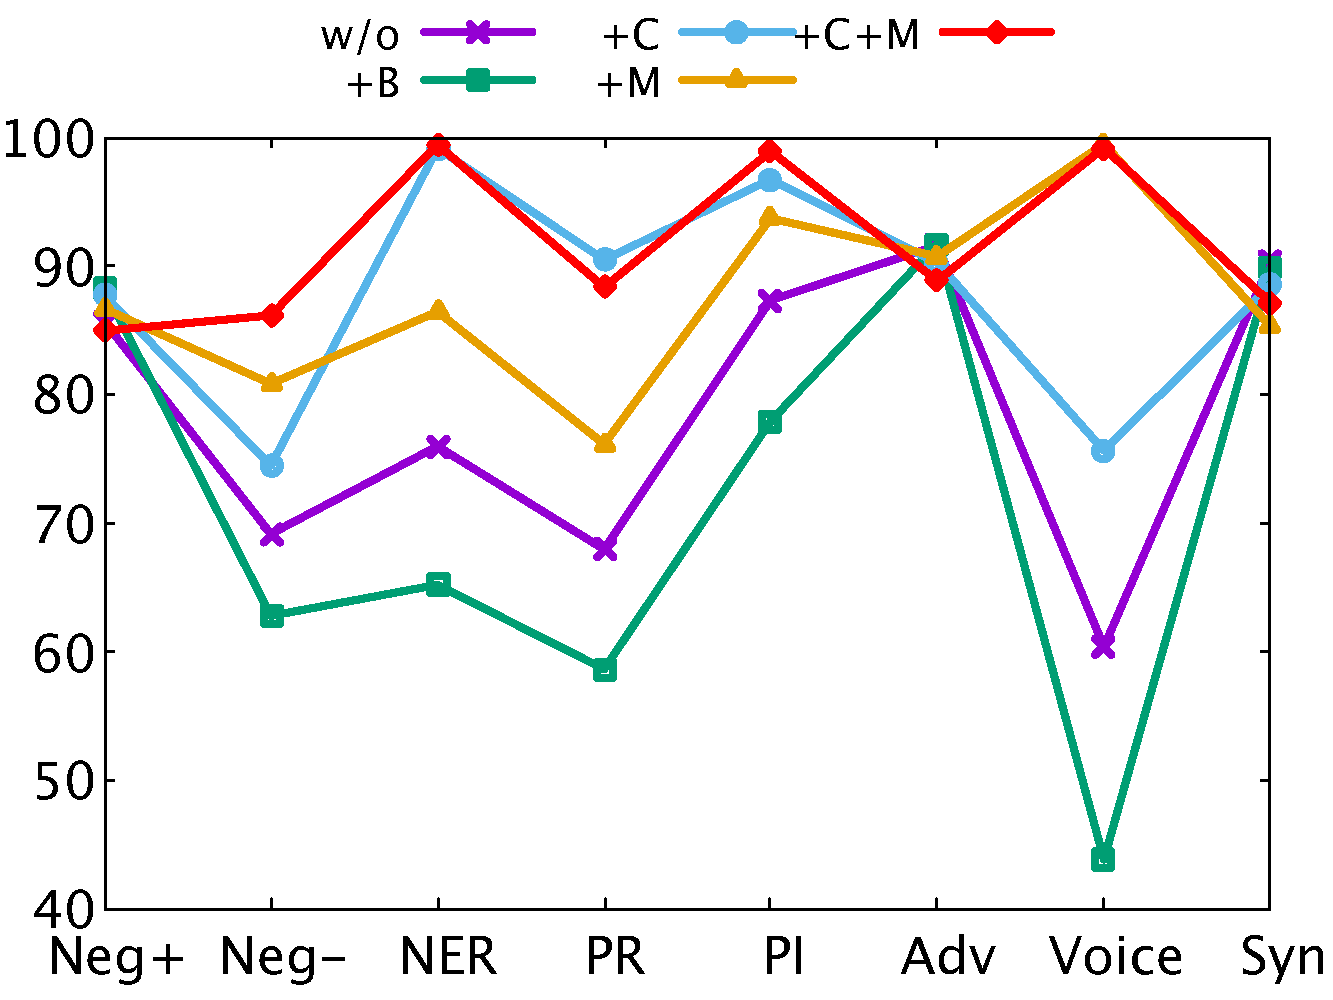
\includegraphics[width=0.6\columnwidth]{data/roc_roberta.pdf}
%   \caption{Detailed stress test with different aspects on ROC dataset. The x-axis indicates different stress test aspects and the y-axis indicates model accuracy in percentage.}
%   \label{fig:detailed}
% \end{figure}


%\begin{figure*}[!th]
%\centering
%\begin{subfigure}[b]{0.28\textwidth}
%\centering
%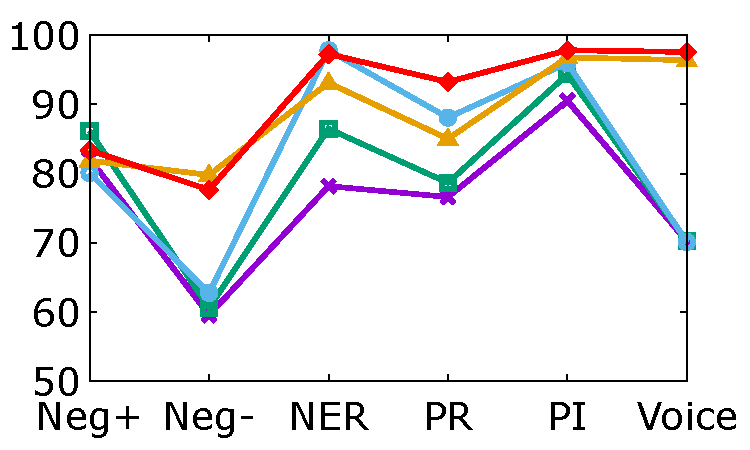
\includegraphics[width=\columnwidth]{data/roc_bert.pdf}
%\caption{BT (ROC)}
%\label{fig:roc_bert}
%\end{subfigure}
%\hfill
%\begin{subfigure}[b]{0.28\textwidth}
%\centering
%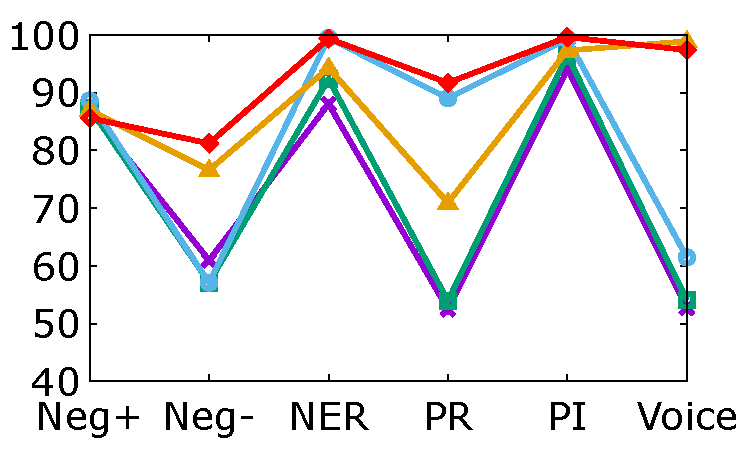
\includegraphics[width=\columnwidth]{data/roc_xlnet.pdf}
%\caption{XL (ROC)}
%\label{fig:roc_xlnet}
%\end{subfigure}
%\hfill
%\begin{subfigure}[b]{0.28\textwidth}
%\centering
%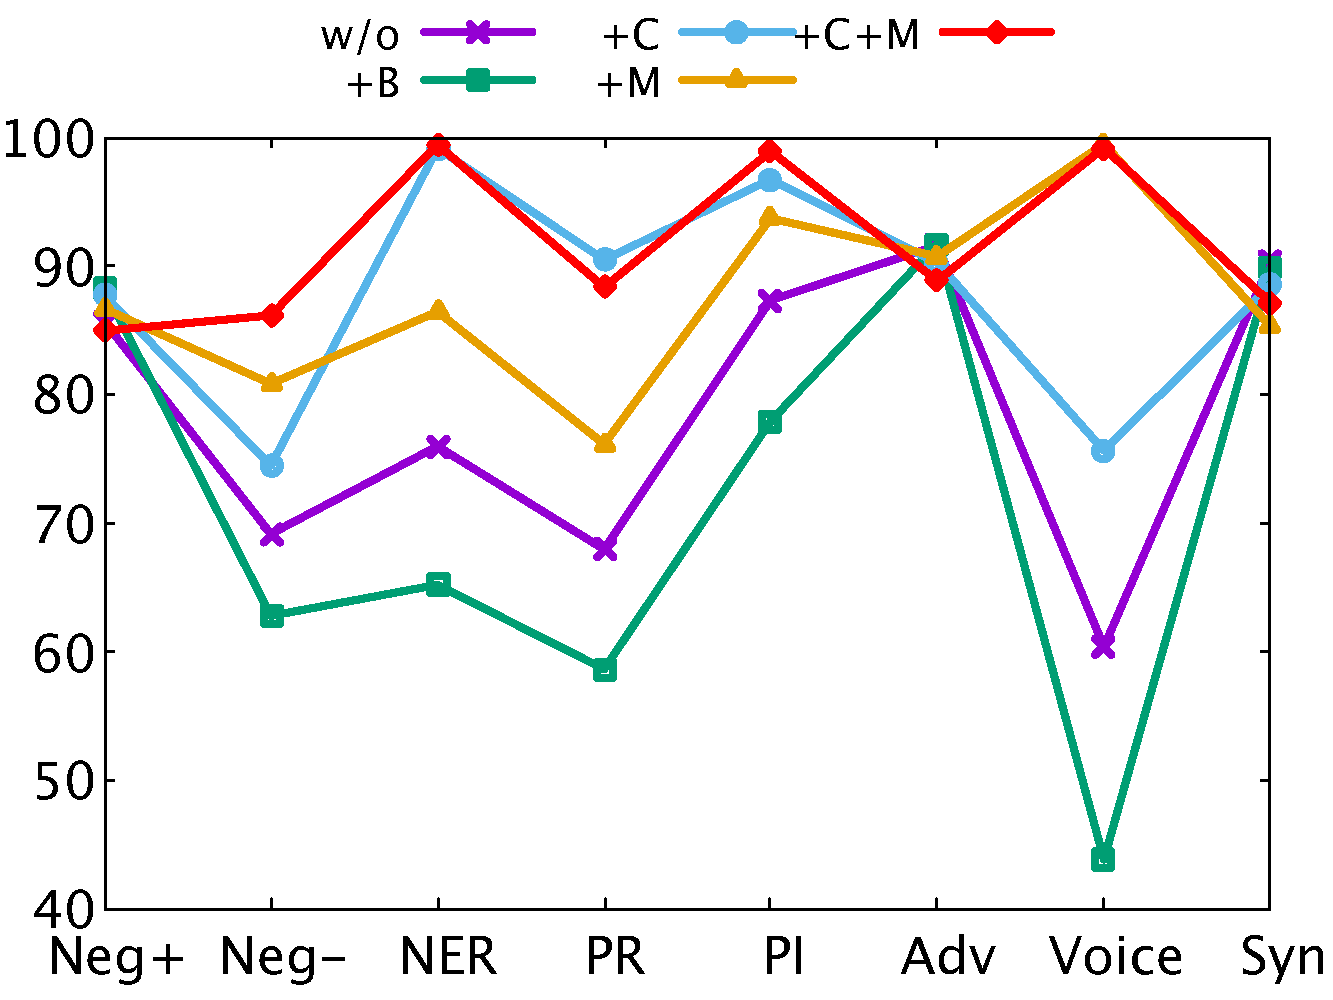
\includegraphics[width=\columnwidth]{data/roc_roberta.pdf}
%\caption{RB (ROC)}
%\label{fig:roc_roberta}
%\end{subfigure}
%\newpage
%\begin{subfigure}[b]{0.28\textwidth}
%\centering
%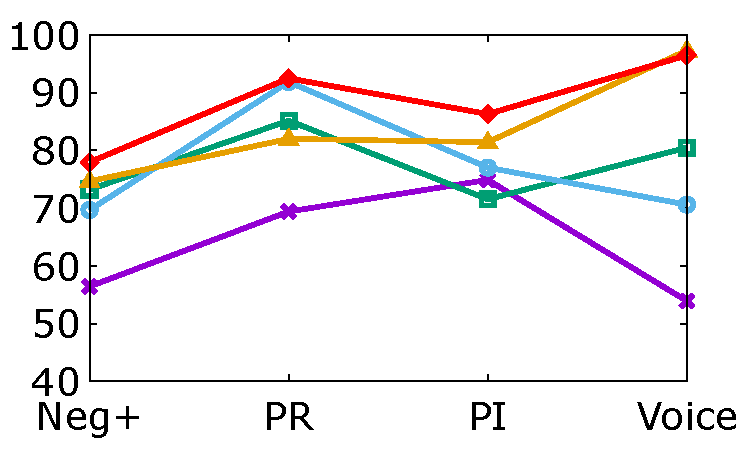
\includegraphics[width=\columnwidth]{data/copa_bert.pdf}
%\caption{BT (COPA)}
%\label{fig:copa_bert}
%\end{subfigure}
%\hfill
%\begin{subfigure}[b]{0.28\textwidth}
%\centering
%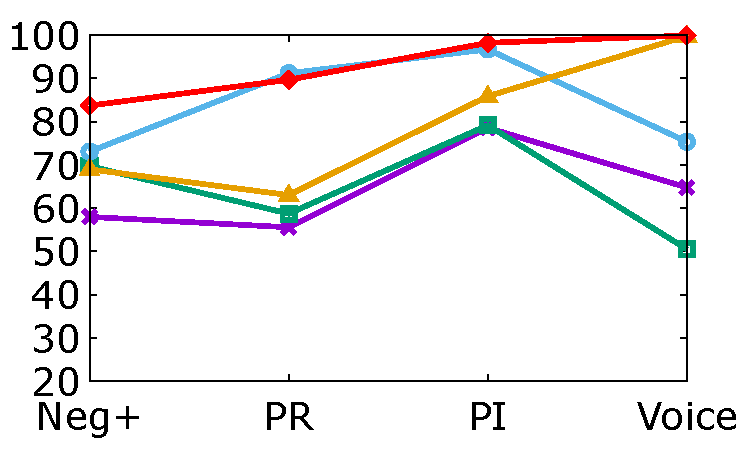
\includegraphics[width=\columnwidth]{data/copa_xlnet.pdf}
%\caption{XL (COPA)}
%\label{fig:copa_xlnet}
%\end{subfigure}
%\hfill
%\begin{subfigure}[b]{0.28\textwidth}
%\centering
%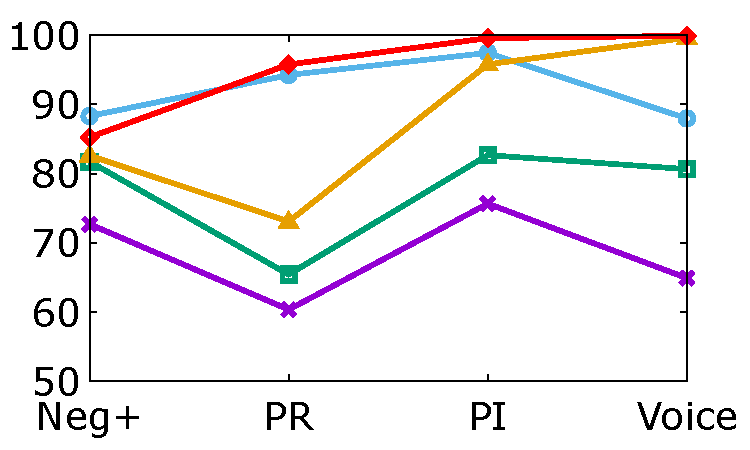
\includegraphics[width=\columnwidth]{data/copa_roberta.pdf}
%\caption{RB (COPA)}
%\label{fig:copa_roberta}
%\end{subfigure}
%\newpage
%\begin{subfigure}[b]{0.28\textwidth}
%\centering
%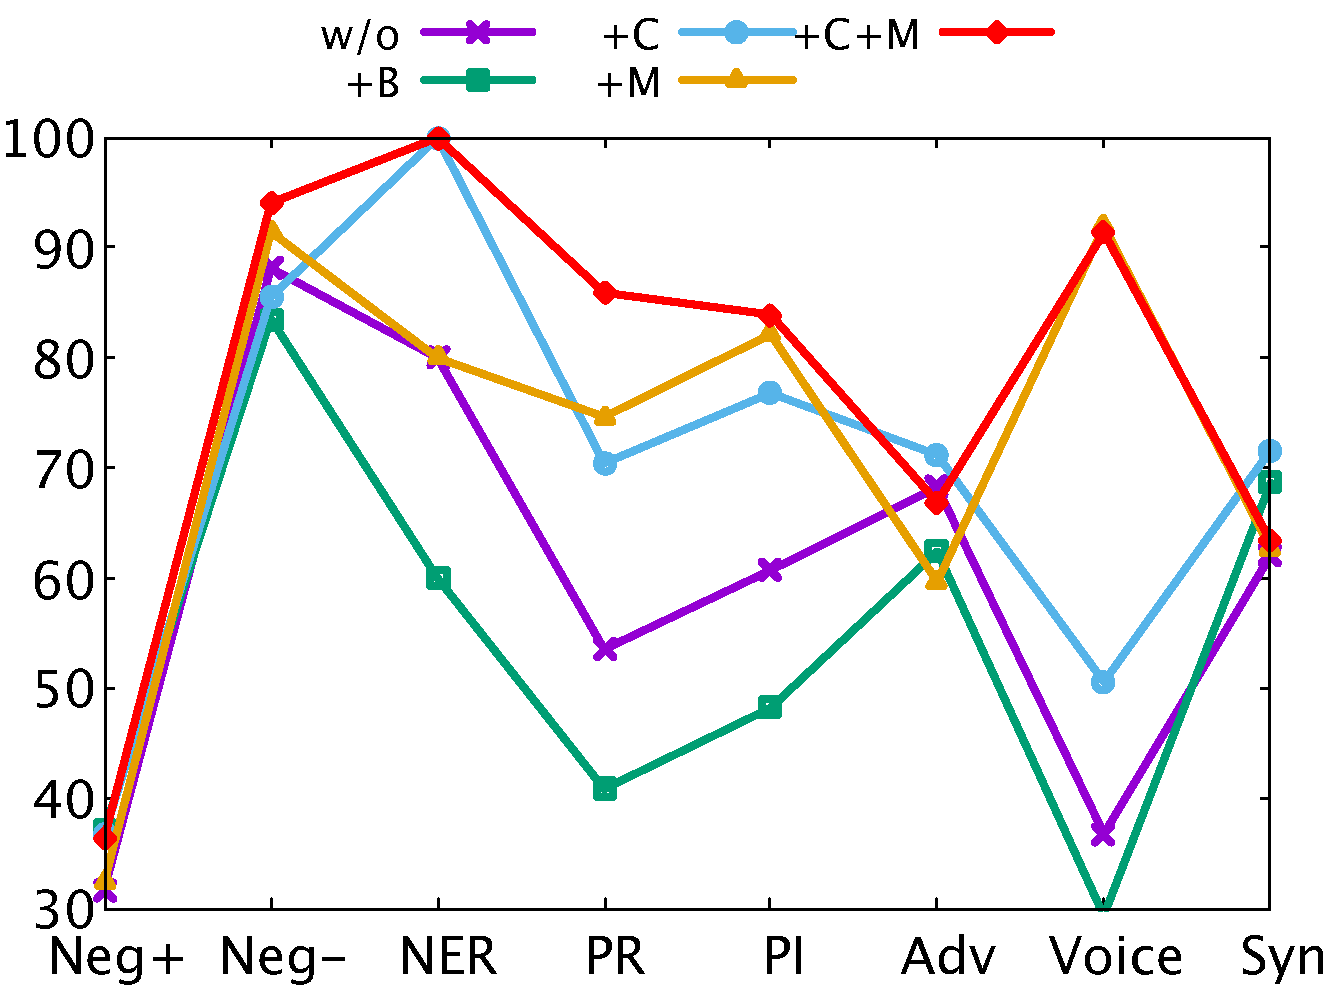
\includegraphics[width=\columnwidth]{data/arct_bert.pdf}
%\caption{BT (ARCT)}
%\label{fig:arct_bert}
%\end{subfigure}
%\hfill
%\begin{subfigure}[b]{0.28\textwidth}
%\centering
%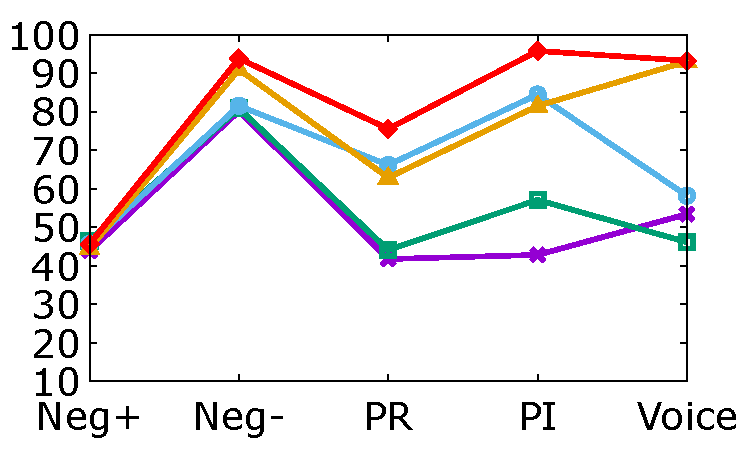
\includegraphics[width=\columnwidth]{data/arct_xlnet.pdf}
%\caption{XL (ARCT)}
%\label{fig:arct_xlnet}
%\end{subfigure}
%\hfill
%\begin{subfigure}[b]{0.28\textwidth}
%\centering
%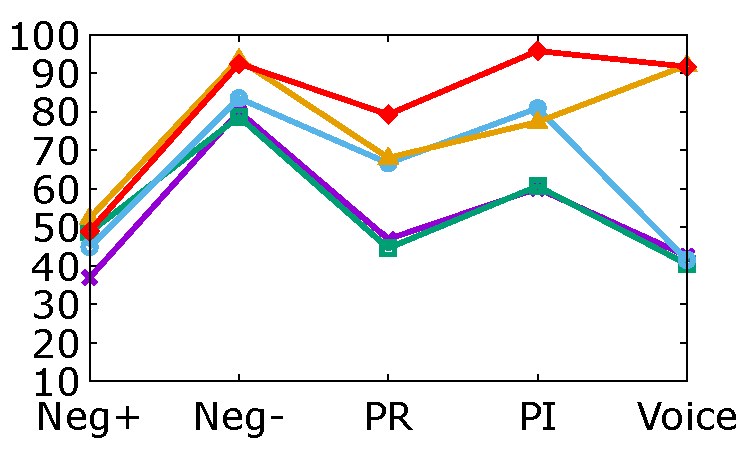
\includegraphics[width=\columnwidth]{data/arct_roberta.pdf}
%\caption{RB (ARCT)}
%\label{fig:arct_roberta}
%\end{subfigure}
%\newpage
%\begin{subfigure}[b]{0.28\textwidth}
%\centering
%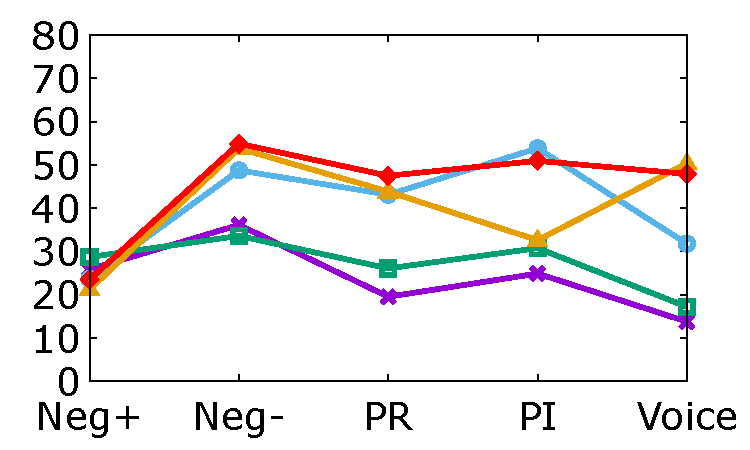
\includegraphics[width=\columnwidth]{data/reclor_bert.pdf}
%\caption{BT (RECLOR)}
%\label{fig:reclor_bert}
%\end{subfigure}
%\hfill
%\begin{subfigure}[b]{0.28\textwidth}
%\centering
%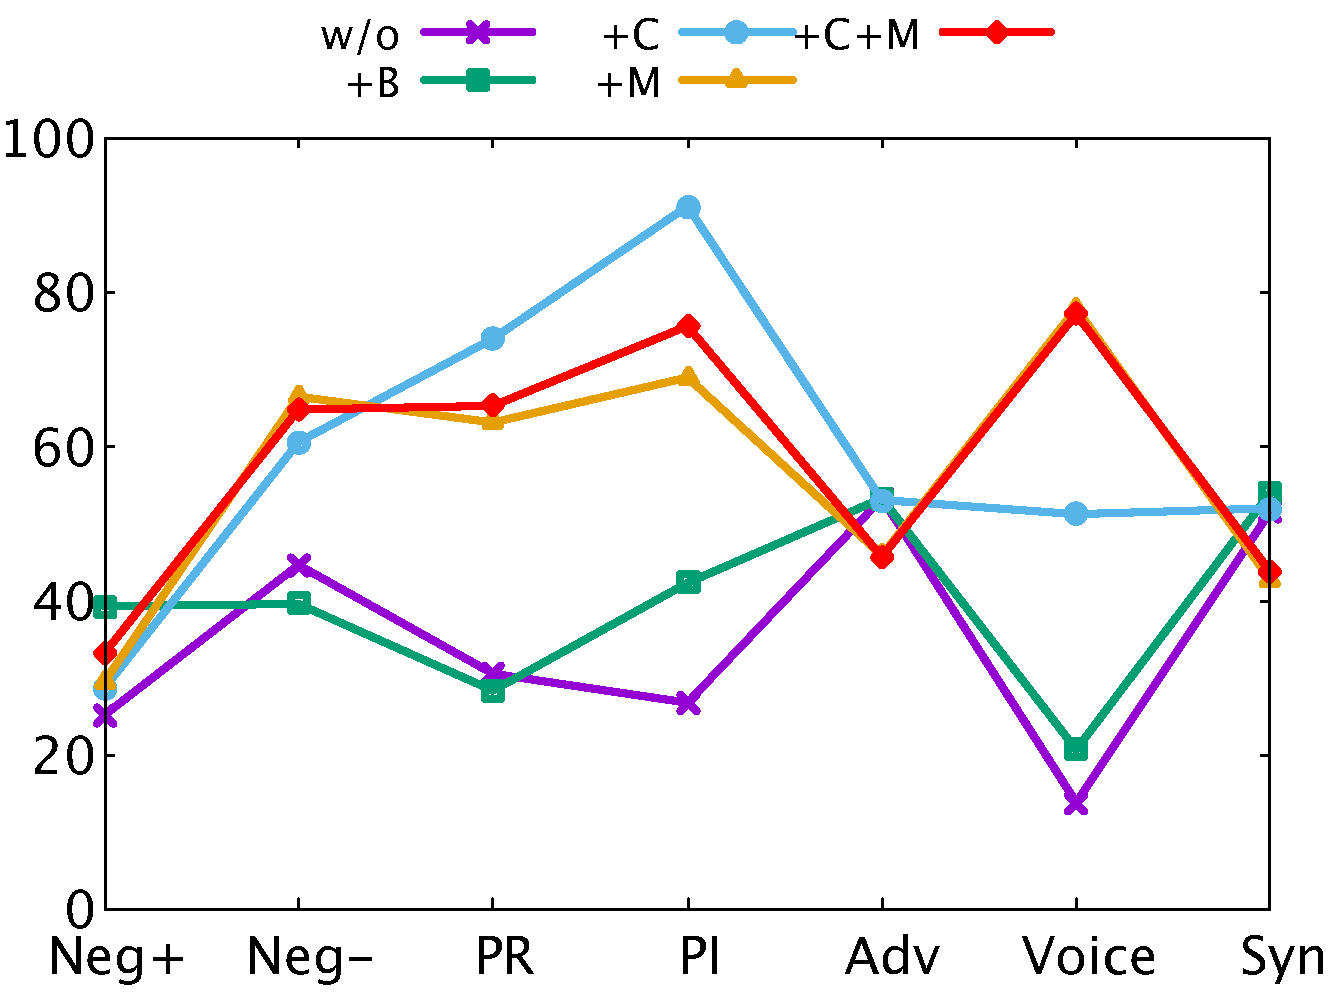
\includegraphics[width=\columnwidth]{data/reclor_xlnet.pdf}
%\caption{XL (RECLOR))}
%\label{fig:reclor_xlnet}
%\end{subfigure}
%\hfill
%\begin{subfigure}[b]{0.28\textwidth}
%\centering
%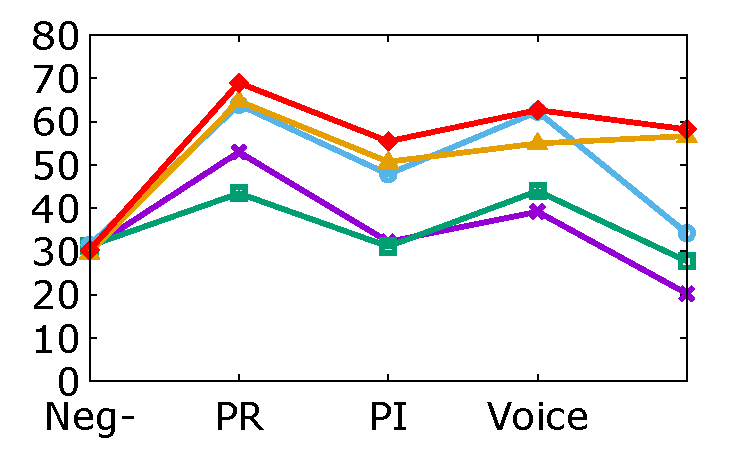
\includegraphics[width=\columnwidth]{data/reclor_roberta.pdf}
%\caption{RB (RECLOR)}
%\label{fig:arct_roberta}
%\end{subfigure}
%\newpage
%\begin{subfigure}[b]{1.0\textwidth}
%\centering
%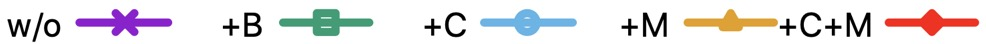
\includegraphics[width=0.4\columnwidth]{data/label.jpg}
%\label{fig:label}
%\end{subfigure}
%\caption{Fine-grained stress test with different aspects on 4 different tasks. 
%The x-axis in the figures indicates different stress test aspects and the y-axis indicates model accuracy in percentage.}
%%\KZ{Caption is wrong! most graphs are fine. 
%%But ReCLOR (RB) is a bit strange. 
%%Why is BT line exactly the same as the BT+C? And why is BT+B so bad?}}
%\label{fig:detail}
%\end{figure*}
%%
%
\begin{figure*}[!th]
\centering
\begin{subfigure}[b]{0.24\textwidth}
\centering
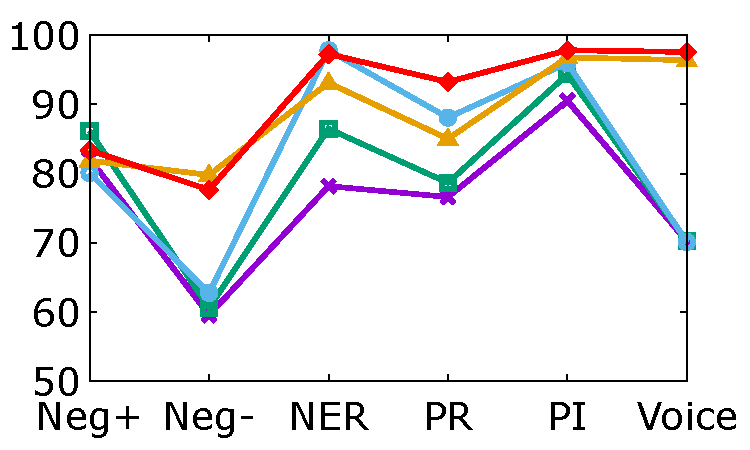
\includegraphics[width=\columnwidth]{data/roc_bert.pdf}
\caption{BT (ROC)}
\label{fig:roc_bert}
\end{subfigure}
\hfill
\begin{subfigure}[b]{0.24\textwidth}
\centering
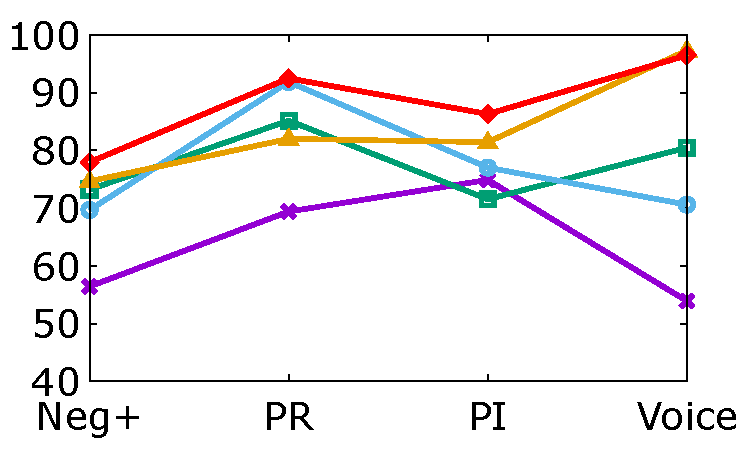
\includegraphics[width=\columnwidth]{data/copa_bert.pdf}
\caption{BT (COPA)}
\label{fig:copa_bert}
\end{subfigure}
\hfill
\begin{subfigure}[b]{0.24\textwidth}
\centering
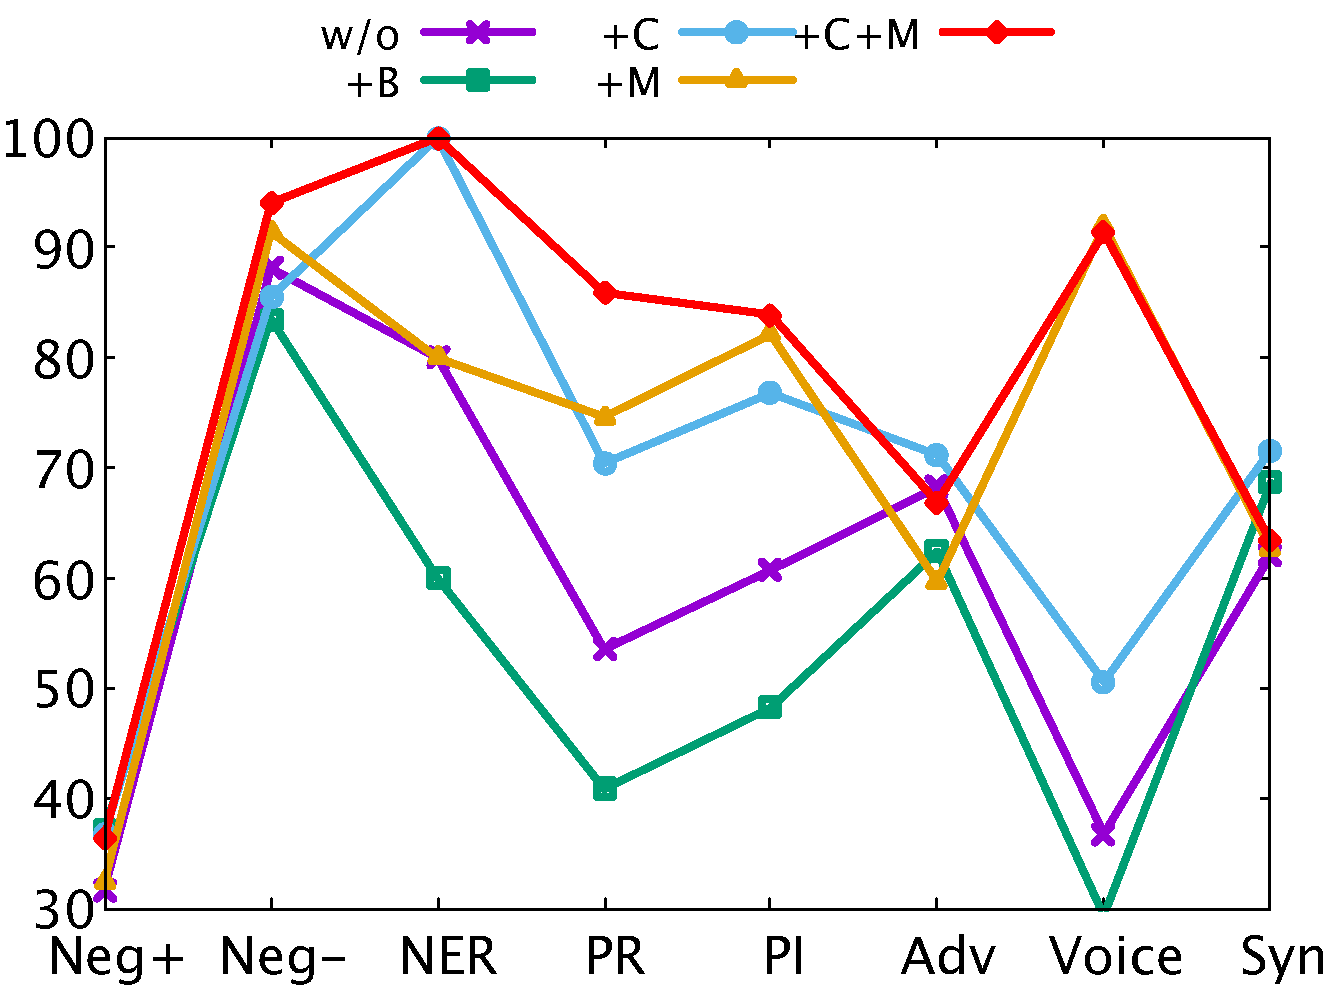
\includegraphics[width=\columnwidth]{data/arct_bert.pdf}
\caption{BT (ARCT)}
\label{fig:arct_bert}
\end{subfigure}
\hfill
\begin{subfigure}[b]{0.24\textwidth}
\centering
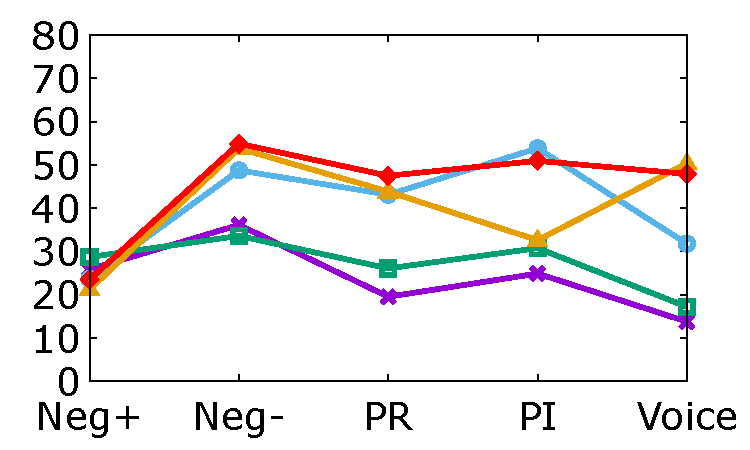
\includegraphics[width=\columnwidth]{data/reclor_bert.pdf}
\caption{BT (RECLOR)}
\label{fig:reclor_bert}
\end{subfigure}
\newpage
\begin{subfigure}[b]{0.24\textwidth}
\centering
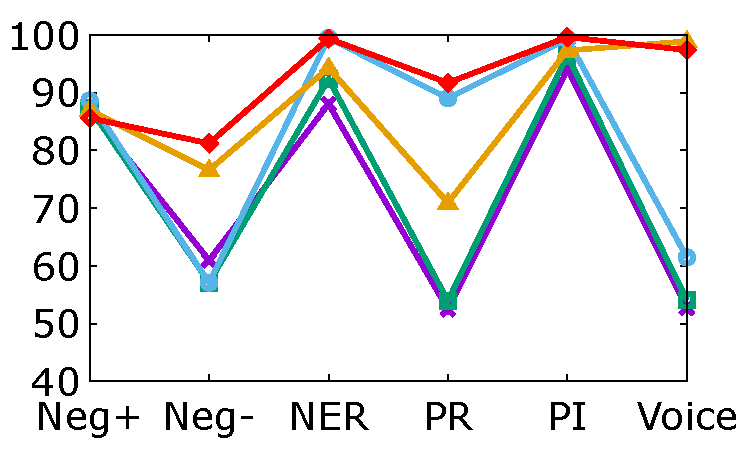
\includegraphics[width=\columnwidth]{data/roc_xlnet.pdf}
\caption{XL (ROC)}
\label{fig:roc_xlnet}
\end{subfigure}
\hfill
\begin{subfigure}[b]{0.24\textwidth}
\centering
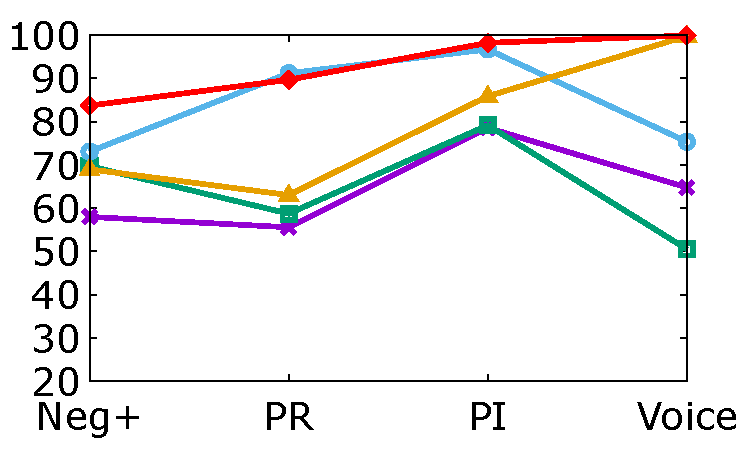
\includegraphics[width=\columnwidth]{data/copa_xlnet.pdf}
\caption{XL (COPA)}
\label{fig:copa_xlnet}
\end{subfigure}
\hfill
\begin{subfigure}[b]{0.24\textwidth}
\centering
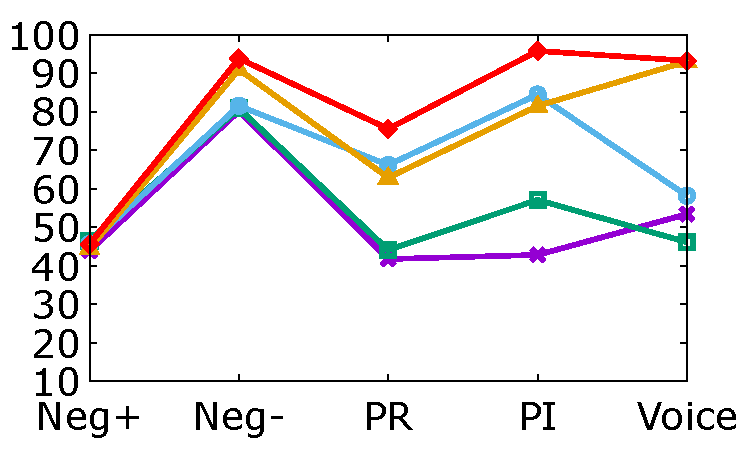
\includegraphics[width=\columnwidth]{data/arct_xlnet.pdf}
\caption{XL (ARCT)}
\label{fig:arct_xlnet}
\end{subfigure}
\hfill
\begin{subfigure}[b]{0.24\textwidth}
\centering
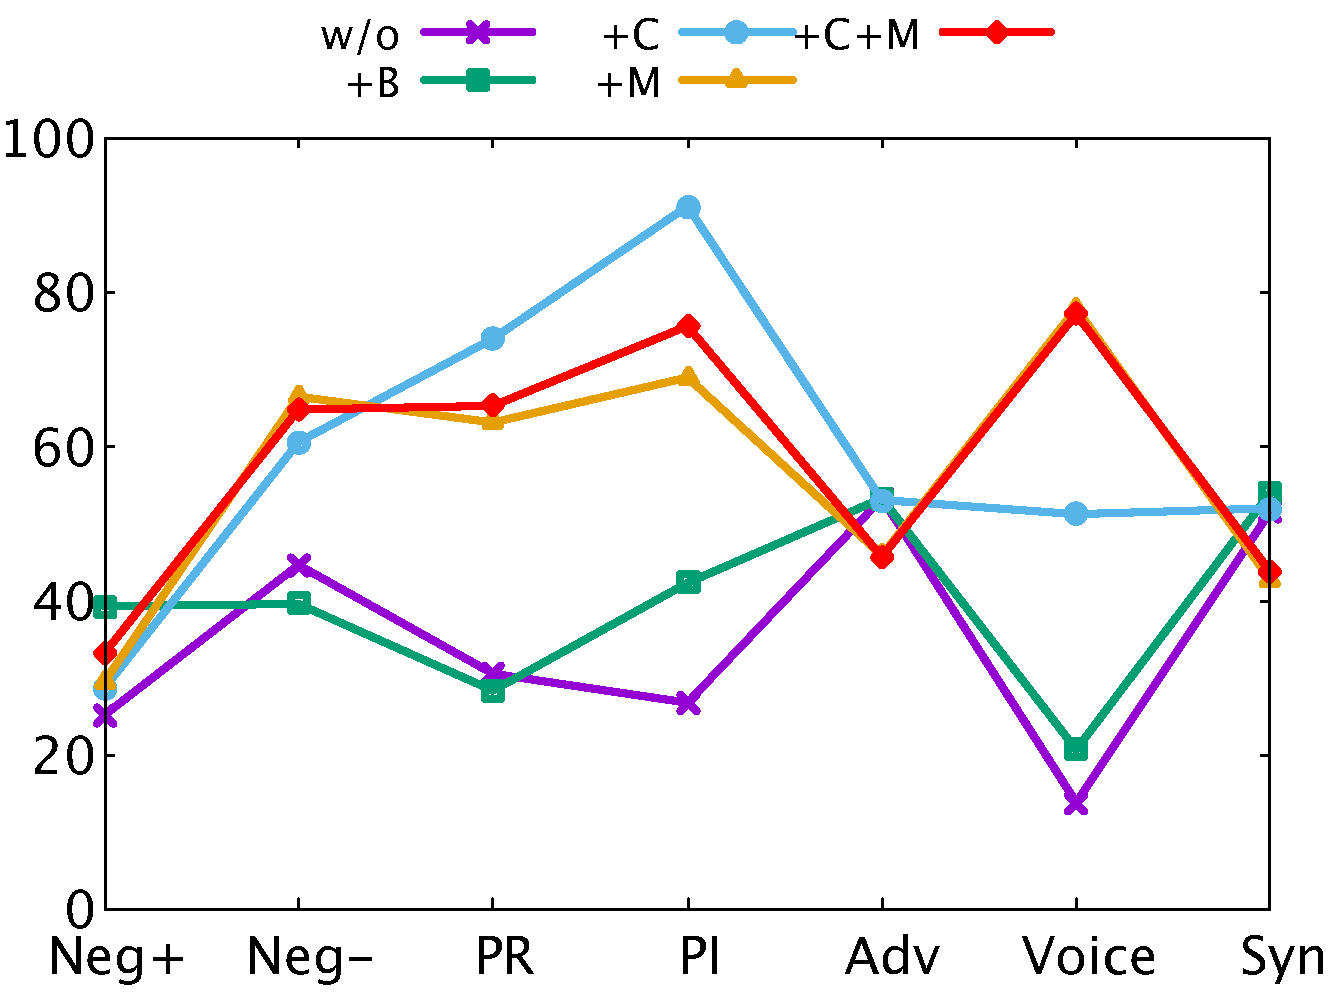
\includegraphics[width=\columnwidth]{data/reclor_xlnet.pdf}
\caption{XL (RECLOR))}
\label{fig:reclor_xlnet}
\end{subfigure}
\newpage
\begin{subfigure}[b]{0.24\textwidth}
\centering
\includegraphics[width=\columnwidth]{data/roc_roberta.pdf}
\caption{RB (ROC)}
\label{fig:roc_roberta}
\end{subfigure}
\hfill
\begin{subfigure}[b]{0.24\textwidth}
\centering
\includegraphics[width=\columnwidth]{data/copa_roberta.pdf}
\caption{RB (COPA)}
\label{fig:copa_roberta}
\end{subfigure}
\hfill
\begin{subfigure}[b]{0.24\textwidth}
\centering
\includegraphics[width=\columnwidth]{data/arct_roberta.pdf}
\caption{RB (ARCT)}
\label{fig:arct_roberta}
\end{subfigure}
\hfill
\begin{subfigure}[b]{0.24\textwidth}
\centering
\includegraphics[width=\columnwidth]{data/reclor_roberta.pdf}
\caption{RB (RECLOR)}
\label{fig:arct_roberta}
\end{subfigure}
\newpage
\begin{subfigure}[b]{1.0\textwidth}
\centering
\includegraphics[width=0.4\columnwidth]{data/label.jpg}
\label{fig:label}
\end{subfigure}
\caption{Fine-grained stress test with different aspects on 4 different tasks. 
The x-axis in the figures indicates different stress test aspects and the y-axis indicates model accuracy in percentage.}
%\KZ{Caption is wrong! most graphs are fine. 
%But ReCLOR (RB) is a bit strange. 
%Why is BT line exactly the same as the BT+C? And why is BT+B so bad?}}
\label{fig:detail}
\end{figure*}
%
\subsubsection{Fine-grained results}
\label{sec:fine-grained}
We proceed to break down the results in \tabref{tab:stressresults} into accuracies on stress tests
created by different operators. 
%We show the detailed results in~\figref{fig:detail} 
%Concretely, six different aspects of stress test data are 
%utilized for testing.
COPA and RECLOR datasets do not show all six operators
because some of the operators generate too little data
for them, as shown in \tabref{tab:cases}. 
%The x-axis in the figures indicates different stress test aspects 
%and the y-axis indicates model accuracy in percentage.
%We apply the proposed two operators \textit{crossover} and \textit{mutation} to BERT, XLNet and RoBERTa 
%models and compare it with back-translation.
%and test on various stress test cases with different aspects. 
The corresponding results are presented in~\figref{fig:detail}. 
We observe that the vanilla model in purple and back-translation in green show
worse results across different aspects than other lines. 
The models trained with data augmented by \textit{crossover} and \textit{mutation} 
(the red lines) are generally more robust than others.
%\KZ{It is consistent with our overall results in~\tabref{tab:results}.} 
Please refer to Appendix A. 
%\footnote{There are some dashes in the table because the } 
for complete results. 
%\KZ{You need to explain why there are some dashes in the table in appendix.}

%We also observe that the 
%accuracy performance points for ``Syn'' and ``Adv'' are concentrated 
%but scattered on other operator aspects. 
Since every type of stress tests 
%(except ``Syn'' and ``Adv) 
can evaluate if a model is robust, particularly if it considers the 
premise by giving it two very similar choices, 
the above results on the stress tests of all types show that our two methods do 
%improves the model robustness, and may even encourage the models to look toward the
reduce short-circuits, and may even encourage the models to look toward the
premises.
We will provide additional pieces of evidence to confirm this in the next two subsections.

%\KZ{The weakness can be on the same table as the improvements
%to save space.}
%\KZ{Check the following analysis to make sure it's consistent with the tables.}

%Compared with 
%base models without data augmentation, we find that 
%all four data augmentation methods moderately improve
%the models when tested on the original test set. 
%In ROC, accuracy of BERT and RoBERTa trained with crossover augmented data 
%exceeds base models and ranks top. Crossover method also works on COPA. 
%Even though back-translation obtains higher score mostly on ARCT and RECLOR,
%crossover, mutation and crossover+mutation barely fall below the base model. 
%
%Augmentation fares much better in the ``Stress'' columns, though
%different methods show varying degree of success.
%Compared with the model without data augmentation, 
%the performance of models with crossover 
%has always been greatly improved (i.e., by 21.44\% for BERT on COPA).
%It indicates that reducing the short circuits 
%is a good way to improve the robustness of a model.
%The performance of new models with crossover has 
%great improvement for all models on different dataset 
%compared with the model without data augmentation, like 21.44% for BERT on COPA. 
%Mutation alone can also help with robustness on stress test better than crossover.
%This result suggests that mutation is a good method 
%for enhancing the robustness of models. 
%Though, mutation may be not a 
%good method to decrease the short circuits (\secref{sec:fix-sc}). 
%Overall, crossover+mutation 
%can mostly get the best performance on the stress test except for 
%training on RECLOR with RoBERTa. 
%to This result indicates that this kind of data can prevent models from being confused 
%by simple perturbations thus improving the robustness of models. 
%Besides, we can also find that back-translation doesn't improve the models' robustness much.
%Crossover alone can also help with robustness on stress test but 
%no better than mutation and crossover+mutation.  

%some of Table 5's AW scores being 
%some of Table 5's AW scores being 
%lower than AW for model w/o augmentation (e.g., 45.13 in (b)), 
%then the reason is AW is only a proxy test
%that catches majority of short circuit cases in our opinion, 
%but it's not perfect, as we pointed out in A2 of R1. 
%If you are referring to some accuracies in the Original columns 
%being lower than models w/o augmentation in Table 5 (e.g., 72.6 in (b)), 
%the reason is some models w/o augmentation might have 
%"cheated" to get high accuracy. Augmenting (C or M) corrects the
%biases in these models and may reduce the accuracy on the original test set.
%Nevertheless, all models after augmentation do better on the stress tests.

%have least short circuits based on BERT and XLNet. 
%Crossover+mutation based on RoBERTa takes less short circuits than others. 
%In the CO and AW columns, the result are consistent on ROC. 

%\subsection{White-box Attention Weights~(AW)}
%\KZ{Here we first talk about human testing by visualizastion,
%then talk about how to automatic it thru code.}

%show human annotation results of bert, roberta, xlnet.
%For exploiting whether attention-based models are suffered from short circuits, 
%we propose to 
%use the AW method which we have described in~\secref{}.
%It is noted that t\_1 is greater than t\_2. 
%Here t\_1 and t\_2 are tuned to 0.14 and 0.13 separately.

\subsection{Choice-only Test}
\label{sec:choice-only}

%In this section, we use choice-only test for different models on four tasks. 
%We have shown the effectiveness of \textit{crossover} and \textit{mutation} on in robustness test. 
The end-to-end test has shown the success of our data augmentation 
methods. To further explore the reason behind the performance gain, 
we also use choice-only test here.

%somewhat confirm the reason for model improvement with data augmentation 
%strategies. Moreover, this test is used to further explore 
%whether our strategies can encourage models pay more attention to premise.
In choice-only test, we only feed choices into a model without a premise which is replaced 
by an empty string. This way, 
models cannot utilize the relationship between premise and choices. 
%what we can know whether a model can 
%solve cases easily without awaring premise by test accuracy. 
Normally, we would expect the model to make arbitrary choices.
However, if a model can easily ``guess'' the ``right'' choice which 
normally requires the relationship between premise and choices,  
one possibility is that this model cheats on evaluation procedure and 
may be fragile. Thus, the higher score may indicate more use of short-circuits.

In~\figref{fig:choice-only}, we observe that in choice-only tests,
the accuracy of models augmented with \textit{crossover} and \textit{mutation} 
(red line) drops the most. 
Sometimes the performances are similar to random selection, e.g., 
RB+C+M on ARCT (56.38\%), which indicates that models 
are no longer cheating. 
In other words, models augmented by crossover and mutation 
are more likely to consider the premises. 
The results on the choice-only tests provide another perspective for us
to re-assure that models augmented with crossover and mutation can reduce
short circuits and thus model fragility.

%\KZ{Rephrase: 
%However, another possibility reason for lower choice-only test accuracy 
%that is also not ruled out is that 
%even if the model can tell the result with only choices, 
%it still chooses to look at the premise context. 
%Although high scores do not necessarily imply models 
%are not looking forward, low scores necessarily mean that models cannot 
%conclude that solely relying on choices.} 

%\begin{table}[th]
%\centering
%\scriptsize
%\begin{tabular}{c|rrrr}
%\toprule
%\textbf{Model} & \textbf{ROC} & \textbf{COPA} & \textbf{ARCT} & \textbf{RECLOR} \\ \midrule
%%BT  &98.76 &89.68&\textbf{99.65}&82.46    \\ \hline
%%BT+B  &99.26 &96.79   &99.34  &86.01  \\ \hline
%%BT+C  &\textbf{99.69} &\textbf{98.35}&98.37   &80 \\ \hline
%%BT+M  &99.26 & 95.17 &98.67 &82.48    \\ \hline
%%BT+C+M  &98.82 &96.96 &98.00 &\textbf{96.79}  \\ \midrule
%%XL  &28.08 &93.16 & 85.67 & 79.64 \\ \hline
%%XL+B  &19.27  &91.46 &95.73 & 81.40   \\ \hline
%%XL+C  &\textbf{64.58} &45.13  &55.59  &\textbf{87.87} \\ \hline
%%XL+M  &62.77  &96.85 & \textbf{95.74}& 72.76  \\ \hline
%%XL+C+M  &60.25 & \textbf{98.51}&86.26 &   48.71\\ \midrule
%%RB  &77.41 & 80.89 & 99.14& 85.88 \\ \hline
%%RB+B  &   58.15 &\textbf{96.36}   & 97.78& 15.69  \\ \hline
%%RB+C  &   82.71& 89.62&79.19& 89.68\\ \hline
%%RB+M  &71.73& 62.26& \textbf{100.00}&\textbf{100.00}  \\ \hline
%%RB+C+M  &\textbf{93.31} &61.89    &71.47 & 89.26\\ 
%%
%BT (w/o)&54.62&51.4&61.94&42.8 \\ \hline
%BT+B&58.26&50.8&64.41&39.2  \\ \hline
%BT+C&51.2&48.2&55.63&30.8  \\ \hline
%BT+M&51.79&48.8&55.18&38   \\ \hline
%BT+C+M&43.56&49.4&52.03&33.8  \\ \midrule
%XL (w/o)&71.14&57&65.99&42.2 \\ \hline
%XL+B&73.17&60&66.89&41.4  \\ \hline
%XL+C&65.63&55&55.86&34.2  \\ \hline
%XL+M&71.94&57.8&66.22&42  \\ \hline
%XL+C+M&66.22&58.4&62.84&35  \\ \midrule
%RB (w/o)&73.97&59.4&67.79&30.2 \\ \hline
%RB+B&74.77&61.4&69.37&42.2  \\ \hline
%RB+C&73.06&58.4&68.47&34.6  \\ \hline
%RB+M&70.34&56&61.49&40      \\ \hline
%RB+C+M&71.3&54.8&67.79&32.2  \\ 
%\bottomrule
%\end{tabular}
%\caption{Choice-only test for transformer-based models on 4 datasets. All numbers are percentages (\%)}
%%\KZ{I assume this is the ending-only test? But isn't scriptsizeer the better
%%for ending-only tests?}}
%\label{tab:only-test}
%\end{table}
%
\begin{figure}[th]
    \centering
    \includegraphics[width=0.7\columnwidth]{data/choice-only.pdf}
    \caption{Choice-only test: Accuracies of different data augmentation methods with 3 models on 4 tasks. 
    The detailed numbers are in Appendix B.}
    \label{fig:choice-only}
\end{figure}

However, one may argue that even if a model can 
choose or ``guess'' correctly given only the choices but no premise, 
it may still have the ability to look at the premise if it's given one,
like in the end-to-end test.
Therefore, next we conduct an additional case study to show that short-circuit
does take place and our augmentation methods alleviate it.

\subsection{Case Study}
\label{sec:case}

%\begin{figure}[th!]
%\centering
%\begin{subfigure}[b]{0.21\textwidth}
%\centering
%
%\framebox{\includegraphics[width=\columnwidth]{figure/case_original.eps}}
%\caption{RB(w/o)}
%\label{fig:case_original}
%\end{subfigure}
%\hfill
%\begin{subfigure}[b]{0.21\textwidth}
%\centering
%\framebox{\includegraphics[width=\columnwidth]{figure/case_b.eps}}
%\caption{RB+B}
%\label{fig:case_b}
%\end{subfigure}
%\hfill
%\newpage
%\begin{subfigure}[b]{0.21\textwidth}
%\centering
%\framebox{\includegraphics[width=\columnwidth]{figure/case_c.eps}}
%\caption{RB+C}
%\label{fig:case_c}
%\end{subfigure}
%\hfill
%\begin{subfigure}[b]{0.21\textwidth}
%\centering
%\framebox{\includegraphics[width=\columnwidth]{figure/case_cm.eps}}
%\caption{RB+C+M}
%\label{fig:case_cm}
%\end{subfigure}
%\caption{Attention map on a COPA example for models.}
%%\KZ{Caption is wrong! most graphs are fine. 
%%But ReCLOR (RB) is a bit strange. 
%%Why is BT line exactly the same as the BT+C? And why is BT+B so bad?}}
%\label{fig:case}
%\end{figure}
%

%In \figref{fig:case}, 
%%illustration. There is no positive attention value in front of the 
%%fourth sentence, so we intercept it from where it is worth. 
%RoBERTa trained on the original training set fails to pick up the 
%relation between ``pushed'' and ``opened''. 
%%right choice likely due to there being virtually no attention 
%%connection between words in the choice and words in the premise. 
%After training with \textit{crossover} data augmentation, 
%the model learns to build contextual reasoning  
%by attending to relevant concepts in the premise. 
%%i.e., ``show'' in this example. The rationale behind 
%%such a change of attention pattern is that, 
%%in a MCQ created by crossover operation, 
%%the model needs to combine information 
%%in the premise to effectively 
%%distinguish the true ``right'' choice from the wrong one, 
%%which is also a right choice in another MCQ. 
%to have not enhanced such abilities. We provide additional cases in Appendix C.

%\begin{figure}[th]
%\centering
%{\setlength{\fboxsep}{0pt}
%5\framebox{%
%\includegraphics[width=0.47\columnwidth]{figure/o_un.eps}
%}
%\hfill
%\framebox{%
%\includegraphics[width=0.47\columnwidth]{figure/cross_un.eps}
%}
%}
%\caption{Attention maps showing that RoBERTa short-circuits on a ROC
%question (left) and no longer short-circuits after data augmentation (right). \KZ{I suggest we show a few more cases here to be more convincing. Show the before and after. Before there's no attention to the
%premise, after there is.}}
%\label{fig:case_study}
%\end{figure}

%\begin{example}\label{ex:roc}
%An MCQ from ROC:\\ \\
%\noindent
%\textbf{Premise:} Sarah was home alone. She wanted to stay busy. She turned on the TV. 
%She found a reality show to watch.  \\
%\textbf{Choice 1:} Sarah then happily watched the show.  \checksymbol  \\
%\textbf{Choice 2:} Sarah could not find anything to watch. \crosssymbol
%\end{example}

Our case study is a series of white-box tests that demonstrate
the change in attention patterns.

We take an example from ROC which is shown in~\tabref{table:dataset}.
We explore BERT-based models by 
analyzing their attention maps on this case in~\figref{fig:roc_bert}.  
In this example, the word ``show'' in the premise is strongly
related to the token ``reality show'' in the right choice from human knowledge. 
%The relationship between these two words is the key to answering this question. 
%We explore different models with the augmentation method with attention map 
%to visualize if these two words have a relationship or not.
The attention map is visualized via an off-the-shelf tool~\cite{vig-2019-multiscale}.


There is no positive attention value in front of the fourth sentence, 
so we intercept it from where it is worth. 
BERT trained on the original training set fails 
to pick up the right choice likely due to there being 
virtually no attention connection between words in 
the choice and words in the premise.
After training with \textit{crossover} data augmentation, 
the model learns  
to pay attention to the premise and the relationship 
between premise and choices. 
i.e., ``show'' in this example. 
Similar trends also exist for the \textit{mutation} operation in \figref{fig:roc_m} 
and the combination of \textit{crossover} 
and \textit{mutation} operation in~\figref{fig:roc_cm}. 
The rationale behind 
such a change of attention pattern is that, 
in an MCQ created by \textit{crossover} operation (\figref{fig:roc_c}), \textit{mutation}(\figref{fig:roc_m}), 
and the combination of them (\figref{fig:roc_cm}), 
the model needs to combine the information 
in the premise to effectively 
distinguish the true ``right'' choice from the wrong one. 
However, the light and sparse attention color blocks on the attention map for back-translation 
in \figref{fig:roc_b} indicate back-translation 
can not help BERT connect the choice and premise very well in this question.
These observations empirically demonstrate the effectiveness of our methods 
in encouraging the model to pay attention to the premise to reduce 
short circuits. We provide additional cases in Appendix C. 

%\begin{figure}[th!]
%\centering
%\begin{subfigure}[b]{0.35\textwidth}
%\centering
%\framebox{\includegraphics[width=\columnwidth]{figure/roc_b.eps}}
%\caption{BT+B}
%\label{fig:roc_b}
%\end{subfigure}
%\hfill
%\begin{subfigure}[b]{0.35\textwidth}
%\centering
%\framebox{\includegraphics[width=\columnwidth]{figure/roc_c.eps}}
%\caption{BT+C}
%\label{fig:roc_c}
%\end{subfigure}
%%\hfill
%\newpage
%\begin{subfigure}[b]{0.35\textwidth}
%\centering
%\framebox{\includegraphics[width=\columnwidth]{figure/roc_m.eps}}
%\caption{BT+M}
%\label{fig:roc_m}
%\end{subfigure}
%\hfill
%\begin{subfigure}[b]{0.35\textwidth}
%\centering
%\framebox{\includegraphics[width=\columnwidth]{figure/roc_cm.eps}}
%\caption{BT+C+M}
%\label{fig:roc_cm}
%\end{subfigure}
%\caption{Attention map on a ROC example for BERT-based models.}
%%\KZ{Caption is wrong! most graphs are fine. 
%%But ReCLOR (RB) is a bit strange. 
%%Why is BT line exactly the same as the BT+C? And why is BT+B so bad?}}
%\label{fig:roc_bert}
%\end{figure}
%
\begin{figure}[h!]
\centering
\begin{minipage}{0.30\linewidth}
    \centering
    \fbox{\includegraphics[width=\linewidth]{figure/roc_b.eps}}
    \caption*{BT+B}
    \label{fig:roc_b}
\end{minipage}
\hspace{0.5cm}
\begin{minipage}{0.30\linewidth}
    \centering
    \fbox{\includegraphics[width=\linewidth]{figure/roc_c.eps}}
    \caption*{BT+C}
    \label{fig:roc_c}
\end{minipage}
\hspace{1.5cm}
\vspace{0.5cm}
\begin{minipage}{0.30\linewidth}
    \centering
    \fbox{\includegraphics[width=\linewidth]{figure/roc_m.eps}}
    \caption*{BT+M}
    \label{fig:roc_m}
\end{minipage}
\hspace{0.5cm}
\begin{minipage}{0.30\linewidth}
    \centering
    \fbox{\includegraphics[width=\linewidth]{figure/roc_cm.eps}}
    \caption*{BT+C+M}
    \label{fig:roc_cm}
\end{minipage}
\caption{Attention map on a ROC example for BERT-based models.}
\label{fig:roc_bert}
\end{figure}


%\subsection{Discussion}
%
%From previous test results on original test, stress test, choice-only test and test cases analysis, 
%we can illustrate that \textit{crossover} and \textit{mutation} can teach models to pay more attention to 
%the relationship between the premise and the choices. However, there is a doubt that \textit{mutation} 
%can triger a new bias cue that once the model find the choice is ingrammatically, it will choose another 
%choice. 
%%Thus we make another experiment to verify whether the augmentation operator \textit{mutation} can 
%Thus in this section, we make an experiment that we generate new grammar test cases which only 
%mutate words in the right choices. If models' prediction results are unchanged, 
%it can indicate that these models which trained with augmentation 
%data can't be easily triggered by the grammatical cues. The test result for models are shown in \tabref{tab:mutate} on ROC dataset. 
%We can find that the predicting change rate for +M models are not higher than vanilla models which illustrates 
%that +M will not introduce extra grammatical bias cues.
%\begin{table}[th!]
%   \centering
%   \scriptsize
%   \begin{tabular}{lc}
%       \toprule
%       \textbf{Model}& Change Rate \\
%       \midrule
%       BT(w/o)& 7.35\\
%       BT+M&6.37\\
%       \midrule
%       XL(w/o)&8.17 \\
%       XL+M&8.45 \\
%       \midrule
%       RB(w/o)&5.94\\
%       RB+M&5.73\\
%       \bottomrule
%   \end{tabular}
%   \caption{Grammatical sensitivity test on ROC dataset. All the numbers are percentage(\%)}
%   \label{tab:mutate}
%\end{table}



\section{Related Work}
\paragraph{Clarification Question Generation} The concept of CQ can be naturally raised in a dialogue system where the speech recognition results tend to be erroneous so that we raise CQs for sanity check \citep{stoyanchev2014towards}, or the intents for a task is incomplete or ambiguous in a first short utterance and further CQs are needed to fill in the slots \citep{dhole2020resolving}. The concept is then extended to IR to clarify ambiguous queries \citep{aliannejadi2019asking}, and has been successfully put into practice \citep{zamani2020generating}. Other application areas including KBQA \citep{xu2019asking} and open-domain dialogue systems \citep{aliannejadi2020convai3}. CQGen can also be applied to help refine posts on websites like StackExchange \citep{Kumar_2020} and Amazon \citep{rao2019answer}. In this context, our work closely follows the research line of \citep{rao2018learning, rao2019answer, cao2019controlling}. \citet{rao2018learning} first adopted a retrieval-then-rank approach. They \citep{rao2019answer} then proposed a generation approach to train the model to maximize the utility of the hypothetical answer for the questions with GAN, to better promote specificity. \citet{cao2019controlling} propose to control the specificity by training on data with explicit indicator of specificity, but it requires additional specificity annotation. Towards the similar specificity goal, we adopted a different keyword-based approach. They also assume generating one question per context, which we claim is not sufficient to cover various possible information needs, and thus propose the task of the diverse CQGen.

\paragraph{Diverse Generation} The demand for diverse generation exists in many other fields~\cite{vijayakumar2018diverse, LiangZ18code, shen2019mixture}, and we've drawn inspirations from these literatures. For image captioning, we may use multiple descriptions for different focusing points of a scene. \textit{Diverse Beam Search} \citep{vijayakumar2018diverse} was proposed to broaden the searching space to catch such diversity by dividing groups in decoding and imposing repetition penalty between them. For machine translation, a context can be translated with different styles. \citet{shen2019mixture} thus proposed \textit{Mixture of Expert} models including hMup to reflect various styles with a discrete latent variable (\textit{expert}). And here for CQGen, diversity is required to cover various potentially missing aspects, so we come up with the idea to use keywords as a controlling variable like \textit{expert} to promote diversity.


%\section{Future Work}
%%To this end, we have successfully built a system
%%which can solve the top-$k$ extraction problem
%%with adequate accuracy and efficiency.
%%With the big data experiment result,
%%we have built a top-$k$ database with
%%over 1.7 million top-$k$ lists of 92.0\% precision.
%%In the future, we will mainly focus on three aspects of work.
%
%The first One is to further enrich the top-$k$ database
%and improve its quality. On the one hand,
%we can use larger training data and
%more sophisticated machine learning models to
%upgrade the system performance;
%on the other hand, we can explore the other source
%of top-$k$ lists rather than top-$k$ pages.
%The slide-show pages can be a good candidate (e.g. Fig. \ref{fig:slideshow}),
%as the top-$k$ list spans across a set of pages, which are connected one another
%by hyperlinks. Intuitively, we can develop a crawler that goes through
%``Previous'' and ``Next'' links and obtain a slide-show page chain.
%But the main challenge is we can not run it on big data as the web snapshot
%cannot support random access (access by URL).
%Furthermore, the snapshot may lose some nodes in a page chain,
%thus we cannot extract the complete list.
%
%The second is to further understand top-$k$ lists, especially the top-$k$ titles.
%In Section \ref{sec:problem}, we define a function $tr$ to convert a textual title
%into a five-tuple representation, which is implemented by Title Classifier.
%However, this representation remains rough as we miss some modifiers other than time and location.
%For example, ``top 10 NBA players alive'' is different from ``top 10 NBA players who have a ring'',
%but they will share the same representation. We may need to include those modifiers in the representation,
%and redefine $tr$ as $tr : (t, d) \rightarrow \mathcal{R} = (k, c, \alpha,
%\mathcal{M})$ where $\mathcal{M}$ is a set of modifiers including the temporal modifier $\tau$ and
%spatial modifier $\sigma$. To do this, we need to improve our Title Classifier to recognize general modifiers,
%probably using the same technology.
%A harder challenge is to calculate semantical similarity between $\mathcal{R}$.
%%which can be defined as $sim : (\mathcal{R_1}, \mathcal{R_2}) \rightarrow score$.
%To solve this, we need to find out the similarity of each part
%($sim_c(c_1, c_2)$, $sim_\alpha(\alpha_1, \alpha_2)$ and $sim_\mathcal{M}(\mathcal{M}_1, \mathcal{M}_2)$)
%and develop a equation/model $sim : (sim_c, sim_\alpha, sim_\mathcal{M}) \rightarrow score$.
%With this function, we can cluster the top-$k$ lists into groups of similar semantics.
%
%The last is to utilize the top-$k$ database.
%As we discuss in Section \ref{sec:intro},
%we attempt to build a Q/A system.
%%which,
%%according to different type of queries,
%%return an instance (e.g. ``Who is the second tallest building in Beijing'') or
%%a ranked list (e.g. ``top 10 richest people in 2010'').
%Given a query $q$, we can first parse it into the tuple representation $\mathcal{R}_q=(k_q,...)$ and
%find a most similar group $g$ from the database.
%To generate a $k_q$-items ranked list (or the $k_q$th item) from $g$, there are two possible solutions.
%The list-wise approach is to (1) rank the lists in $g$ which contain more than $k_q$ items,
%and (2) return the first $k_q$ items (or the $k_q$th item) of the best list.
%The item-wise approach is to merge top-$k$ lists in a group into a bigger one,
%where the main challenge is to calculate the ranking score of each item over aggregation (of ranked lists)
%as an item can exists in multiple top-$k$ lists with different position(ranking within the list).
%This problem is popular in the area of top-$k$ query processing
%as some algorithms are proposed to solve it in different scenarios
%\cite{angel2009ranking,chakrabarti2006ranking,bansal2008ad}.
%In general, we need
%
%
%To obtain the ranking score of each item $i$,
%we need to calculate the score $s_i$ wrt. each list $L_i$ that contains $i$
%(which should be a function of item position $p_i$ and the list size $|L_i|$).
%
%
%We can first define a function $rp: (k, n) \rightarrow score$,
%which gives the score of the $n$th item in any top-$k$ list.
%Then for a instance $i$, assuming it
%
%
%%.
%%The main challenge is to calculate the ranking of each item over aggregation of lists,
%%while a similar problem in the area of top-$k$ query processing
%
%For a list item $i$, it may appears in different list $L$
%The final solution may be a hybrid of the two approach above.



\section{Conclusion}
\label{sec:conclusion}
This paper presents a novel and interesting problem of extracting
top-$k$ lists from the web.  Compared to other structured data,
top-$k$ lists are cleaner, easier to understand and more
interesting for human consumption, and therefore are an important
source for data mining and knowledge discovery. We demonstrate a
algorithm that automatically extracts over 1.7 million such lists from
the a web snapshot and also discovers the structure of each list.  Our
evaluation results show that the algorithm achieves 92.0\% precision
and 72.3\% recall.

%\ZZX{
%In the future, we will focus on building a Q/A system based on
%the large number of top-$k$ lists we extracted.
%%According to different type of queries,
%%the system should return
%%a $k$-item ranked list or the $k$th instance, where $k$ is specified in the query.
%As a top-$k$ query processing system, 
%the main challenge lies in how to generate a $k$-item ranked list 
%from all top-$k$ lists that matches the query.
%Basically we can return the first $k$ items from the best-matching list 
%that contains more than $k$ items.
%A more complicated approach is to merge top-$k$ lists in a group into a bigger one,
%where we need to calculate the ranking score of each item over aggregation (of ranked lists)
%\cite{fagin2001optimal,angel2009ranking,chakrabarti2006ranking}.
%The final solution may be a hybrid of the two approaches above.
%}
%
%Ideally, we should first cluster the top-$k$ lists into groups of similar semantics
%and find out the group $g$ that match the query best.
%To generate a $k$-items ranked list (or the $k$th item) from the group, there are two possible solutions.
%The list-wise approach is to rank the lists in $g$ which contain more than $k$ items,
%and return the first $k$ items (or the $k$th item) of the best list.
%The item-wise approach is to merge top-$k$ lists in a group into a bigger one,
%where is to calculate the ranking score of each item over aggregation (of ranked lists)
%\cite{angel2009ranking,chakrabarti2006ranking,bansal2008ad}.
%The final solution may be a hybrid of the two approaches above.
%}
%
%The format of query is similar to a top-$k$ title,
%which can be represent as a 5-tuple as well
%(e.g. ``Who is the second tallest building in Beijing'' can be represent as (2, building, tallest, in Beijing, none)).
%And the system should return a $k$-item ranked list (or the $k$th item) as answer.
%There are two possible solutions.
%The list-wise approach is to find a best-fitting top-$k$ list according to the query,
%that contains no less than $k$ items.
%The item-wise approach is to cluster the top-$k$ lists into groups of similar semantics.
%and aggregate top-$k$ lists in a group into a bigger ranked list.
%Then given a query, we can find the best-fitting group and return the first $k$ items in the bigger list.
%The final solution may be a hybrid of the two approach above.

%According to different type of queries,
%the system should return an instance (e.g. ``Who is the second tallest building in Beijing'') or
%a ranked list (e.g. ``top 10 richest people in 2010'').
%There are two possible solutions.
%The list-wise approach


\bibliography{style}
%\bibliographystyle{aaai21}

\end{document}
